\documentclass[10pt,letterpaper,oneside,openright]{book}

%
\usepackage[width=15.50cm, height=24.00cm]{geometry}
\usepackage[english]{babel}
\usepackage[utf8]{inputenc}
\usepackage[T1]{fontenc}
\usepackage{dsfont}
\usepackage{amsmath}
\usepackage{amsfonts}
\usepackage{amssymb}
\usepackage{graphicx}
\usepackage{paracol}
\usepackage{xparse}
\usepackage{sidecap}
\usepackage[makeroom]{cancel}
\usepackage{capt-of}
\usepackage{caption}
\usepackage[dvipsnames]{xcolor}
\usepackage{xpatch}
\usepackage{subcaption}
\usepackage[most]{tcolorbox}
\usepackage{lipsum}
\usepackage{float}
\usepackage{imakeidx}
\usepackage{wrapfig}
\usepackage{marginnote}
\usepackage{ upgreek }
\usepackage{bm}
\usepackage{enumerate}
\usepackage{mathrsfs} 
\usepackage{tikzit}

\usetikzlibrary{arrows.meta}
\input{style.tikzstyles}
\graphicspath{{Images/}}


\makeindex[columns=3, title=Indice Analitico, intoc]

\captionsetup{font = {it, small}, labelfont={color=NavyBlue, bf}}

\renewcommand{\L}{\mathscr{L}}
\newcommand{\Z}{\mathscr{Z}}
\newcommand{\ztransf}[1]{\Z\left\{#1\right\}}
\newcommand{\aL}{\L^{-1}}
\newcommand{\laplace}[1]{\L \left\{ #1 \right\}}
\newcommand{\antilaplace}[1]{\L^{-1} \left\{ #1 \right\} }
\renewcommand{\Re}[1]{\mathds{R}\textrm{e}\left\{#1\right\}}
\renewcommand{\Im}[1]{\mathds{I}\textrm{m}\left\{#1\right\}}
\newcommand{\A}{\mathcal{A}}
\newcommand{\B}{\mathcal{B}}
\newcommand{\C}{\mathcal{C}}
\newcommand{\D}{\mathcal{D}}
\newcommand{\G}{\mathcal{G}}
\newcommand{\I}{\mathcal{I}}
\newcommand{\J}{\mathcal{J}}
\newcommand{\vet}[1]{\begin{pmatrix} #1 \end{pmatrix}}
\newcommand{\mat}[1]{\begin{bmatrix} #1 \end{bmatrix}}
\newcommand{\tikzfigure}[1]{\tikzfig{Images/#1}}
\newcommand{\Gs}{\hat \G(s)}
\newcommand{\lyap}{\mathcal V}

\newcommand{\de}[1]{\textbf{\textcolor{NavyBlue}{#1}}}
\newcommand{\bfcolor}[1]{\renewcommand*{\textbf}[1]{{\bfseries {\color{#1}##1}}}}

\setcolumnwidth{0.3\textwidth}



\newcounter{concetti}
\newenvironment{concetto}{
	
	\bfcolor{NavyBlue}
	\refstepcounter{concetti}
	{\color{NavyBlue}\textbf{Concetto \theconcetti:}} \quad
}{
}
\numberwithin{concetti}{chapter}
\tcolorboxenvironment{concetto}{
	boxrule=0pt,
	boxsep=0pt,
	colback={White!90!NavyBlue},
	enhanced jigsaw, 
	borderline west={2pt}{0pt}{NavyBlue},
	sharp corners,
	before skip=5pt,
	after skip=10pt,
	breakable,
}

\newcounter{teoremi}
\newenvironment{teorema}[2]{
	\bfcolor{ForestGreen}
	\refstepcounter{teoremi}
	\textbf{Concetto \theteoremi #1} 
	\vspace{3mm} 
	
	\texttt{Ipotesi: } #2
	
	\vspace{3mm} 
	
	\texttt{Enunciato}: 
}{
}
\numberwithin{teoremi}{chapter}
\tcolorboxenvironment{teorema}{
	boxrule=0pt,
	boxsep=0pt,
	colback={White!100!ForestGreen},
	enhanced jigsaw, 
	borderline west={2pt}{0pt}{ForestGreen},
	sharp corners,
	before skip=5pt,
	after skip=10pt,
	breakable,
}


\newenvironment{dimostrazione}{
	\bfcolor{Orchid}
	\textbf{Dimostrazione} \quad
}{ }
\tcolorboxenvironment{dimostrazione}{
	boxrule=0pt,
	boxsep=0pt,
	colback={White!100!NavyBlue},
	enhanced jigsaw, 
	borderline west={2pt}{0pt}{Orchid},
	sharp corners,
	before skip=5pt,
	after skip=10pt,
	breakable,
}

\newenvironment{osservazione}{
	\bfcolor{BurntOrange}
	\textbf{Osservazione: }
}{ }
\tcolorboxenvironment{osservazione}{
	boxrule=0pt,
	boxsep=0pt,
	colback={White!100!BurntOrange},
	enhanced jigsaw, 
	borderline west={2pt}{0pt}{BurntOrange},
	sharp corners,
	before skip=5pt,
	after skip=10pt,
	breakable,
}

\newenvironment{note}{
	\bfcolor{CadetBlue}
	\textbf{Note: }
}{ }
\tcolorboxenvironment{note}{
	boxrule=0pt,
	boxsep=0pt,
	colback={White!100!CadetBlue},
	enhanced jigsaw, 
	borderline west={2pt}{0pt}{CadetBlue},
	sharp corners,
	before skip=5pt,
	after skip=10pt,
	breakable,
}




\newcounter{numdem}
\numberwithin{numdem}{chapter}
\newenvironment{demonstration}{
	\noindent
	\refstepcounter{numdem}
	
%	\renewcommand{\de}[1]{ { \color{ForestGreen} \textbf{#1} } }
	
	{\color{ForestGreen}\textbf{Demonstration \thenumdem:}}
}{
}
\tcolorboxenvironment{demonstration}{
	boxrule=0pt,
	boxsep=0pt,
	colback={White!90!ForestGreen},
	enhanced jigsaw, 
	borderline west={2pt}{0pt}{ForestGreen},
	sharp corners,
	before skip=5pt,
	after skip=5pt,
	breakable,
}

\newcounter{exercises}
\numberwithin{exercises}{chapter}
\newenvironment{exercise}[1]{
	\bfcolor{Periwinkle}
	\noindent
	\refstepcounter{exercises}
	{\color{Periwinkle}\textbf{Exercise \theexercises#1}  } 
	\vspace{3mm}
	
	\noindent
}{
}


\tcolorboxenvironment{exercise}{
	boxrule=0pt,
	boxsep=0pt,
	colback={White!90!Periwinkle},
	enhanced jigsaw, 
	borderline west={2pt}{0pt}{Periwinkle},
	sharp corners,
	before skip=10pt,
	after skip=10pt,
	breakable,
}

\newcounter{examples}
\numberwithin{examples}{chapter}
\newenvironment{example}[1]{
	\bfcolor{Periwinkle}
	\noindent
	\refstepcounter{examples}
	{\color{Periwinkle}\textbf{Example \theexamples#1}  } 
	\vspace{3mm}
	
	\noindent
}{
}


\tcolorboxenvironment{example}{
	boxrule=0pt,
	boxsep=0pt,
	colback={White!90!Periwinkle},
	enhanced jigsaw, 
	borderline west={2pt}{0pt}{Periwinkle},
	sharp corners,
	before skip=10pt,
	after skip=10pt,
	breakable,
}


\usepackage[width=15.50cm, height=24.00cm]{geometry}
\usepackage[english]{babel}
\usepackage[utf8]{inputenc}
\usepackage[T1]{fontenc}
\usepackage{dsfont}
\usepackage{amsmath}
\usepackage{amsfonts}
\usepackage{amssymb}
\usepackage{graphicx}
\usepackage{paracol}
\usepackage{xparse}
\usepackage{sidecap}
\usepackage[makeroom]{cancel}
\usepackage{capt-of}
\usepackage{caption}
\usepackage[dvipsnames]{xcolor}
\usepackage{xpatch}
\usepackage{subcaption}
\usepackage[most]{tcolorbox}
\usepackage{lipsum}
\usepackage{float}
\usepackage{imakeidx}
\usepackage{wrapfig}
\usepackage{marginnote}
\usepackage{ upgreek }
\usepackage{bm}
\usepackage{enumerate}
\usepackage{mathrsfs} 
\usepackage{tikzit}
\usepackage{multirow}

\usetikzlibrary{arrows.meta}
\input{style.tikzstyles}
\graphicspath{{Images/}}


\makeindex[columns=3, title=Indice Analitico, intoc]

\captionsetup{font = {it, small}, labelfont={color=NavyBlue, bf}}

\newcommand{\mat}[1]{\mathbf{#1}}
\newcommand{\vet}[1]{\pmb{#1}}
\newcommand{\vett}[1]{\boldsymbol{#1}}
\newcommand{\A}{\mat{A}}
\newcommand{\B}{\mat{B}}
\newcommand{\C}{\mat{C}}
\newcommand{\D}{\mat{D}}
\newcommand{\G}{\mat{G}}
\newcommand{\R}{\mat{R}}
\newcommand{\Q}{\mat{Q}}
\newcommand{\K}{\mat{K}}
\newcommand{\V}{\mat{V}}
\renewcommand{\P}{\mat{P}}
\renewcommand{\O}{\mat{O}}
\renewcommand{\S}{\mat{S}}
\newcommand{\T}{\mat{T}}
\newcommand{\I}{\mat{I}}
\newcommand{\x}{\vet{x}}
\renewcommand{\u}{\vet{u}}
\newcommand{\y}{\vet{y}}
\newcommand{\z}{\vet{z}}
\newcommand{\dx}{\dot{\x}}
\newcommand{\xp}{\x^+}
\newcommand{\jordan}{\vet J}

\newcommand{\reach}{\mathcal R}
\newcommand{\ctr}{\mathcal C}
\newcommand{\rgram}{\mat W_\reach}
\newcommand{\cgram}{\mat W_\ctr}
\newcommand{\image}[1]{\textrm{Im}\left\{#1\right\}}
\newcommand{\kernel}[1]{\textrm{Ker}\left\{#1\right\}}
\newcommand{\dimension}[1]{\textrm{dim}\{#1\}}
\newcommand{\rank}[1]{\textrm{rank}\{#1\}}
\newcommand{\unobs}{\mathcal{N_O}}
\newcommand{\uncostr}{\mathcal{N_C}}
\newcommand{\ogram}{\mat W_{\mathcal O}}
\newcommand{\construcgram}{\mat W_{\mathcal C n}}
\newcommand{\jset}{\mathcal D}
\newcommand{\fset}{\mathcal C}
\newcommand{\hsol}{\mathds E}

\renewcommand{\Re}[1]{\mathds R\textrm{e}\{#1\}}

\renewcommand{\L}{\mathscr L}
\newcommand{\Z}{\mathscr Z}
\newcommand{\stm}{\mat{\Phi}}

\renewcommand{\vector}[1]{\begin{pmatrix} #1 \end{pmatrix}}
\renewcommand{\matrix}[1]{\begin{bmatrix} #1 \end{bmatrix}}

\newcommand{\de}[1]{\textbf{\textcolor{NavyBlue}{#1}}}
\newcommand{\bfcolor}[1]{\renewcommand*{\textbf}[1]{{\bfseries {\color{#1}##1}}}}


\newenvironment{note}{
	\bfcolor{CadetBlue}
	\textbf{Note: }
}{ }
\tcolorboxenvironment{note}{
	boxrule=0pt,
	boxsep=0pt,
	colback={White!100!CadetBlue},
	enhanced jigsaw, 
	borderline west={2pt}{0pt}{CadetBlue},
	sharp corners,
	before skip=5pt,
	after skip=10pt,
	breakable,
}


\newcounter{numth}
\numberwithin{numth}{chapter}
\newenvironment{theorem}{
	\noindent
	\refstepcounter{numth}
	
	%	\renewcommand{\de}[1]{ { \color{ForestGreen} \textbf{#1} } }
	
	{\color{NavyBlue}\textbf{Theorem \thenumth:}}
}{
}
\tcolorboxenvironment{theorem}{
	boxrule=0pt,
	boxsep=0pt,
	colback={White!90!NavyBlue},
	enhanced jigsaw, 
	borderline west={2pt}{0pt}{NavyBlue},
	sharp corners,
	before skip=5pt,
	after skip=5pt,
	breakable,
}

\newcounter{numproof}
\numberwithin{numproof}{chapter}
\newenvironment{proof}{
	\noindent
	\refstepcounter{numproof}
	
	%	\renewcommand{\de}[1]{ { \color{ForestGreen} \textbf{#1} } }
	
	{\color{NavyBlue}\textbf{Proof \thenumproof:}}
}{
}
\tcolorboxenvironment{proof}{
	boxrule=0pt,
	boxsep=0pt,
	colback={White!100!NavyBlue},
	enhanced jigsaw, 
	borderline west={2pt}{0pt}{NavyBlue},
	sharp corners,
	before skip=5pt,
	after skip=5pt,
	breakable,
}


\newcounter{numdem}
\numberwithin{numdem}{chapter}
\newenvironment{demonstration}{
	\noindent
	\refstepcounter{numdem}
	
	%	\renewcommand{\de}[1]{ { \color{ForestGreen} \textbf{#1} } }
	
	{\color{ForestGreen}\textbf{Demonstration \thenumdem:}}
}{
}
\tcolorboxenvironment{demonstration}{
	boxrule=0pt,
	boxsep=0pt,
	colback={White!90!ForestGreen},
	enhanced jigsaw, 
	borderline west={2pt}{0pt}{ForestGreen},
	sharp corners,
	before skip=5pt,
	after skip=5pt,
	breakable,
}

\newcounter{exercises}
\numberwithin{exercises}{chapter}
\newenvironment{exercise}[1]{
	\bfcolor{Periwinkle}
	\noindent
	\refstepcounter{exercises}
	{\color{Periwinkle}\textbf{Exercise \theexercises#1}  } 
	\vspace{3mm}
	
	\noindent
}{
}


\tcolorboxenvironment{exercise}{
	boxrule=0pt,
	boxsep=0pt,
	colback={White!90!Periwinkle},
	enhanced jigsaw, 
	borderline west={2pt}{0pt}{Periwinkle},
	sharp corners,
	before skip=10pt,
	after skip=10pt,
	breakable,
}

\newcounter{examples}
\numberwithin{examples}{chapter}
\newenvironment{example}[1]{
	\bfcolor{Periwinkle}
	\noindent
	\refstepcounter{examples}
	{\color{Periwinkle}\textbf{Example \theexamples#1}  } 
	\vspace{3mm}
	
	\noindent
}{
}


\tcolorboxenvironment{example}{
	boxrule=0pt,
	boxsep=0pt,
	colback={White!90!Periwinkle},
	enhanced jigsaw, 
	borderline west={2pt}{0pt}{Periwinkle},
	sharp corners,
	before skip=10pt,
	after skip=10pt,
	breakable,
}


\usepackage[osf,sc]{mathpazo}
\usepackage[scaled=0.90]{helvet}
\usepackage[scaled=0.85]{beramono}

%\usepackage[defaultfam,light,tabular,lining]{montserrat}
%\renewcommand*\oldstylenums[1]{{\fontfamily{Montserrat-TOsF}\selectfont #1}}


\begin{document}
	
	\frontmatter
	
	\begin{center}
		\vspace{3cm}
		\thispagestyle{empty}
		
\includegraphics[width=5cm]{logouni}
		
		\vspace{1cm}
		\rule{5cm}{0.5pt}
		\vspace{1cm}		
		
		{\Large Università degli Studi di Trento}
		
		\vspace{2cm}
		{\Large Department of Industrial Engineering} \\ \vspace{2mm}
		{\LARGE \textbf{Automatic Control}} \\ \vspace{2mm}
		{\Large Prof.: Zaccarian Luca}\\
		
		\vspace{2cm}
		{\LARGE \textbf{Course Notes}}
		
		\vspace{1cm}
		\rule{5cm}{0.5pt}
		\vspace{1cm}	
		
		{\large 
			Matteo Dalle Vedove \\
			\makeatletter
			matteo.dallevedove@studenti.unitn.it
			
			\vspace{2cm}
			Academic Year 2021-2022 \\ \today}
	\end{center}
	
	\tableofcontents
	
	
	\mainmatter
%	\chapter{Dynamical systems}

	This course will treat the \de{automatic control} of \de{dynamical systems}, hence it's necessary to firstly understand what a \textit{dynamical system} is and how it's described. In general such systems can be regarded as \textit{black box} that for a given \textbf{input} $u(t)$ determines an \textbf{output} $y(t)$; systems can be \textbf{continuous} or \textbf{discrete-time} depending on the type of \textit{time axis scale}, but also \textbf{hybrid} systems exists (as it will be studied).
	
	\paragraph{Rabbits} In order to understand behaviours of dynamical system, let's consider the example of pairs of rabbit. If we describe with $y(t)$ the total number of rabbits couple that one person has (where $t$ is the time expressed in months), we can consider that initially a person start with no animals ($y(0) = 0$) and goes at $t=1$ at an animal shop to buy a couple of small rabbits (hence $y(1) = 1$). In the first month of life they grow up and from \textit{babies} they become \textit{adults}, but the person still has $y(2) = 1$ couple of rabbit. In the next month they procreate a new couple of rabbits and so we have $y(3) = 2$ rabbit pairs. Assuming that no rabbit dies, we can describe the evolution of the system as
	\begin{equation} \label{eq:dyn:rabbitdiscrete}
		y(n) = y(n-2) + y(n-1)
	\end{equation}
	where the term $y(n-2)$ relates to the elder population and $y(n-1)$ describes the newly borne couple from each pair of elder pair. Equation \ref{eq:dyn:rabbitdiscrete} is a \textbf{finite difference equation} that allows to recursively define the number of rabbit pairs depending on the time $t$ assuming to know the \textbf{initial conditions} $y(0)$ and $y(1)$.
	
	For such system we can define it's \de{states} $x_1(t) = y(t)$ and $x_2 = y(t-1)$ determining the vector $x(t)$:
	\begin{equation}
		x(t) = \begin{pmatrix}
			x_1(t) \\ x_2(t)
		\end{pmatrix}
	\end{equation}
	Given so the states $x(t)$, we can compute their evolution $x(t+1)$ as
	\[ x(t+1) = \vet{x_1(t+1) \\ x_2(t+1)} = \vet{y(t+1) \\ y(t)} = \vet{y(t-1) + y(t) \\ y(t)} = \vet{x_2(t) + x_1(t) \\ x_1(t)}\]
	Using linear algebra the evolution of the state can be regarded as a linear combination of the actual states, in fact
	\begin{equation}
		x(t+1) = \mat{1 & 1 \\ 1 & 0} \vet{x_1(t) \\ x_2(t)} = \A x(t)
	\end{equation}
	Having the eigenvalues of the matrix $\A$ equal to $\lambda_{1,2} = \frac{1 \pm \sqrt 5}{2}$ we will prove that the continuous explicit function that express the rabbit pairs $y$ as function of $t$ is
	\[ y(t) = \frac1{\sqrt{5}} \left[ \left(\frac{1 + \sqrt 5}{2}\right)^t - \left(\frac{1 - \sqrt 5}{2}\right)^t \right] \]
	
	\paragraph{Classification of system} This example allowed to intrude the first classification of system: they in fact can be \de{linear} if the states variation and output can be regarded as linear combination of the actual states and inputs, meaning that they can be expressed as
	\begin{equation} \label{eq:dyn:temp1}
	\begin{cases}
		x(t+1) = \A x(t) + \B u(t) \\ y(t) = \C x(t) + \D u(t)
	\end{cases}
	\end{equation}
	where $\A$ is the \textbf{dynamic matrix}, $\B$ the \textbf{input} m., $\C$ the \textbf{output} m. and $\D$ is the \textbf{feed-through} (instantaneous) m.; both $u,x$ and $y$ are in general vectors. To simplify the notation usually the dependency on the time $t$ is dropped and the increment for \textbf{discrete-time} systems (where $t\in \mathds Z$) is described as $x^+$ (values of the state at the next step), hence equation \ref{eq:dyn:temp1} is rewritten as
	\begin{equation} \label{eq:dyn:LTIdiscrete}
		\begin{cases}
			x^+ = \A x + \B u \\ y = \C x + \D u \\ x(t_0) = x_0
		\end{cases}
	\end{equation}
	For \textbf{continuous-time} systems (where $t\in \mathds R$) the concept of increment is represented by the derivative $\dot x = \frac{dx}{dt}$, hence
	\begin{equation} \label{eq:dyn:LTIcontinuous}
		\begin{cases}
			\dot x = \A x + \B u \\ y = \C x + \D u \\ x(t_0) = x_0
		\end{cases}
	\end{equation}
	Note that for all the system is very important to define the \textbf{initial condition} $x(t_0) = x_0$ of the states because the response of the output is strictly related to them.
	
	System that don't exhibits a linear behaviour are therefore called \de{non-linear} and the input/state/output relations are described by functions:
	\begin{equation}
	\begin{cases}
		\delta x = f(x,u) \\
		y = h(x,y) \\
		x(t_0) = x_0
	\end{cases}
	\end{equation}
	\begin{note}
		the term $\delta x$ is the generalization of $\dot x$ for continuous-time or $x^+$ for discrete-time systems in order to make the notation more generalized and will be used throughout the whole book.
	\end{note}
	
	Until now the notation were referred to \de{time-invariant} systems where the matrix $\A,\B\,\C,\D$ (for linear sys.) or the functions $f,h$ (for non-linear sys.) were not dependent on time, however \de{time-variant} systems also exists that exhibiting an explicit relation with time, hence can be regarded as
	\begin{equation}
		\begin{cases}
			\delta x = \A(t) x + \B(t) u \\ y = \C(t) x + \D(t) u \\ x(t_0) = x_0
		\end{cases}
		\qquad \textrm{or} \qquad 
		\begin{cases}
			\delta x = f(x,u,t) \\
			y = h(x,y,t) \\
			x(t_0) = x_0
		\end{cases}
	\end{equation}
	for both linear and non-linear case.\\
	By a mathematical point of view a system if it satisfy that
	\[ \begin{cases}
		x(t_0 + T) = x_0 \\ u(t-T) 
	\end{cases} \qquad \Rightarrow \quad y(t-T) \hspace{2cm} \forall t \geq t_0 + T \]
	
	\textbf{ESEMPI DEI DIVERSI TIPI DI SISTEMI}
	
\section{Linear time-invariant systems and transfer functions}
	As equations \ref{eq:dyn:LTIdiscrete} and \ref{eq:dyn:LTIcontinuous} stated, \de{linear time-invariant} \textbf{LTI} systems can be described in matrix form as
	\[ \begin{cases}
		\delta x = \A x + \B u \qquad x(0) = x_0\\ y = \C x + \D u 
	\end{cases} \]
	where the matrix $\A,\B,\C,\D$ are constant (hence independent from time due to the time-invariancy requirement). Having the system time invariant the initial condition can be expressed as $x(0)$ (because it doesn't depend on the choice of $t_0$, but on any general initial condition).
	
	Continuous-time LTI systems can be easily analysed in the domain of the complex variable $s$ using the \textbf{Laplace transform} $\mathscr L$, an operator defined
	\[ X(s) = \laplace{x(t)} = \int_0^\infty x(t) e^{-st}\, dt \hspace{2cm} s \in \mathds C \]
	An important property of such operator is that converts differential equations into algebraic ones in the variable $s$, in fact we can observe that
	\[ \dot x(t) \mapsto s X(s) - x(0) \]
	The Laplace transform has also the useful property of being linear, hence the input-output relation of LTI system can be transformed according to Laplace, hence
	\begin{equation}
		(eq.\ref{eq:dyn:LTIcontinuous}) \mapsto \begin{cases}
			sX(s) - x(0) = \A X(s) + \B U(s) \\ Y(s) = \C X(s) + \D U(s)
		\end{cases}
	\end{equation}
	The first equation can be solved in order to explicit the transform of the states $X(s) = \laplace{x(s)}$ as function of the transform of the input $U(s) = \laplace{u(t)}$ determining
	\begin{align*}
		sX(s) - \A X(s) & = \B U(s) + x(0) \\
		(s\I-\A) X(s) & = \B U(s) + x(0) \\
		X(s) & = (s\I - \A)^{-1} \B U(s) + (sI- \A)^{-1} x(0) 
	\end{align*}
	\begin{note}
		In the first step in order to collect $sX(s)$ and $\A X(s)$ has been necessary to multiply $s$ by the identity matrix $\I$: $s$ is in fact a scalar while $\A$ is a matrix and no operation is compatible between this elements (addition is defined only for matrix with same sizes).
	\end{note} \noindent
	With this result obtained we can compute the transform of the output $Y(s) = \laplace{y(t)}$ as function of the lonely $U(s)$ as 
	\begin{equation}
		Y(s) = \underbrace{\left(\C (s\I - \A)^{-1} \B + \D\right)}_{= \hat \G(s)} U(s) + \underbrace{\C(s\I-\A)^{-1} \D}_{\hat \psi(s)} x(0)
	\end{equation}
	In this equation $\hat \G(s)$ represent the \de{transfer function} of the system (however more generally it's a matrix). Observing that the output in the Laplace domain can be so simplified to the form $Y(s) = \hat G(s) U(s) + \hat \psi(s) x(0)$ and so by using property of the (inverse) Laplace transform we can rewrite the output as the convolution of the input sequence and the \de{impulse response} $G(t) = \mathscr L^{-1}\{\hat G(s)\}$ of the system:
	\begin{equation}
		y(t) = (G*x)(t) + \psi(t) x(0)
	\end{equation}
	where the convolution is defined as
	\[ (G*x)(t) = \int_0^t G(t)x(t-\tau)\, d\tau \]
	
	Considering the case of discrete-time LTI  systems instead of the Laplace we have to use the \textbf{Z transform} $\Z$ that maps discrete time sequences into a domain in the complex variable $z$; knowing that $X(z) = \ztransf{x(t)}$ (with $t\in \mathds Z$) the analogous property of differentiation in time is that $x(t+1) = x^+ \mapsto z X(z) - z x(0)$, hence
	\begin{equation}
		(eq.\ref{eq:dyn:LTIdiscrete} )\mapsto \begin{cases}
			z X(z) - z x(0) = \A X(z) + \B U(z) \\ Y(z) = \C X(z) + \D U(z)
		\end{cases}
	\end{equation}
	As in the continuous case it's possible to compute the transform of the output $Y(z) = \ztransf{y(t)}$ as function of the spectrum $U(z) = \ztransf{x(t)}$ as
	\begin{equation}
		Y(z) = \underbrace{\left(\C (z\I - \A)^{-1} \B + \D\right)}_{= \hat \G(z)} U(z) + \underbrace{\C(s\I-\A)^{-1} \D z}_{\hat \psi(z)} x(0)
	\end{equation}

	\paragraph{Theorem} A fundamental theorem for continuous-time linear time-invariant systems states that \textit{the \textbf{transfer function} $\hat \G(s)$ and so the \textbf{impulse response} $\G(t)$ of such systems is computed as}
	\begin{equation}
		\hat \G(s) = \left(\C (s\I - \A)^{-1} \B + \D\right) \hspace{2cm} \G(s) = \antilaplace{\left(\C (s\I - \A)^{-1} \B + \D\right)}
	\end{equation}
	
\section{Interconnected systems}
	The control of dynamical systems is based on \de{interconnections} between, and such connection can be summarized as: in parallel, in series, in feedback. In this section a proof of transfer function of interconnected system is given in the case of linear time-invariant system (where the concept of transfer function is \textit{well defined}). Such system represented as 
	\[ \begin{cases}
		\delta x = \A x + \B u \qquad x(0) = x_0\\ y = \C x + \D u 
	\end{cases} \]
	are so characterized by the 4 matrix $\A,\B,\C,\D$ by the \textit{big matrix notation}
	\[ \vet{\delta x \\ \hline y} = \begin{bmatrix}
		\begin{array}{c | c}
			\A & \B \\ \hline \C & \D
		\end{array} 
	\end{bmatrix} \vet{x \\ u }\]
	
	\subsection{Parallel connection}
		\begin{figure}[b!]
			\centering
			\tikzfigure{parallel}
			\caption{black box representation of a parallel connection between two systems.} \label{fig:dyn:parallel}
		\end{figure}
		Considering the parallel connection of the systems $\Sigma_1,\Sigma_2$ (figure \ref{fig:dyn:parallel}), the overall transfer function of the system $\Sigma$ can be computed considering that the output $Y(\cdot)$ in the Laplace/Z domain is the sum of the contribution of the single stages that can be computed so independently
		\begin{equation}
		\begin{aligned}
			Y &  = Y_1 + Y_2 = \hat \G_1 U_1 + \hat \G_2 U_2 = \hat \G_1 U + \hat G_2 U \\
			& = \underbrace{\big(\hat \G_1  + \hat \G_2\big)}_{=\hat \G} U
		\end{aligned}
		\end{equation}
		
		While connection two or more systems we have that the overall states $x$ of the system $\Sigma$ is the union of the individual systems $x_i$, hence in this case
		\[ x = \vet{x_1 \\ x_2} \]
		More formally the we have that the variation of the states $\delta x$ of the system $\Sigma$ can be regarded as
		\[ \delta x = \A_1 x_1 + \B_1 u_1 + \A_2 u_2 + \B_2 u_2 = \mat{\A_1 & 0 \\ 0 & \A_2} \vet{x_1 \\ x_2} + \mat{\B_1 \\ \B_2} u \]
		and similarly the output in the time domain
		\[ y = \C_1 x_1 + \D_1 u_1 + \C_2 x_2 + \D_2 x_2 = \mat{\C_1 & \C_2} \vet{x_1 \\ x_2} + \vet{D_1+D_2} u \]
		The associated \textit{big matrix} is so
		\begin{equation} \mat{\begin{array}{c c | c}
					\A_1 & 0 & \B_1 \\ 0 & \A_2 & \B_2 \\ \hline \C_1 & \C_2 & \D_1 + \D_2
			\end{array}}
		\end{equation}
	
	\subsection[Series connection]{Series (cascade) connection}
		A series connection (figure \ref{fig:dyn:series}) between two system is implemented by feeding the input of $\Sigma_2$ with the output of $\Sigma_1$; in this case the input-output of the overall system can be regarded in the Laplace/Z transform as
		\begin{equation}
		\begin{aligned}
			Y & = \hat \G_2 U_2 = \hat \G_2 Y_1 = \hat \G_2 \hat \G_1 U_1 \\ & = \hat \G_2 \hat \G_1  U = \hat \G U
		\end{aligned}
		\end{equation}
		Note that in this case the order of the transfer function $\hat \G= \hat \G_2 \hat \G_1$ is important due to the multiplication of matrix; in fact in order to make the series connection possible we need to have that the length of the vector $y_1$ is equal to the one of $x_2$: this makes possible to have a matrix $\hat \G$ the can be multiplied by $U$ and returns a proper $Y$.
	
		Carefully representing this system in the space of the states, we obtain that
		\begin{align*}
			\delta x_1 & = \A_1 x_1 + \B_1 u \\
			y_1 & = \C_1 x_1 + \D_1 u = u_2 \\
			\delta x_2 & = \A_2 x_2 + \B_2 u_2 = \A_2 x_2 + \B_2\big( \C_1 x_1 + \D_1 u \big) \\
			y= y_2 & = \C_2 x_2 + \D_2 u_2 = \C_2 x_2 + \D_2 \big(\C_1 x_1 + \D_1 u\big)
		\end{align*}
		hence the \textit{big matrix} is
		\begin{equation}
			\mat{ \begin{array} {c c | c}
					\A_1 & 0 & \B_1 \\ 
					\B_2 \C_1 & \A_2 & \B_2 \D_1 \\ \hline 
					\D_2 \C_1 & \C_2 & \D_2\D_1
			\end{array} }
		\end{equation}
		
		\begin{figure}[bht]
			\centering
			\tikzfigure{series}
			\caption{black box representation of a series connection between two systems.} \label{fig:dyn:series}
		\end{figure}
	
	\subsection{Feedback connection}	
		\begin{figure}[bt]
			\centering
			\tikzfigure{feedback}
			\caption{black box representation of a series feedback connection of a system.} \label{fig:dyn:feedback}
		\end{figure}
		
		A feedback connection (figure \ref{fig:dyn:feedback}) of a system is realised by subtracting to the input $u$ of the system it's output $y$. Performing the analysis in the frequency domain we have have in fact the solution
		\[ Y = \hat\G_1 U_1 = \hat\G_1 (U-Y) \]
		We see that this expression is implicit in $Y$, but we can still obtain the solution
		\begin{equation}
		\begin{split}
			Y + \hat\G_1 Y = Y(\I + \hat \G_1)& =\hat\G_1 U \\
			Y &= (\I + \hat \G_1)^{-1} \hat \G_1 U
		\end{split}
		\end{equation}
		This solution is obtained by inverting the matrix $\I + \hat \G_1$ and this operation is possible if the matrix is \textit{\de{well-posed}}, condition that happens every time the matrix $\I + \D_1$ is invertible. By performing the analysis in the states space we have in fact 
		\begin{align*}
			y & = \C_1 x_1 + \D_1 u_1 = \C_1 x_1 + \D_1 (u-y) \\
			(\I + \D_1) y & = \C_1 x_1 + \D_1 u
		\end{align*}
		
		
		
		
		
		
		
		
		
		
		
		
		
		
		
		
		
		
		
		
		
		
%	\chapter{Non-Linear Systems}
	\de{Non-linear system} are characterized by a description in state space that in both continuous and discrete time case are
	\begin{equation} \label{eq:nls:basic}
		CT: \begin{cases}
			\dot x = f(x,u) \\ 
			y = h(x,u)
		\end{cases} \hspace{2cm} DT: \begin{cases}
			x^+ = f(x,u) \\ 
			y = h(x,u)
		\end{cases}
	\end{equation}

\section{Approximations to linear systems}
	
	Studying the behaviour of non-linear system is usually a complex task and so a \textit{good} idea is to somehow make the system linear in order to use the associated known results.
	
	\subsection{Feedback linearization}
		In general mechanical system are described by models in the form
		\[ M(q) \ddot q + C(q,\dot q) \dot q + K(q) q = u \]
		where $M,C,K$ are matrices depending on the current position and/or velocity of the parameters $q$ of the system; $u$ is in general the applied force on the dynamical system that make it moves. A way to \textit{cancel out} the terms associated to $C,K$ is by simply choosing as control the function $u =C(\dot q,q)\dot q + K(q) q + M(q) v$ that so results in
		\[ M(q) \ddot q + \cancel{C(q,\dot q) \dot q + K(q) q} = \cancel{C(\dot q,q)\dot q + K(q) q} + M(q) v \qquad \Rightarrow \qquad \ddot q = v \]
		This result has been obtained considering that the matrix $M$ is always invertible (and for mechanical system such condition is satisfied). Such process is so called \de{feedback linearization} because it exploit a \textit{smart} choice on the control $u$ in order to have a linear relation between $\ddot q$ and a desired value $v$.
	
	\subsection{Linearization}
		Considering a non-linear time invariant system (equation \ref{eq:nls:basic}) we call $\varphi(t):\mathds R^+\rightarrow \mathds R$ a \de{solution} of the system if it holds that
		\[ \varphi(0) = x_0 \]
		and 
		\[ \left. \begin{aligned}
			\dot \varphi(t) \\ \varphi^+
		\end{aligned} \right\} = f\big(\varphi(t), u(t)\big) \qquad \forall t> 0 \]
		Considering such definition we say that a pair state-input $(x\eq,u\eq)$ is an \de{equilibrium} for a non-linear time-invariant system if
		\[ u(t) = u\eq \quad x(t) = x\eq \qquad \Rightarrow \qquad \varphi(t) = x\eq \quad \forall t>0 \]
		This definition is so saying that a point to be an equilibrium must have a stationary solution that \textit{doesn't move}. As implication we have that for a continuous-time NL-TI system equilibriums are all point satisfying $\dot x = f(x\eq,u\eq) = 0$; similarly for discrete-time system the equilibrium can be obtaining imposing $x^+ = f(x\eq,u\eq) = x\eq$.
		
		\paragraph{Small perturbation condition and linear approximation} Considering now a \textit{small perturbation} both on the initial condition $\delta_{x(0)}$ and on the input signal $\delta_{u(t)}$ from the equilibrium position as
		\[ x(0) = x\eq + \delta_{x(0)} \hspace{2cm} u(t) = u\eq + \delta_{u(t)}  \]
		What we would like now to characterize is the \textit{deviation} of the states $\delta_{x(t)} = x(t) - x\eq$ and consequently of the output $\delta_{y(t)} = y(t) - y\eq$. Using the Taylor series expansion up to the first order we can indeed generate a \de{linear approximation} about the equilibrium point $(x\eq,u\eq)$:
		\begin{equation}
		\begin{aligned}
			f(x,u) & = f(x\eq,y\eq) + \left.\pd f x \right|_{eq} (x-x\eq) + \left. \pd f u \right|_{eq} (u-u\eq) + \mathcal O \left( \left\| (\delta_x,\delta_u) \right\| \right) \\ 
			h(x,u) & = h(x\eq,y\eq) + \left.\pd h x \right|_{eq} (x-x\eq) + \left. \pd h u \right|_{eq} (u-u\eq) + \mathcal O \left( \left\| (\delta_x,\delta_u) \right\| \right)
		\end{aligned}
		\end{equation}
		where the general expression $\pd g z$ represents the jacobian of the map $g$ respect to the variable vector $z$. In this expression we indeed that such jacobians evaluated at the equilibrium point are indeed the matrices of the linearized system: $\A = \pd f x$, $\B = \pd f u$, $\C = \pd h x$ and $\D= \pd h u$. We can prove that the linearity strictly depends on the integral part can be obtained considering that
		\[ \left. \begin{aligned}
			CT:&& \qquad \dot \delta_x = \dot x - \dot x\eq = f(x,u)& \\
			DT:&& \qquad \delta_x^+ = x^+ - x^{eq+} = f(x,u) - x\eq& 
		\end{aligned} \right\}	 = f(x,u)  - f(x\eq,u\eq) \]
		
		Using Taylor series we have been able to approximate a non-linear system to an LTI system (for which analytical tool are acknowledged to compute the stability), however such operation can be performed to linearize a system with respect to a generic solution $\big(x^{sol}(t),u^{sol}(t)\big)$ of the non-linear system:
		\[ \mat{\begin{array}{c|c}
				\A(t) & \B(t) \\ \hline \C(t) & \D(t)
		\end{array}} = \left. \mat{\begin{array}{c|c}
			\pdl f x & \pdl f u \\ \hline \pdl h x & \pdl h u
		\end{array}} \right|_{x^{sol}(t),u^{sol}(t)} \]
		
		\paragraph{Stability} In general the stability of a non-linear system strictly depends on the chosen equilibrium point (is not a system-related property as for linear systems); given a continuous time system characterized by the state equation $\dot x = f(x)$ and an equilibrium $x\eq$, then we say that that $x\eq$ is \de{locally exponentially stable} if there exists positive constants $c,\lambda,r>0$ such that
		\[ |x(0) - x\eq| \leq r \qquad \Rightarrow \qquad |x(t) - x\eq| \leq c e^{-\lambda t} |x(0) - x\eq| \qquad \forall t\geq 0 \]
		A similar definition holds for discrete-time non-linear system where instead we require
		\[ |x(0) - x\eq| \leq r \qquad \Rightarrow \qquad |x(t) - x\eq| \leq c \mu^t |x(0) - x\eq| \qquad \forall t\geq 0 \qquad \textrm{with } c,\mu,r>0 \textrm{ and } \mu  < 1 \]
		This mathematical definition express the \textit{start-close stay-close} stability statement; note that for non-linear system this is just a local property, hence there's a bound on the perturbation that results in a solution that reaches the initial equilibrium position.
	
		\paragraph{Theorem} Assuming that $f \in C^2$ is a function differentiable with continuity at least two time, if it's linearization about $x\eq$ is exponentially stable then it means that $x\eq$ is locally exponentially stable for $\delta x = f(x)$.
		
		\textbf{RIVEDERE DIMOSTRAZIONE}
	
	
	
	
	
	
	
	
	
	
	
	
	
	
	
	
	
	
	
	
	
	
	
	
	
	
%	\chapter{Linear Matrix Inequalities}
	The main focus of this chapter is the discussion of \de{linear matrix inequality}, hence expressions of the form $A Z + Q < 0$ where $A,Z,Q$ are matrices, and how to solve such problems both analytically and numerically.
	
	Given the scalar inequality $a z + q<0$ in the unknown $z$ it's known that the solution is determined as $z < - \frac q a$ as long as $a$ is not null. However this principle cannot generically be applied for matrices.
	
	Recalling the definitions described at page \pageref{sec:positivedefinite} we say that a symmetric matrix $P = P^T \in \mathds R^{n\times n}$ is \de{positive definite}, and we write $P>0$, if the \textbf{quadratic form} $x^TPx$ is greater then zero for all non-zero $x$:
	\[ P > 0\textrm{ is positive definite} \qquad \Leftrightarrow \qquad x^T P x > 0 \quad \forall x \neq 0 \]
	Such definition can be extended also for the cases
	\begin{align*}
		P \geq 0\textrm{ is positive semi-definite} \qquad & \Leftrightarrow \qquad x^T P x \geq 0 \quad \forall x \neq 0 \\
		P < 0 \textrm{ is negative definite} \qquad & \Leftrightarrow \qquad x^T P x < 0 \quad \forall x \neq 0 \\
		P \leq 0 \textrm{ is negative semi-definite} \qquad & \Leftrightarrow \qquad x^T P x \leq 0 \quad \forall x \neq 0
	\end{align*}
	With such definition we can solve the \textit{simplest} matrix inequalities in the following way:
	\[ A > B \qquad \Leftrightarrow \qquad A - B > 0 \]
	
	\paragraph{Properties} We can consider the following properties for \textit{sign} definite matrices:
	\begin{enumerate}[ \itshape i)]
		\item any congruent transformation $U \in \mathds R^{n\times n}$ (so such that $U^{-1} = U^T$) doesn't change the \textit{definitiveness} of the matrix, meaning that 
		\[ \textrm{if } P > 0 \qquad \Rightarrow \qquad U^T P U > 0 \]
		Such relation can be proven by simply computing the quadratic form $x^TU^TPUx$: knowing that the product $Ux$ evaluates into a vector $y$ (and also $y^T = x^TU^T$) the quadratic form is now $y^TPy$; because we assumed that $P$ was positive definite, then it means that $y^TPy > 0$ and that the congruent transformation $U$ didn't altered the definitiveness of the matrix $P$.
		
		\item it has that
		\[ \textrm{if } P > 0 \quad \Leftrightarrow \quad \lambda_i \{P\} > 0 \ \forall i \hspace{1.4cm} \textrm{and} \hspace{1.4cm} \textrm{if } P < 0 \quad \Leftrightarrow \quad \lambda_i \{P\} < 0 \ \forall i \]
		To prove this result we have to consider the particular congruent transformation $U$ that diagonalizes the matrix $P$, so $U^TPU = D$; such representation contains in the diagonal the $n$ eigenvalues of $P$. Computing the quadratic form we see that
		\[ x^T U^T P U x = x^T D x = \sum_{i=1}^{n} \lambda_i x_i^2 > 0 \]
		Knowing that the quadratic form is always positive (we assumed $P > 0$), then considering as $x$ independently each canonical component of $\mathds R^n$ we  see that $x_i^2 > 0$, hence to have $\lambda_i x_i^2 > 0$ we have to ensure that all eigenvalues of $P$ have positive real part.
		
		\item the symmetric matrix $P$ can be bounded by the inequalities
		\[ \lambda_m\{P\} \I \leq P \leq \lambda_M\{P\} \I \]
		where $\lambda_m,\lambda_M$ are respectively the smaller and bigger eigenvalues of $P$. We can prove this inequalities considering just $\lambda_m \I \leq P$: by reverting the inequality we observe that
		\[ P - \lambda_m \I = U^TPU - \lambda_m U^T U = D - \lambda_m \I \geq 0 \]
		Knowing that the diagonal matrix $D - \lambda_m \I$ is in the form
		\[ \mat{\lambda_1 - \lambda_m \\ & \lambda_2 - \lambda_m \\ && \ddots \\ &&& \lambda_n - \lambda_m} \]
		Knowing that $\lambda_m$ is the smallest eigenvalue, then all the terms on the diagonal (except one that evaluates to zero) are positive, hence the matrix $D- \lambda_m \I$ has all eigenvalues $\geq 0$ and so is semi-positive definite.		
	\end{enumerate}
	
	In general \textbf{linear matrix inequalities} are expressed in the form
	\begin{equation} \label{eq:lmi:standardineq}
		A Z + Q < 0
	\end{equation}
	where $Z$ is the unknown of the inequality (and that therefore \textbf{must appear linearly}) and $Q$ must be a symmetric matrix; if $Q$ is a general matrix the same problem can be state as $AZ + Z^TA^T + 2 Q < 0$. It's proven that linear matrix inequalities presents a \de{convex solution set}: defining in fact with $\mathscr S$ the solution set, for any $p$ solutions of \ref{eq:lmi:standardineq} $Z_1,\dots Z_p \in \mathscr S$ we have that 
	\[ \sum_{i=1}^p \lambda_i Z_i \textrm{ belongs to } \mathscr S \qquad \textrm{with } \lambda_i \in \mathds R^+_0 \textrm{ and such that } \sum_{i=0}^{p} \lambda_i = 1 \] 
	
\section{Lyapunov function and convergence of the solution}
	We define a \de{Lyapunov function} the quadratic form
	\begin{equation}
		\lyap(x) = x^T P x \hspace{2cm} \textrm{with } P > 0
	\end{equation}
	a particular function that can be regarded as a sort of \textit{potential} of linear system; given that $P$ is a positive definite matrix, this quadratic form is always positive and is zero only for $x = 0$. Deriving the Lyapunov function with respect to time determines $\dot \lyap = \dot x^T P x + x^T P \dot x$; evaluating this derivative along the free solution of a continuous-time linear time-invariant system $\dot x = \A x$ also shows that
	\begin{equation}
	\begin{split}
		\dot \lyap & = (\A x)^T P x + x^TP(\A x) = x^T \A^T P x + x^T P\A x \\
		& = x^T\big(\A^T P + P \A \big)x
	\end{split}
	\end{equation}
	In order to have a solution that's converging to zero we have to impose that the derivative $\dot V$ is strictly negative (in order to have a converging solution to zero): this unavoidably requires that the matrix $\A^T P + P\A$ is negative definite in order that the associated quadratic form is always less then zero.
	
	We can so characterize the \textbf{stability} of an LTI system by simply determine if there exists a matrix $P$ that satisfy the following constraints in the form of linear matrix inequalities:
	\begin{equation} \label{eq:lmi:stability}
	\begin{cases}
		\A^T P + P \A < 0 \\
		P > 0
	\end{cases}
	\end{equation}
	
	\paragraph{Convergence} The \textit{velocity of convergence} of the free response of the linear system is strictly associated to the bigger eigenvalue of the state matrix $\A$ (as was discussed, because it is associated to an exponential with longer decay). In order to estimate such velocity using the linear matrix inequality we can solve the following system for both the matrix $P$ and constant $\alpha$:
	\begin{equation} \label{eq:lmi:convergencerate} \begin{cases}
		P > 0 \\ \A^T P + P \A < -2\alpha P
	\end{cases} \end{equation}
	In this case the solution $\alpha$ is the estimate of the biggest eigenvalue: considering in fact the second inequality with some algebraic manipulation we have
	\begin{align*}
		\A^T P + \alpha P + \alpha P + P \A = \big(\A^T - \alpha \I\big)P + P\big(\A + \alpha \I\big) & < 0 \\ \big(\A + \alpha \I\big)^T P + P \big(\A + \alpha \I\big) & < \\
		\overline \A^T P + P \overline \A & <
	\end{align*}
	Knowing that $P$ is positive definite, requiring that $\overline \A^T P + P \overline \A < 0$ means that such matrix is negative definite hence $\overline \A$ must have eigenvalues $\overline \lambda$ that are negative. Solving the eigenvalue problem:
	\begin{align*}
		\overline \A v = \big(\A + \alpha \I\big) v & = \overline \lambda v \\
		\A v + \alpha v & = \overline \lambda v \\
		\A v & = (\overline \lambda - \alpha) v
	\end{align*}
	Observing that the expression $\overline \lambda - \alpha$ indeed determines the eigenvalue of $\A$, then we can say that
	\[ \Re{\lambda} = \Re{\overline \lambda} - \alpha < - \alpha \]
	because $\Re{\overline \lambda} < 0$ due to the negative definiteness of $\overline \A$. \vspace{3mm}
	
	Note that the linear matrix inequality \ref{eq:lmi:convergencerate} is not strictly linear because it involves the product $\alpha P$ between the two unknowns, however a numerical solution can be obtained iteratively using bisection algorithm by guessing $\alpha$ and solving the systems for the unknown $P$.
	
	\paragraph{Comparison lemma and overshoot} As was already discussed, the comparison lemma stated that if a function $v$ was such that $\dot v(x) \leq \mu v(x)$ for all non-negative value of $x$, then such function can be bounded by the exponential
	\[ v(x) \leq c e^{\mu t} v\big(x_0\big) \qquad c \in \mathds R \]
	where $x_0$ is the initial value of $x$ evaluated at $t=0$. The idea now is to compute the value of the constant $c$ that \textit{better fits} the behaviour of a linear system. From the inequality \ref{eq:lmi:convergencerate} we had the problem $\dot \lyap < - 2\alpha \lyap$, resulting in a form $\lyap(t) \leq e^{-2\alpha t} \lyap(x_0)$. We can also bound this matrix considering 
	\[ x^T \I x \lambda_m\{P\} \leq x^TPx \leq e^{-2\alpha t}x_0^T P x_0 \leq e^{-2\alpha t} x_0^T \I x_0 \lambda_M\{P\}  \]
	Comparing the two extremes  of the inequality evaluates to the form $|x|^2 \lambda_m \leq e^{-2\alpha t} |x_0|^2 \lambda_M$ that, solved for the norm of $x$, determines
	\begin{equation}
		|x| \leq \sqrt{\frac{\lambda_M}{\lambda_m}} e^{-\alpha t} |x_0|
	\end{equation}
	\textbf{VEDERE SE ERA FINITO}
	
\section{Noises and performance output}
	Considering a linear time-invariant system, neglecting the inputs in the state space representation but adding some \de{disturbances} $w$ we obtain a form
	\begin{equation}
	\begin{cases}
		\dot x = \A x + E w \\ z = \C x + F w
	\end{cases}
	\end{equation}
	where $z$ is the so called the \de{performance output}, a particular output that considers only the internal states and the effect of disturbances.
	
	Related to this concept is the \de{L2 gain} defined as the minimum value of $\gamma \in \mathds R$ such that 
	\begin{equation}
		\|z\|_2 \leq \gamma \| w \|_2 \hspace{2cm} \textrm{with } x(0) = 0
	\end{equation}
	where the norm $\|\cdot\|_2$ is defined as
	\[ \|x\|_2 = \lim_{T\rightarrow\infty} \frac 1 T \sqrt{\int_0^T z^T(\tau) z(\tau)\, d\tau} \]
	In general the smaller $\gamma$ is, the better the system will response: in fact lowering $\gamma$ decreases the effect of disturbances on the performance output.
	
	Evaluating the derivative of the Lyapunov function $\dot \lyap$ along such system $\dot x = \A x + E w$ (and recalling that for $\lyap$ we had $P>0$), we obtain a linear matrix inequality in the form
	\begin{equation} \label{eq:lmi:temp1}
	\begin{cases}
		P > 0 \\
		x^T\big(\A^T P + P \A\big) x + x^T P E w + w^T E^T P x < - \frac 1 \gamma z^t z + \gamma w^t w
	\end{cases}
	\end{equation}
	If we can find $P,\omega$ that satisfies such inequalities than we can assert that
	\[ \A \textrm{ is Hurwitz (stable system)} \hspace{2cm} \textrm{and} \hspace{2cm} \|z\|_2 \leq \gamma \|w\|_2 \]
	To prove the internal stability of the system we have to consider the inequality neglecting the disturbance input determining $x^T(\A^TP+P\A)x < -\frac 1 \gamma z^t z$; observing that $z^T z = |z|^2$ is always positive, it means that $\A^TP + P\A < 0$ and so the system is stable (equation \ref{eq:lmi:stability}).\\
	To show that $\|z\|_2 \leq \gamma \|w\|_2$ we have to see that the left hand side of the second inequality corresponds to the derivative of the Lyapunov function evaluated at $\dot x= \A x + Ew$: we so have
	\[ \dot \lyap < - \frac 1 \gamma z^T z + \gamma w^T w \qquad \Rightarrow \qquad \frac 1 \gamma z^T z < - \dot \lyap + \gamma w^T w \]
	Integrating in the domain $[0,T]$ what we have is
	\[ \frac 1 \gamma \int_0^T z^T z \, d\tau < - \lyap(T) + \cancel{\lyap(0)} + \gamma \int_0^T w^t w\, d\tau \]
	Knowing that $\lyap(x)$ is always positive, we can bound the left term as
	\[ \frac 1 \gamma \int_0^T z^T z \, d\tau < \gamma \int_0^T w^t w\, d\tau  \]
	Taking the limit for $T$ and after some algebraic manipulation we can see that
	\[ \left( \lim_{T\rightarrow\infty} \frac 1 T \int_0^T z^t z \, d\tau \right)^{\frac 1 2} < \left( \lim_{T\rightarrow\infty}  \frac{\gamma^2}T \int_0^T w^t w \, d\tau \right)^{\frac 1 2} \qquad\Rightarrow \qquad \|z\|_2 \leq \gamma \|w\|_2 \]
	
	\paragraph{Determination of the linear matrix inequality} Observing equation \ref{eq:lmi:temp1} we see that the formulation of the second inequality is not a \textit{proper} linear matrix inequality, however if we consider the performance output (and it's transposed) it can be regarded as the following linear combinations:
	\[ z = \C x + F w = \mat{\C \\ & K} \mat{x \\ w} \hspace{1.4cm} z^T = x^T\C^T + w^T F^T = \mat{x^T & w^T} \mat{\C^T \\ F^T} \]
	By putting all member of the inequality in equation \ref{eq:lmi:temp1} on the left hand side, we can see that the matrix $x^T\big(\A^T P + P \A\big) x + x^T P E w + w^T E^T P x - \gamma w^Tw$ can be regarded as a sort of quadratic form and so
	\begin{align*}
		\mat{x^T w^T} \mat{\A^TP + P\A & P E \\ E^TP & - \gamma \I } \mat{x \\ w} +  \mat{x^T & w^T} \frac 1 \gamma \mat{\C^T \\ F^T} \mat{\C & F} \mat{x \\ w} &  < 0  \\
		\mat{x^T & w^T} \left( \mat{\A^TP + P\A & PE \\ E^TP & -\gamma \I} - \mat{C^T \\ F^T} -\frac 1 \gamma \mat{C & F} \right) \mat{x \\ w}  & < 0
	\end{align*}	
	To transform this inequality into a system of matrix inequalities that can be solved we can use the \de{Shur complement}, a lemma stating that given an LMI
	\[ \begin{cases}
		R < 0 \\ Q - S R^{-1} S^T < 0
	\end{cases} \]
	is equivalent to the requirement
	\begin{equation}
		\mat{Q & S \\ S^T & R} < 0
	\end{equation}

	Applying this concept what we want is to determine the lower bound of $\gamma$ in order to improve the L2 gain by so analysing the following mathematical statement:
	\begin{equation} \min \gamma \qquad \textrm{subject to }
	\begin{cases}
		P > 0 \\
		\mat{\A^T P + P\A & PE & \C^T \\ E^T P & - \gamma \I & F^T \\ C & F & - \gamma \I } < 0
	\end{cases}
	\end{equation}

\section{Design of controllers}
\subsection{Full state feedback}
	Considering a full state feedback where the input $u$ of the system is a linear combination of the state considering the formula $Kx$, what we have is that the state response of the LTI system is
	\[ \dot x = \A x + \B u = \A x + \B K x = (\A + \B K) x = \A_{cl} x  \]
	where $\A_{ck}$ is the \textbf{closed loop state matrix}. The underlying problem is to design a matrix $K$ that determines $\A_{cl}$ associated to a stable system. Recalling the result in equation \ref{eq:lmi:stability}, we can apply the linear matrix inequality on this closed loop matrix, so
	\[ \Acl^T P + P \Acl = \big(\A + \B K\big) ^T P + P \big(\A + \B K\big) < 0\] 
	However what we see is that this system is non-linear: this form requires the computation of the two unknowns $P$ and $K$ of the problem, and so the solution can't be obtained trivially. However defining a symmetric matrix $W=W^T$ such that $W = P^{-1}$, pre- and post-multiplying the inequality by $W$ what we obtain is
	\[ W\big( \A + \B K \big) PW + WP\big(\A + \B K\big) W = W \A^T + W \B^T K^T + \A W + \B KW < 0 \]
	Defining now the product $KW$ as $X$ we can finally obtain a matrix inequality that's indeed linear in the unknowns $W$ and $X$, in fact
	\begin{equation}
	\begin{cases}
		W\A^T + X^T\B ^T + \A W + \B X < 0 \\ W > 0
	\end{cases}
	\end{equation}
	Solving for $X,W$ allows to compute $P$ as $W^{-1}$ and $K$ as $XW^{-1} = XP$. Moreover if we want to \textit{quantify} or assert a \textbf{convergence rate} $\alpha$ for the exponential decay of the system we can consider the following \textit{modified} linear matrix inequality:
	\begin{equation}
		\begin{cases}
			W\A^T + X^T\B ^T + \A W + \B X < -2\alpha W \\ W > 0
		\end{cases}
	\end{equation}
	With this formulation the upper inequality is not linear (in general $\alpha$ and $W$ are unknowns in the problem) and also high value of $\alpha$ requires more control effort (the force applied by the actuators) that for practical application is bounded. To bound the value of $\alpha$ we can consider the following LMI:
	\[ \begin{cases}
		W\A^T + X^T\B ^T + \A W + \B X < -2\alpha W \\ W > \I
	\end{cases} \]
	Observing that the norm of the matrix $K$ is $\|K\| = \|X W^{-1}\| \leq \|X\| \|W^{-1}\|$, but also that $\|W^{-1}\| < 1$, then to bound the control matrix $K$ we can simply bound $X$ as cautelative solution:
	\[ \|K\| \leq  \| X\| \leq \overline k \]
	Having so that $X^T X \leq \overline k^2 \I$, reverting the inequality and with some algebraic manipulation we can get the form
	\[ \overline k \I - \frac 1{\overline k} X^T X \geq 0 \]
	and so applying the Schure's complement we can add a further condition on the matrix $\mat{\overline k \I & X^T \\ X & \overline k \I} \geq 0$. The general statement of the problem can now be reduced to the form
	\begin{equation} \min \alpha / \overline k \qquad \textrm{subject to }
		\begin{cases}
			W > \I \\
			W^T\A^T + X^T\B^T + \A W + \B X \leq -2\alpha W \\
			\mat{\overline k \I & X^T \\ X & \overline k \I} \geq 0
		\end{cases}
	\end{equation}
	
	\paragraph{Addition of the input} Considering now a linear time-invariant system with states $x$, inputs $u$ and disturbances $w$ we have that it's state space representation is in the form	
	\[ \begin{cases}
		\dot x = \A x + \B u + E w \\ z = \C x + \D u + F w
	\end{cases} \]
	and considering a full-state feedback where we have $u = Kx$ such expression is reduced to
	\[ \begin{cases}
		\dot x = \big(\A + \B K\big) x + E w \\ z = \big(\C + \D K \big) x + F w
	\end{cases} \]
	Having defined the Lyapunov function $\lyap V(x) = x^T P x$ (with $P>0$ a positive definite matrix), then in order to have an L2 gain in the form $\|z\|_2 \leq \gamma \|w\|_2$ we have to ensure that
	\[ \dot \lyap < - \frac 1 \gamma z^T z + \gamma w^T w \]
	Observing that $\dot \lyap$ evaluates to $\dot x^T P x + x^T P \dot x$ such requirement translates (considering also that $\dot x = \big(\A + \B K\big) x + E w$ from the state space representation) to the following quadratic form:
	\[ x^T\big(\A+ \B K\big)^T P x + w^TE^TPw + x^T P\big(\A + \B K\big) x + w^T PE w - \gamma w^T w + \frac 1 \gamma z^T z < 0 \]
	that can be rewritten as
	\[ \mat{x^T & w^T} \mat{(\A + \B K)^TP + P(\A + \B K) & PE \\ E^TP & - \gamma \I } \mat{x \\ w} + \frac 1 \gamma \mat{x^T & w^T} \mat{(\C + \D K)^T \\ F^T} \mat{C+\D K & F} \mat{x \\ w} < 0 \]
	In order to have such quadratic form negative definite for all $x,w\neq 0$ means imposing
	\[ \mat{(\A + \B K)^TP + P(\A + \B K) & PE \\ E^TP & - \gamma \I } + \frac 1 \gamma \mat{(\C + \D K)^T \\ F^T} \mat{C+\D K & F} < 0 \]
	This inequality however is not linear because it contains multiplication between the two unknowns $K$ and $P$ of the problem; defining with $\overline W$ the matrix $\mat{W & 0 \\ 0 & \I}$ (where $W$, as previously seen, is such that $W = W^T = P^{-1}$), pre- and post-multiplying this linear matrix inequality by $\overline W$ determines
	\begin{align*}
		\mat{W(\A+ \B K)^T PW + WP(\A + \B K) & WPE \\ E^T P W & -\gamma \I } + \frac 1 \gamma \mat{WK^T\D^T + W\C^T \\ F^T} \mat{\C W + \D K W & F} & < 0 \\
		\mat{W(\A+ \B K)^T + (\A + \B K) & E \\ E^T & -\gamma \I } + \frac 1 \gamma \mat{WK^T\D^T + W\C^T \\ F^T} \mat{\C W + \D K W & F} & <
	\end{align*}
	where the simplification has been performed considering that $PW = WP = \I$; this expression is still non-linear in the variables $W,K$ of the problem, however defining $X = KW$ determines the form
	\[ \mat{ X^T \B^T + W^T\A^T + \A W + \B X & E \\ E^T & - \gamma \I } + \frac 1 \gamma \mat{x^T \D^T + W^T \C^T \\ F^T} \mat{\C W + \D X & F} < 0 \]
	The solution of this linear matrix inequality can be obtained applying the Schure's complement, determining the final inequality:
	\[ \mat{X^T \B^T + W^T\A^T + \A W + \B X & E & (\C W + \D X)^T \\ 
		E^T & - \gamma \I & F^T \\
	\C W + \D X & F & - \gamma \I} < 0 \]
	
	Ideal solution to the problem as here state determines a value of $\gamma \approx 0$ and a matrix $K$ that contains \textit{big entries}, reflecting in a high actuation effort to reduce at minimum the disturbances (if the control input is \textit{strong} then it can \textit{override} the effects of disturbances). We can however impose some constraints in order to minimize the actuators effort to reach the desired behaviour by imposing $W \geq \rho \I$, where $\rho$ is a scalar that can be both fixed or can be an optimization variable. Inverting this relation determines $W^{-1} \leq \frac 1 \rho \I$ that normed $\|W^{-1} \| \leq \frac 1 \rho$. Knowing that the control matrix $K$ is equal to $XW^{-1}$, then
	\[ \|K\| = \|XW^{-1}\| \leq \|X\|\, \|W^{-1}\| \leq \frac 1 \rho \|X\| \leq \overline k \qquad \Rightarrow \qquad \|K\|\leq \overline k \]
	We can so bound $K$ by limiting the norm $\|X\|$ with an appropriate value of $\overline k$. Having $\|X\|\leq \rho \overline k$ that's equivalent $X^TX \leq (\rho \overline k)^2 \I$ it means that 
	\[ \rho \overline k \I - \frac 1 {\rho \overline k} X^T X \geq 0 \]
	that for Schure's complement evaluates to the inequality
	\[ \mat{\rho \overline k \I & X^T \\ X & \rho \overline k \I} \geq 0 \qquad \textrm{with } W \geq \rho \I , \rho > 0 \]
	
	The problem to be solved so in the designed of a full state feedback controller is mathematically expressed as
	\[ \min_{W,X,\rho,\gamma} \gamma \hspace{1.2cm} \textrm{or} \hspace{1.2cm} \min_{W,X,\rho,\overline k} \overline k \]
	subjected to the constraints
	\[ \begin{cases}
		\mat{X^T \B^T + W^T\A^T + \A W + \B X & E & (\C W + \D X)^T \\ 
			E^T & - \gamma \I & F^T \\
			\C W + \D X & F & - \gamma \I} < 0 \\
		\mat{\rho \overline k \I & X^T \\ X & \rho \overline k \I} \geq 0 \\
		W \geq \rho \I \\
		\rho > 0
	\end{cases} \]
	
	
	
	
	
	
	
	
	
	
	\chapter{Dynamical systems}
	This course treats the \de{automatic control} of \de{dynamical system} hence it's necessary to firstly understand what's a \textit{dynamical system} is indeed and how to describe them. In general we can regard dynamical systems as \textit{\textbf{black box}} that, given an \textbf{input} $\u(t)$, determines and \textbf{output} $\y(t)$. This signals are function of the time $t$ that can be either discrete ($t\in \mathds Z$), and so we refer them as \de{discrete-time systems}, or continuous ($t \in \mathds R$), namely \de{continuous-time} systems. Note that also \textbf{hybrid systems} exists (where the system can evolve both in continuous and discrete-time).
	
	\paragraph{The Fibonacci sequence} An example of discrete-time system is the \textbf{Fibonacci sequence}
	\[ 0, 1, 1, 2,3, 5, 7, 12, 19\dots \]
	The mathematical law defining such recurrence is a finite difference equation that given the \textbf{initial conditions} $y(0)$ and $y(1)$ allows to compute any other value following the rule
	\[ y(t+1) = y(t-1)+y(t) \]
	We can observe that the output $y$ at any time step $t$ is \textbf{linearly} dependent from the previous two output (thus we can say that the system is \textit{linear}, as we will define). For this system we can define the vector of the so called \de{states} $\x$ made by the component $x_1(t) = y(t)$ and $x_2(t) = y(t-1)$:
	\[ \x(t) = \vector{x_1(t) \\ x_2(t)}  \]
	Being the system discrete-time we can try to use the states at a given time $t$ (that are known to us) to compute the state at the next time step, hence at $t+1$; from what we have defined we have indeed
	\[ \x(t+1) = \vector{x_1(t+1) \\ x_2(t+1)} = \vector{y(t+1) \\ y(t \cancel{-1+1})} \]
	Recalling the formal definition of the Fibonacci sequence we further have
	\[ \x(t+1) = \vector{y(t-1) + y(t) \\ y(t)} = \vector{x_2(t) + x_1(t) \\ x_1(t)} \]
	We have now been able to determine the values of the states at time $t+1$ knowing only the states at $t$; exploiting a matrix notation we can more compactly see that the new states are a linear combination (through a matrix $\A$) of the current states:
	\[ \x(t+1) = \matrix{1 & 1 \\ 1 & 0 } \vector{x_1(t) \\ x_2(t)} = \A \x(t) \]
	We observe that given the \textbf{initial condition} for the state $\x_0 = (1, 0)$ allows to compute the sequence considering at each iteration the second state $y(t) = x_2(t)$.
	
	This recursive definition of the Fibonacci sequence makes hard to determine the generic $t$-th value (because it requires the knowledge of all the past states), however as we will discover we can link the eigenvalues of $\A$ (that are $\frac{1\pm \sqrt 5}{2}$) to a law determining explicitly the output as function of the time as follows:
	\[ y(t) = \frac 1 {\sqrt 5} \left[ \left(\frac{1+\sqrt 5}{2}\right)^t - \left(\frac{1-\sqrt 5}{2}\right)^t \right] \]

\section{Classification of dynamical systems}
	Firstly we distinguished \textbf{continuous} from \textbf{discrete-time} system based on the the time domain of the variable $t$, but the Fibonacci sequence example introduced a new classification criteria: \textit{linearity}. We say in fact that a system is \de{linear} if it's \de{state-space representation} is in the form
	\begin{equation}
	\begin{cases}
		\x(t+1) & = \A(t)\x(t) + \B(t) \u(t) \\
		\y(t)& = \C(t) \x(t) + \D(t) \u(t) \\
		\x(t_0) & = \x_0
	\end{cases} 
	\end{equation}
	where $\A, \B, \C, \D$ are commonly referred as \textbf{dynamic matrix}, \textbf{input} m., \textbf{output} m. and \textbf{feed-through} (or instantaneous) m. respectively. As we can see input $\u \in \mathds R^m$, states $\x \in \mathds R^n$ and outputs $\y\in \mathds R^p$ are vectors and all this elements are \textit{interconnected} through linear combination. Usually to simplify the notation the dependency from the time $t$ of $\u,\x,\y$ is dropped and the discrete-time increment $\x(t+1)$ is described by the notation $\xp$ (representing so the value of the state at the next state), thus we have
	\begin{equation} \tag{DT-LTI} \label{DTLTI}
	\begin{cases}
		\xp & = \A \x + \B \u \\ \y & = \C \x + \D \u \\ \x(t_0) & = \x_0 
	\end{cases} \qquad t\in \mathds Z
	\end{equation}
	For continuous-time system (with $t\in \mathds R$) the concept of the time increment is not well defined and so a differential notation is used relating the variation of the states $\dx = \frac{d\x}{dt}$:
	\begin{equation} \tag{CT-LTI} \label{CTLTI}
		\begin{cases}
			\dx & = \A \x + \B \u \\ \y & = \C \x + \D \u \\ \x(t_0) & = \x_0 
		\end{cases} \qquad t \in \mathds R
	\end{equation}
	In opposition we have \de{non-linear systems} for which the relations for both the state variation and output are not linear and are described by generic functions $\vet f, \vet h$:
	\begin{equation} \tag{NL-TI} \label{NLTI}
		\begin{cases}
			\dx/\xp & = \vet f(\x, \u) \\ \y & = \vet h (\x, \u) \\ \x(t_0) & = \x_0 
		\end{cases} \qquad t\in \mathds R,\mathds Z
	\end{equation}
	We also observe the absolute importance of specifying in the state-space representation the \de{initial conditions} $\x_0$ of the states: their values are of absolute importance because are storing all the past history of the system; changing the initial condition might lead to completely different behaviour of the system (specially for the non-linear ones).
	
	\vspace{3mm}
	Up to now in both (\ref{DTLTI}) and (\ref{CTLTI}), but also in (\ref{NLTI}) we removed the time dependence also on the matrices $\A,\B,\C,\D$ (and in the functions $\vet f, \vet h$), but this might not always be the case. Where such matrix are characterized by constant-coefficient (independent from time but also from inputs or states), then the system is said \de{time-invariant}, thus the acronym \de{LTI} for \textit{linear time-invariant system} is used. The more general case is characterized by the \de{time-varying} \textbf{linear} systems in the form
	\begin{equation} \tag{LTV} \label{LTV}
		\begin{cases}
			\dx/\xp & = \A(t) \x + \B(t) \u \\ \y & = \C(t) \x + \D(t) \u \\ \x(t_0) & = \x_0 
		\end{cases} \qquad t \in \mathds R,\mathds Z
	\end{equation}
	of \textbf{time-varying non-linear} systems
	\begin{equation} \tag{NL-TV} \label{NLTV}
		\begin{cases}
			\dx/\xp & = \vet f(\x, \u, t) \\ \y & = \vet h (\x, \u, t) \\ \x(t_0) & = \x_0 
		\end{cases} \qquad t\in \mathds R,\mathds Z
	\end{equation}
	
	In general for time-invariant system the definition of the initial time $t_0$ is not relevant (what matters are just the entries of the vector $\x_0$) and for this reason intuitively we chose $t_0=0$;  the same is not true in general for time-varying system where the choice of $t_0$ affects the time-evolution of the system (due to the time variance of the dynamical laws).

	
\section{Transfer functions for LTI systems}
	Linear time-invariant (\textbf{LTI}) systems can be summarized by the state-space representation
	\begin{equation} \tag{LTI} \label{LTI}
		\begin{cases}
			\dx/\xp & = \A \x + \B \u \\ \y & = \C \x + \D \u \\ \x(0) & = \x_0 
		\end{cases} \qquad t \in \mathds R,\mathds Z
	\end{equation}
	where the matrices $\A,\B,\C,\D$ are constant (in order to respect the time invariance of the system). Continuous-time LTI system can be easily analysed in the domain of the complex variable $s \in \mathds C$ exploiting the \textbf{Laplace transform} $\L$, the operator defined as
	\begin{equation}
		X(s) = \L\{x(t)\} = \int_0^\infty x(t) e^{-st}\, dt
	\end{equation}
	An important property of such operation is that allows to convert differential equations in $t$ into algebraic ones in the variables $s$: we in fact have that $\dot x(t) \mapsto sX(s) - x(0)$. Applying the Laplace transform to (\ref{CTLTI}) determines
	\begin{equation} \label{eq:dynsys:temp1}
	\begin{cases}
		s \vet X(s) - \vet x(0) & = \A \vet X(s) + \B \vet U(s) \\ 
		\vet Y(s) & = \C \vet X(s) + \D \vet U(s)
	\end{cases}
	\end{equation}
	The first equation can be used to explicitly have the transform of the state $\vet X(s) = \L\{\x(t)\}$ as function of the input transform $\vet U(s) = \L\{u(t)\}$:
	\begin{align*}
		s\vet X(s) - \A \vet X(s) & = \B \vet U(s) + \x(0) \\
		\big(s\I - \A \big) \vet X(s) & = \B \vet U(s) + \x(0) \\
		\vet X(s) & = \big(s\I - \A \big)^{-1}\B \vet U(s)  + \big(s\I - \A \big)^{-1} \x(0) \\
	\end{align*}
	Putting this result in the second equation of (\ref{eq:dynsys:temp1}) allows to explicitly compute the transform of the output $\vet Y(s) = \L\{y(t)\}$ as function of the input transform and the initial state lonely:
	\begin{equation} \label{eq:dynsys:temp2}
		\vet Y(s) = \underbrace{\Big( \C \big(s\I - \A \big)^{-1}\B + \D \Big)}_{\hat \G(s)} \vet U(s)  + \underbrace{\C \big(s\I - \A \big)^{-1}}_{\hat{\vet \psi}(s)} \x(0)
	\end{equation}
	In this equation $\hat \G(s)$ represents the so called \de{transfer function} of the system, that being precise is a matrix and reduces to a function only for the \textbf{SISO} (single-input single-output) case. Observing that the output $\vet Y(s)$ in the Laplace domain can be simplified to the form $\hat \G(s) \vet U(s) + \hat{\vet \psi} \x(0)$ exploiting the properties of the \textbf{inverse Laplace transform} we have that the output in the time domain can be regarded as the convolution of the input with the \de{impulse response} $\G(t) = \L^{-1}\{\hat \G(s)\}$, so
	\begin{equation}
		\y(t) = \big(\G * \x\big)(t) + \vet \psi(t)\x(0)
	\end{equation}
	where the convolution is the operation defined as
	\[ \big(\G*\x\big)(t) = \int_0^t \G(t)\x(t-\tau) \, d\tau \]
	In (\ref{eq:dynsys:temp2}) we can also observe the presence of the function $\hat{\vet \psi}(s)$ whose transform $\vet \psi(t)$ represents the \de{free response} of the system, hence the output evolution determined uniquely by the initial state $\x_0$ of the system. Usually this term is neglected because, for simplicity, we assume an initial state $\vet x_0 = 0$ where so the product becomes null.
	
	We can define the concept of \textbf{transfer function} also for discrete-time LTI system, but in this case we need to use the \textbf{Z transform} $\Z$ mapping discrete-time sequences into a domain of the complex variable $z \in \mathds C$. Having $X(z) = \Z\{x(t)\}$ and knowing the similar property $x^+ \mapsto z X(z) - zx(0)$, applying the transform to (\ref{DTLTI}) determines
	\[ \begin{cases}
		z \vet X(z) - z \x(0) & = \A\vet X(z) + \B \vet U(z) \\ 
		\vet Y(z) & = \C \vet X(z) + \D \vet U(z)
	\end{cases} \]
	Solving the system in order to obtain the transform of the output $\vet Y(z) = \Z\{y(t)\}$ as function of the spectrum $\vet U(z) = \Z\{u(t)\}$ still determines the same transfer function:
	\begin{equation*}
		\vet Y(z) = \underbrace{\Big( \C \big(z\I - \A \big)^{-1}\B + \D \Big)}_{\hat \G(z)} \vet U(z)  + \underbrace{\C \big(s\I - \A \big)^{-1}}_{\hat{\vet \psi}(z)} \x(0)
	\end{equation*}
	
	\begin{theorem}
		For continuous-time LTI system its \de{transfer function} $\hat \G(s)$ and the \de{impulse response} $\G(t)$ can be directly computed as
		\begin{equation}
			\hat \G(s) = \C \big(s\I - \A \big)^{-1}\B + \D \hspace{2cm} \G(t) = \L^{-1}\left\{  \C \big(s\I - \A \big)^{-1}\B + \D \right\} 
		\end{equation}
	\end{theorem}

\section{Interconnected systems}
	\textbf{THIS PART HAS TO BE REDONE}
	
\section{Realization theory}
	Given a \textbf{rational polynomial} $\hat g(s) = n(s)/d(s)$ representing the transfer function of a SISO (single-input single-output) LTI system we say that it is\\
	\begin{itemize}
		\item \textbf{strictly proper} if the degree of the numerator is leen then the degree of the denominator. This implies $\lim_{s\rightarrow \infty} \hat g(s) = 0$;
		\item \textbf{proper} if $\#n(s) \leq \#d(s)$ and more specifically $\lim_{s\rightarrow \infty}\hat g(s) \neq \infty$ (\textit{the limit do not diverge});
		\item \textbf{improper} if $\#n(s) > \#d(s)$ meaning that $\lim_{s\rightarrow \infty} \hat g(s) = \pm \infty$.
	\end{itemize}
	If it happens that both the rational polynomial $\hat g$ and it's inverse $\hat g^{-1}$ are proper, then $\hat g(s)$ is also said \textbf{biproper}.
	
	This definitions can be also extended to a more general system of higher dimension: the \textbf{transfer matrix} $\hat{\G}(s)$ is (strictly) proper if and only if all it's entries are (strictly) proper. This means that if just one entry $g_{ij}(s) \in \hat{\G}(s)$ is improper, then $\hat \G$ is improper.
	
	It is proven that for LTI system all transfer functions are proper; in particular for every one of them we can recognize a strictly proper part (related to the matrices $\A,\B,\C$) and a proper part (related only to $\D$) as follows
	\begin{equation} \label{eq:dynsys:temp3}
		\hat \G(s) = \underbrace{\C \big(s\I - \A \big)^{-1}\B}_\textrm{strictly proper} + \underbrace{\D}_\textrm{proper}
	\end{equation}
	
	\paragraph{Realization} Given a transfer function $\hat \G(s)$, we say that (\ref{LTI}) is a \de{realization} of $\hat \G(s)$ if equation (\ref{eq:dynsys:temp3}) holds.\\
	This means that an LTI system characterized by the matrices $(\A,\B,\C,\D)$ is the realization of $\hat \G(s)$ if it holds that $\hat \G(s) = \C(s\I-\A)^{-1}\B + \D$. From this definition we say that two realization $(\A,\B,\C,\D)$ and $(\overline \A,\overline \B,\overline \C,\overline \D)$ are \de{zero state equivalent} if they realize the same transfer function $\hat \G(s)$. We observe that still this realization might have different free responses $\vet \psi (t) \neq \overline{\vet \psi}(t)$, but starting from a zero state $\x_0=0$ the behaviour of the output is the same (if the input is the same), as we can see from (\ref{eq:dynsys:temp2}).
	
	\begin{theorem}
		A transfer function $\hat \G(s)$ can be realised by a LTI system in the \textit{standard form} if and only if the rational function $\hat\G(s)$ is proper.
	\end{theorem}
	\begin{proof}
		The proof can be performed in 3 steps:
		\begin{enumerate}[\itshape a)]
			\item firstly we can show that a realization $(\A,\B,\C,\D)$ determines a proper transfer function: this is a direct consequence of (\ref{eq:dynsys:temp3}). In particular if $\D \neq 0$ the transfer function is proper, otherwise if $\D = 0$ then $\hat \G(s)$ is strictly proper.
			\item determining instead a realization from the transfer function is instead more difficult, but we can now present a possible realization of $\hat \G(s)$. To simplify this step we can preliminary compute the non-strictly proper element $\D$ of the transfer function simply with the limit
			\[ \D = \lim_{s\rightarrow \infty} \hat\G(s) \]
			This allows to construct only the strictly-proper part $\hat \G_{sp}(s)$ of the transfer function as
			\[ \hat \G_{sp}(s) = \hat \G(s) - \D = \C \big(s\I-\A\big)^{-1} \B \]
			We can build now the polynomial $d(s)$ as the least common denominator of all the entries in the matrix $\hat \G_{sp}(s)$ and we can put him in the form
			\[ d(s) = s^n + \alpha_1 s^{n-1} + \alpha_2 s^{n-2} + \dots + \alpha_{n-1}s + \alpha_n \]
			Collecting now all the numerators $n_i(s)$ of the-strictly proper transfer function into a matrix $\mat N(s)$ and collecting all terms $s^0,\dots, s^{n-1}$ (being $\hat \G_{sp}(s)$ strictly-proper we know that at the numerator the maximum degree of $s$ that can appear is $n-1$) we have
			\begin{equation} \tag{$\dagger$}
				\hat \G_{sp}(s) = \frac{\mat N(s)}{d(s)} = \frac{\mat N_1 s^{n-1} + \mat N_2 s^{n-2} + \dots + \mat N_{n-1}s + \mat N_n }{s^n + \alpha_1 s^{n-1} + \alpha_2 s^{n-2} + \dots + \alpha_{n-1}s + \alpha_n}
			\end{equation}
			From this expression we can build the so called \de{controllable canonical form} defined by the following elements:
			\begin{equation} \label{eq:dyn:controllablecanonical}
				\matrix{\begin{array}{ c c c c | c}
						-\alpha_1 \I_k & - \alpha_2 \I_{k\times k} & \dots & - \alpha_n \I_{k\times k} & \I_{k\times k} \\
						\I_{k\times k} & 0 & \dots & 0 & 0 \\
						0 & \ddots & & 0 & \vdots \\
						0 & 0& \I_{k\times k} & 0 & 0 \\ \hline
						\mat N_1 & \mat N_2 & \dots & \mat N_m & \D
				\end{array}}
			\end{equation}
			\item as last step we can show that (\ref{eq:dyn:controllablecanonical}) is indeed a realization of the transfer function. Let us consider the sub-matrix $\mat Z(s)$ of the transfer function characterized by the vector $\vet z_i$ as
			\[ \mat Z(s) = \matrix{\vet z_1 \\ \vdots \\ \vet z_n} = \big(s\I - \A\big)^{-1} \B \]
			where the components $\vet z_i$ are considered expanded as rows. By this definition we have that $(s\I - \A) \mat Z(s) = \B$. Considering now the \textit{lower part} (bottom 3 rows) of the matrices $\A,\B$ of (\ref{eq:dyn:controllablecanonical}), the multiplications evaluates to the following set of equalities:
			\[ s\vet z_2 - \vet z_1 = 0 \qquad s\vet z_3 - \vet z_2 = 0 \qquad \dots \qquad s\vet z_n = \vet z_{n-1} \]
			Observing that it holds $\vet z_j = \frac 1 s \vet z_{j-1}$ for $j = 2,\dots, n$ we can determine the generic vector $\vet z_k$ as
			\begin{equation} \tag{$\star$}
				\vet z_k = \frac 1 {s^{k-1}} \vet z_1
			\end{equation} 
			Considering the top row in (\ref{eq:dyn:controllablecanonical}) applied to $(s\I - \A)\mat Z(s) = \B$ determines $(s+\alpha_1)\vet z_1 + \alpha_2\vet z_2+\dots+ \alpha_n \vet z_n = \I_{k\times k}$; substituting ($\star$) determines
			\[ \left(s + \alpha_1 + \frac{\alpha_2}{s} + \dots + \frac{\alpha_n}{s^{n-1}}\right) \vet z_1 = \frac{d(s)}{s^{n-1}} \vet z_1 = \I_{k\times k} \]
			This implies so
			\[ \mat Z(s) =  \matrix{\vet z_1 \\ \vet z_2 \\ \vdots \\ \vet z_n} = \frac 1 {d(s)} \matrix{s^{n-1} \I_{k\times k} \\ s^{n-2} \I_{k\times k} \\ \vdots \\ \I_{k\times k} } \]
			From this we can conclude that
			\[ \C\big(s\I-\A\big)^{-1} = \C \mat Z(s) = \frac 1 {d(s)} \matrix{\mat N_1 & \mat N_2 & \dots & \mat N_n} \matrix{s^{n-1} \I_{k\times k} \\ s^{n-2} \I_{k\times k} \\ \vdots \\ \I_{k\times k} }  = \hat \G_{sp}(s) \]
			The last equation holds because it's equal to ($\dagger$).
			
		\end{enumerate}
	\end{proof}
	
\subsection{SISO case and multiple realizations: algebraic equivalence} \label{sec:dyn:realizations}
	A \textbf{single-input single-output} (SISO) \textbf{LTI} system is characterized by a transfer function that reduces to a rational polynomial in the form
	\[ \tag{SISO-LTI}
	\hat G(s) = \frac{\beta_1 s^{n-1} + \beta_2 s^{n-2} + \dots + \beta_{n-1}s + \beta_n }{s^n + \alpha_1 s^{n-1} + \alpha_2 s^{n-2} + \dots + \alpha_{n-1} s + \alpha_n} \]
	Recalling the \textbf{controllable canonical form} in (\ref{eq:dyn:controllablecanonical}), a realization of such transfer function is characterized by the matrices
	\[ \A = \matrix{ -\alpha_1 & \dots & - \alpha_{n-1} & - \alpha_n \\
	1 &  & 0 & 0 \\ 
	 & \ddots & & \vdots \\
 	0 & & 1 & 0 } \qquad \B = \matrix{1 \\ 0 \\ \vdots \\ 0} \qquad \C = \matrix{\beta_1 & \dots & \beta_{n-1} & \beta_n} \]
	
	This is just one of the infinitely many realization of the same transfer function $\hat G(s)$; given a \textbf{non-singular} matrix $\mat T \in \mathds R^{n\times n}$ representing a linear transformation, we can define a new vector of states $\tilde \x = \mat T \x$ (hence $\x = \mat T^{-1} \tilde \x$): this allow to describe in a new \textit{coordinate system} the state-space representation of the system. We can in fact consider
	\[ \begin{cases}
		\dot{\tilde \x} = \T\dx & = \T \A \x + \T \B \u = \T \A \T^{-1} \tilde \x + \T \B \u = \tilde \A \tilde \x + \tilde \B \u \\
		\tilde \y & = \C \x + \D \u = \C \T^{-1} \tilde \x + \D \u = \tilde \C \tilde \x + \D \u
	\end{cases} \]
	More compactly we can state that the following systems
	\begin{equation} \label{eq:dynsys:algebraicequivalence}
		\matrix{\begin{array}{c|c}
				\tilde \A &  \tilde \B \\ \hline \tilde \C & \tilde \D
		\end{array}} = 
		\matrix{\begin{array}{c|c}
			\T \A \T^{-1} &  \T \B \\ \hline \C \T^{-1} & \tilde \D
		\end{array}} 
		\qquad \textrm{and} \qquad 
		\matrix{\begin{array}{c|c}
				\A &  \B \\ \hline \C & \D
		\end{array}}
	\end{equation}
	are \de{algebraically equivalent}, meaning that they are representing the same transfer function $\hat G(s)$. In this case the non-singular matrix $\T$ is referred as \textbf{similarity} (or equivalence) \textbf{transformation} and allows to describe an initial system into a different set of states. This operation can be useful because it might allow to express a system in a more suitable way for numerical computation. We also observe that this equivalence hold for the generic case of \textbf{MIMO} (multi-input multi-output) systems.
	
	An example of \textbf{algebraically equivalent representation} is the \de{observable canonical form} that for (SISO-LTI) is characterized by the state-space representation in the form
	\begin{equation}
	\matrix{\begin{array}{c c c c | c}
		-\alpha_1 & 1 & & 0 & \beta_1 \\ 
		\vdots & & \ddots && \vdots \\
		-\alpha_{n-1} & 0 & & 1 & \beta_{n-1} \\
		-\alpha_n & 0 & \dots & 0 & \beta_n \\ \hline
		1 & 0 & \dots & 0 
	\end{array}}
	\end{equation}
	
	
	
	
	
	
	
	
	
	
	
	
	
	
	
	
	
	
	
	
	
	
	
	
	
	
	\chapter{Solution of linear systems} \label{ch:solutions}
\section{Linear time-varying systems}
\subsection*{Continuous-time LTV systems}
	Given an \textbf{autonomous continuous-time LTV} system characterized by the state-space representation
	\begin{equation} \tag{ACT-LTV}
	\begin{cases}
		\dx & = \A(t) \x \\ \x(t_0) & = \x_0
	\end{cases}
	\end{equation}
	the solution to such problem is a differentiable signal $\x(t)$. This function can be computed by firstly defining the \de{Peano-Baker series}, a matrix $\mat \Phi(t,t_0)\in \mathds R^{n\times n}$ defined as
	\begin{equation} \label{eq:sol:statetransitionmatrix}
	\begin{split}
		\mat \Phi(t,t_0) = \I + & \int_{t_0}^t \A(s_1)\, ds_1 + \int_{t_0}^t \A(s_1) \int_{t_0}^{s_1} \A(s_2)\, ds_2\, ds_1 + \\ 
		& \hspace{0.6cm} + \int_{t_0}^t \A(s_1) \int_{t_0}^{s_1} \A(s_2) \int_{t_0}^{s_2} \A(s_3)\, ds_3 \, ds_2\, ds_1 + \dots
	\end{split}
	\end{equation}
	The matrix $\stm$ is mostly referred as the \de{state transition matrix} and is characterized by the following properties:
	\begin{enumerate}[\itshape i)]
		\item $\phi(t,t) = \I$ for any $t\in \mathds R$. This results is a direct consequence of the definition of the state transition matrix: knowing that $\int_a^a f(x) \, dx$ always evaluates to zero, then all terms (except the first identity matrix) are evaluating to zero;
		\item $\frac{d}{dt} \stm(t,t_0) = \A(t) \stm(t,t_0)$. This comes from the integral property stating that $\frac d{dt} \int_a^t f(\tau)\, d\tau = f(\tau)$: applying this property to (\ref{eq:sol:statetransitionmatrix}) determines
		\begin{align*}
			\frac{d}{dt} \stm(t,t_0) & = 0 + \A(t) + \A(t) \int_{t_0}^t \A(s_2)\, ds_2 + \A(t) \int_{t_0}^t \A(s_2) \int_{t_0}^{s_2} \A(s_3)\, ds_3\, ds_2 + \dots \\ & = \A(t) \stm(t,t_0)
		\end{align*}
	\end{enumerate}
	This property is relevant because it allows-us to explicitly compute the \textbf{zero-input response} solution of (ACT-LTV) as
	\begin{equation} \label{eq:sol:temp1}
		\x(t) = \stm(t,t_0) \x_0 \quad \forall t
	\end{equation}
	This solution is proven to be the unique solving the problem $\dx = \A(t) \x$ (however no proof for the uniqueness is reported here and must be taken for granted). To show that (\ref{eq:sol:temp1}) is indeed a solution of (ACT-LTV) we can consider property \textit{i)} to see that $\stm(t_0,t_0)\x_0 = \I \x_0 = \x_0$ (satisfying so the initial condition for the states); exploiting property \textit{ii)} we also observe that also the dynamics of the system is satisfied, in fact:
	\[ \dx(t) = \frac d{dt}\big(\stm(t,t_0) \x_0\big) = \A(t) \stm (t,t_0)\x_0 = \A(t)\x(t) \] 
	
	If we want now to expand the definition of the solution also for a generic LTV system (characterized so by a non-zero input $\u$) it's mandatory to define other 2 properties of the state transition matrix:
	\begin{itemize}
		\item[\textit{iii)}] each $i$-th column of $\stm(t,t_0)$ is the unique solution of the problem 
		\[ \dx = \A(t)\x \]
		where $\x(t_0) = \vet e_i$, meaning that the initial condition is the $i$-th component of the canonical basis of $\mathds R^n$. This property is useful for practical computation because it allows us to decompose the study of the solution $x(t)$ by independently solving the states; after this process we can use linearity to obtain more solutions to the LTV systems;
		
		\item[\textit{iv)}] it holds the \textbf{semi-group} property stating that
		\[ \stm(t,s) \stm(s,\tau) = \stm(t,\tau) \hspace{2cm} \forall t,s,\tau\in \mathds R \]
		We can in fact consider that, given the initial state $x_0$ at the time instant $t_0$, the states $\x_1$ in a second time $t_1$ can be regarded as $\x(t_1) = \stm(t_1,t_0)\x_0$. Considering now another time $t_2$ we moreover have
		\[ \x(t_2) = \stm(t_2,t_1) \x(t_1) = \stm(t_2,t_1) \stm(t_1,t_0) \x_0 = \stm(t_2,t_0) \x_0 \]
		Note that the statement of the semi-group  property do not set any requirement in the \textit{relative position} of the times, meaning that is not necessary to have $t>s>\tau$;
		
		\item[\textit{v)}] direct consequence of the semi-group property is that $\stm(t,s)$ is always invertible (is never singular) with inverse equal to $\stm(s,t)$. Combining property \textit{iv)} with \textit{i)} shows that
		\[ \stm(t,s) \stm(s,t) = \stm(t,t) = \I \quad \forall t,s \in \mathds R \hspace{1.2cm} \Leftrightarrow \hspace{1.2cm} \stm^{-1}(t,s) = \stm(s,t) \]
	\end{itemize}

	\begin{theorem}
		Considering a general continuous-time LTV system characterized by the state-space representation
		\begin{equation} \tag{CT-LTV} \label{CTLTV}
			\begin{cases}
				\dx & = \A(t) \x + \B(t) \u \\ \y & = \C(t) \x + \D(t) \u \\ \x(t_0) & = \x_0 
			\end{cases} 
		\end{equation}
		the general solution, proven to be unique, for this problem is determined by the \de{variation of constant formula} defined as
		\begin{equation} \label{eq:sol:varconstantcontinuous}
		\begin{split}
			\x(t) & = \overbrace{\stm(t,t_0) \x_0}^\textrm{zero-input res.} + \overbrace{\int_{t_0}^t \stm(t,\tau) \B(\tau) \u(\tau)\, d\tau}^\textrm{zero-state response} \\
			\y(t) & = \underbrace{\C(t)\stm(t,t_0) \x_0}_\textrm{homogeneous res.} + \underbrace{\int_{t_0}^t \C(\tau) \stm(t,\tau) \B(\tau) \u(\tau) \, d\tau + \D(t) \u(t)}_\textrm{forced response}
		\end{split}
		\end{equation}
	\end{theorem}
	\begin{proof}
		To prove this theorem we have to exploit the differential property stating that $\frac d{dt} \int_{t_0}^t f(t,\tau)\, d\tau = f(t,t) + \int_{t_0}^t \frac d{dt} f(t,\tau)\, d\tau$: considering the state solution $\x(t)$ of (\ref{eq:sol:varconstantcontinuous}) we can show that it's differentiation in time satisfies the dynamic of (CT-LTV):
		\begin{align*}
			\dx(t) & = \frac d{dt} \left( \stm(t,t_0)\x_0 + \int_{t_0}^t \stm(t,\tau)\B(\tau)u(\tau)\, d\tau \right) \\ 
			& = \A(t) \stm(t,t_0)\x_0 + \stm(t,t)\B(t)\u(t) + \int_{t_0}^t \frac{d\stm(t,\tau)}{dt} \B(\tau)\u(\tau) \, d\tau \\
			& = \A(t) \stm(t,t_0)\x_0 + \I \B(t)\u(t) + \int_{t_0}^t \A(t) \stm(t,\tau) \B(\tau)\u(\tau) \, d\tau \\
			& = \A(t) \underbrace{\left(  \stm(t,t_0)\x_0 + \int_{t_0}^t \stm(t,\tau)\B(\tau)u(\tau)\, d\tau \right)}_{=\x(t)} + \B(t)\u(t)
		\end{align*}
	\end{proof}

\subsection*{Discrete-time LTV systems}
	Given an \textbf{autonomous discrete-time LTV} system characterized by the state-space representation
	\begin{equation} \tag{ADT-LTV}
		\begin{cases}
			\xp & = \A(t) \x \\ \x(t_0) & = \x_0
		\end{cases}
	\end{equation}
	the homogenous response of this system, similarly for the continuous-time counterpart, is determined by the equation
	\begin{equation}
		\x(t) = \stm(t,t_0)\x_0 \hspace{2cm} \forall t\geq t_0
	\end{equation}
	The main difference with respect to (\ref{eq:sol:temp1}) is that in this case the definition is correct only for $t \geq t_0$. This is due to the new definition of the \de{state transition matrix} defined as
	\begin{equation} \label{eq:sol:temp2}
		\stm(t,t_0) = \begin{cases}
			\I & \textrm{if } t = t_0 \\
			\A(t-1)\A(t-2) \dots \A(t_0+1) \A(t_0) \qquad & \textrm{if } t > t_0
		\end{cases}
	\end{equation}
	Intuitively we can think that the states at $t_1=t_0+1$ can be computed as $\x(t_0+1) = \A(t_0) \x_0$; moreover $\x(t_0+2) = \A(t_0+1) \x(t_1) = \A(t_0+2)\A(t_0+1) \x_0$: iterating this process allows us to directly obtain the definition of the state transition matrix in (\ref{eq:sol:temp2}).
	
	If we want now to extend the definition of $\stm$ for times $t < t_0$ we have to consider that (given $t+1=t_0$) it must hold $\x(t_0) = x(t+1) = \A(t)x(t)$, hence
	\[ \x(t) = \A^{-1}(t_0-1) \x_0 \]
	This operation however is feasible if and only if the matrix $\A(t_0)$ is non-singular (allowing its inversion), however this condition isn't satisfied \textit{a-priori}.
	
	\paragraph{Addition of the input} Having defined the state transition matrix for discrete-time system and the homogeneous solution for the autonomous case, we can consider the general case of a \textbf{discrete-time LTV} system whose solution is characterized by the following \de{variation of constants} formula:
	\begin{equation} \label{eq:sol:varconstantdiscrete}
	\begin{split}
		\x(t) & = \stm(t,t_0) \x_0 + \sum_{\tau = 0}^{t-1} \stm(t,\tau+1) \B(\tau) \u(\tau) \\
		\y(t) & = \C(t)\stm(t,t_0) \x_0 + \sum_{\tau = 0}^{t-1} \C(\tau) \stm(t,\tau+1) \B(\tau) \u(\tau) + \D(t) \u(t) 
	\end{split}
	\end{equation}
	
\section{Linear time-invariant systems}
\subsection*{Discrete-time LTI systems}
	Considering a (DT-LTI) system (page \pageref{DTLTI}), the time invariance determines that all matrices $\A,\B,\C,\D$ present constant coefficients (not depending on time): this allows to simplify the definition of the Peano-Baker series (\ref{eq:sol:temp2}) into the form
	\begin{equation} \label{eq:sol:adtsol}
		\stm(t,t_0) = \A^{t-t_0} \hspace{2cm} \forall t\geq t_0
	\end{equation}
	where conventionally is chosen $\A^0 = \I$. This allows to simplify also the \de{variation of constants formula} having the solutions of (DT-LTI) as
	\begin{equation}
		\begin{split}
			\x(t) & = \A^{t-t_0} \x_0 + \sum_{\tau = 0}^{t-1} \A^{t-\tau - 1} \B(\tau) \u(\tau) \\
			\y(t) & = \C \A^{t-t_0} \x_0 + \sum_{\tau = 0}^{t-1} \C(\tau) \A^{t-\tau - 1} \B(\tau) \u(\tau) + \D \u 
		\end{split}
	\end{equation}
	We usually refer to the operation $\A^t$ (with $t\in \mathds Z$) as the \de{matrix power} whose computation will be explained properly in page \pageref{sec:sol:matrixpower}.

\subsection*{Continuous-time LTI systems}
	Considering now a (CT-LTI) system, the definition of the Peano-Baker series (\ref{eq:sol:statetransitionmatrix}) can also be simplified considering that all matrices have constant coefficient; in particular we can observe that
	\begin{align*}
		\stm(t,t_0) & = \I + \A(t-t_0) + \A^2 \frac{(t - t_0)^2}{2} + \A^3 \frac{(t-t_0)^3}{2\cdot 3} + \dots \\ 
		& = \sum_{k=0}^\infty \A^k \frac{(t-t_0)^k}{k!}
	\end{align*}
	One can so find a strict similarity with the Taylor series expansion of an exponential (that's  indeed $e^x = \sum_{k=0}^\infty \frac 1{k!}x^k$): for this reason for continuous-time LTI system the state transition matrix is represented by the \de{exponential matrix} as
	\begin{equation} \label{eq:sol:ctltiautonomous}
		\stm(t,t_0) = e^{\A(t-t_0)}
	\end{equation}
	This simplifies the definition of the unique solution of (CT-LTI) to the form
	\begin{equation}
	\begin{split}
		\x(t) & = e^{\A(t-t_0)} \x_0 + \int_{t_0}^t e^{\A(t-\tau)} \B \u(\tau) \, d\tau \\ 
		\y(t) & = \C e^{\A(t-t_0)} \x_0 + \int_{t_0}^t \C e^{\A(t-\tau)} \B \u(\tau) \, d\tau + \D \u(t)
	\end{split}
	\end{equation}

	\paragraph{Properties of the matrix exponential} Relevant properties of the matrix exponential are:
	\begin{enumerate}[\itshape i)]
		\item each $i$-th column of the matrix $e^{\A t}$ is the unique solution of the problem $\dx(t) = \A \x(t)$ where the initial condition is set to the $i$-th component of the canonical base $\x(0) = \vet e_i$ (recalling property \textit{iii)} of the Peano-Baker series at page \pageref{eq:sol:statetransitionmatrix});
		
		\item because it still holds the semi-group property $\stm(t,\tau)\stm(\tau,s) = \stm(t,s)$ for all $t,s,\tau$, then it means that
		\[ e^{\A t} e^{\A s} = e^{\A(t+s)} \]
		
		\item the matrix exponential is always invertible, in fact still for the semi-group property $e^{\A t} e^{-\A t} = e^{\A 0} = \I$; moreover we have that the inverse of the exponential matrix is
		\[ \left( e^{\A t} \right)^{-1} = e^{-\A t} \]
		
		\item for any matrix $\A \in \mathds R^{n\times n}$ it hold the following \textit{commutative} property:
		\[ \A e^{\A t} = e^{\A t} \A \hspace{2cm} \forall t \]
		
		\item given $\A \in \mathds R^{n\times n}$ there exists $n$ function $\alpha_i(t)$ such that
		\[ e^{\A t} = \sum_{k=0}^{n-1} \alpha_k(t) \A^k \]
		
	\end{enumerate}

	\begin{theorem}
		For each matrix $\A \in \mathds R^{n\times n}$ with characteristic polynomial
		\[ p_\A(s) = \det\big(s\I - \A\big) = s^n + a_1 s^{n-1} + \dots + a_{n-1} s + a_n \]
		then $\A$ is a matrix that's a solution of such polynomial, meaning that
		\[ p_\A(\A) = \A^n + a_1 \A^{n-1} + \dots + a_{n-1} \A + a_n \I = 0_{n\times n} \]
		This is referred as the \de{Cayley-Hamilton theorem}.		
	\end{theorem}
	A direct consequence from this theorem (that it will be used also for later proofs) is that by reverting the last equality we can state the power $\A^n$ as a linear combination of \textit{lower-order powers}:
	\[ \A^n = -\big(a_1 \A^{n-1} + \dots + a_{n-1} \A + a_n \I \big) \]
	Multiplying both sides by $\A$ allows also to compute the power $\A^{n+1}$ as a linear combination of all powers of $\A$ up to the order $n-1$, in fact
	\begin{align*}
		\A^{n+1} & = -\A^n a_1 - a_2 \A^{n-1} - \dots - a_{n-1}\A^2 - a_n \A \\
		& = a_1 \big(a_1 \A^{n-1} + \dots + a_{n-1} \A + a_n \I \big) - a_2 \A^{n-1} - \dots - a_{n-1}\A^2 - a_n \A \\
		& = \big(a_1^2- a_2\big) \A^{n-1} + \big(a_1 a_2 - a_3\big) \A^{n-2} + \dots + \big(a_1 a_{n-1} - a_n\big) \A + a_1 a_n \I - \dots - a_{n-1} \A^2
	\end{align*}
	This principle can be extended to any power matrix of $\A$ and each one of them can be regarded as a particular linear combination of the first $n$ matrix powers of $\A$:
	\begin{equation}
		\A^h = \sum_{k=0}^{n-1} c_{h,k} \A^k \hspace{2cm} \forall h \geq n
	\end{equation}
	
	
\subsection{Recall on the Jordan normal form}
	Equation (\ref{eq:dynsys:algebraicequivalence}), page \pageref{eq:dynsys:algebraicequivalence}, showed how system can be rewritten in algebraically equivalent form by means of similarity transformation regarded as a non-singular matrix $\T$. Ideally a \textit{good} transformation, one that can determine a simpler state-space representation, is the one that put the  dynamic matrix in a diagonal form
	\begin{equation} \label{eq:sol:temp3}
		\overline \A= \T \A \T^{-1} = \matrix{\lambda_1 & & 0 \\ & \ddots \\ 0 & & \lambda_n}
	\end{equation}
	This in fact allows to have dynamic equations where the variation of the states are related only to themselves, so in the form $\dot x_i/x_i^+ = \lambda_i x_i$ for any $i$. Moreover the elements $\lambda_i$ in the diagonal matrix $\overline \A$ are the \textbf{eigenvalues} of the $\A$ (this values are always preserved through any similarity transformation). 
	
	Computing the required matrix $\T$ that satisfies (\ref{eq:sol:temp3}) requires solving the eigenvector-eigenvalues problem: while doing so what might happen is that the algebraic multiplicity of some eigenvalues are bigger then the associated geometric multiplicity. As direct consequence of this, no matrix $\T$ exists that diagonalizes $\A$ into $\overline \A$.
	
	Acknowledged that (\ref{eq:sol:temp3}) might not hold in general, a solution to our problem is provided by \textbf{Jordan} stating:
	\begin{theorem} \label{th:cayley}
		For each matrix $\A \in \mathds C^{n\times n}$ with eigenvalues $\lambda_1, \dots, \lambda_m \in \mathds C$ there always exists a non-singular (hence invertible) matrix $\T \in \mathds C^{n\times n}$ such that
		\begin{equation} \label{eq:sol:jordanform}
			\jordan = \T \A \T^{-1} = \matrix{\mat J_1 & & 0 \\ & \ddots \\ 0 & & \mat J_l} \in \mathds C^{n\times n}
		\end{equation}
		where the matrices $\mat J_i$ are in the form
		\begin{equation}
			\mat J_i = \matrix{ \lambda_i & 1 & & 0 \\ & \ddots & \ddots \\ & & \ddots & 1 \\ 0 & & & \lambda_i } \in \mathcal C^{n_i\times n_i}
		\end{equation}
		with $n_i$ the algebraic multiplicity of the $i$-th eigenvalue
	\end{theorem}
	Matrix $\jordan$ in (\ref{eq:sol:jordanform}) is known as the \de{Jordan normal form} of the matrix $\A$ and is proven to be unique (upon rearrangements of the sub-matrices $\mat J_i$). Note that in general sub-matrices $\mat J_i,\mat J_j$ (with $i\neq j$) might be constructed with the same eigenvalue $\lambda_k$ but what might change are their dimension $n_i\neq n_j$ (while still the sum of all $n_i,n_j,\dots$ associated to a specific eigenvalue must add up to its algebraic multiplicity).\\
	The number of \textit{blocks} $\mat J_i$ in the Jordan normal form are $l \leq n$ and are associated to each linearly independent eigenvector of $\A$ (is proven in fact that at least one eigenvector exists for each matrix $\A$ and that can exits at maximum $n$ linearly independent ones).
	
	From this, a square matrix is called \de{semi-simple}, or \textbf{diagonalizable}, if its  Jordan normal form (\ref{eq:sol:jordanform}) is diagonal as in (\ref{eq:sol:temp3}). In particular given $\A \in \mathds C^{n\times n}$, the following 3 statements are equivalent:
	\begin{enumerate}[\itshape i)]
		\item $\A$ is semi-simple;
		\item $\A$ has $n$ linearly independent eigenvectors;
		\item $p(\A) \neq 0$ for all non-zero polynomials $p(s)$ having degree less then $n$.
	\end{enumerate}
	
\subsection{Matrix power} \label{sec:sol:matrixpower}
	
	With the definition of the Jordan normal form the computation of the matrix power of $\A$ is quite straightforward. Reverting (\ref{eq:sol:jordanform}) gives that $\A = \T^{-1} \jordan \T$; expanding so the matrix power what we see is that
	\[ \A^t = \underbrace{\A \A \dots \A}_\textrm{$t$ times} = \underbrace{ \T^{-1} \jordan \T \T^{-1} \jordan \T \dots \T^{-1} \jordan \T }_\textrm{$t$ times} \]
	By definition of matrix inverse we have that all the products $\T \T^{-1}$ \textit{in the middle} are evaluating to the identity matrix (hence they can be \textit{forgotten} in the matrix multiplication), so what remains is the equation that we can exploit for the computation of the \de{matrix power}:
	\begin{equation} \label{eq:sol:matrixpower}
		\A^t = \T^{-1} \jordan^t \T
	\end{equation}
	In particular it's known that the matrix power of the Jordan normal form evaluates to
	\begin{equation} 
		\jordan ^t = \matrix{\mat J_1^t & & 0 \\ & \ddots \\ 0 & & \mat J_l^t} 
	\end{equation}
	where
	\begin{equation} \label{eq:sol:temp4} \mat J_i^t = \matrix{ 
		\lambda_i^t & t\lambda_i^{t-1} & \frac{t!}{(t-2)!2!} \lambda_i^{t-2} & \dots & \frac{t!}{(t-n_i+1)!(n_i-1)!} \lambda_i^{t-n_i+1}   \\
		& \ddots & \ddots & \ddots & \vdots \\
		&& \ddots & \ddots & \frac{t!}{(t-2)!2!} \lambda_i^{t-2} \\
		&&&  \ddots & t \lambda_i^{t-1} \\ 
		0  &&&& \lambda_i^t
	} \end{equation}

	This is the general definition of the matrix $\mat J_i^t$, however we observe that the exponentials $k \lambda_i^{t-\tau}$ are \textit{activated} only when the coefficient of the exponent is greater or equal to zero, in the sense that
	\[ \mat J_i^t = \matrix{\lambda_i^t & & 0 \\ & \ddots  \\ 0& & \lambda_i^t} = \matrix{1 & & 0 \\ & \ddots \\ 0 & & 1} \quad \textrm{for } t= 0 \]
	\[ \mat J_i^t = \matrix{\lambda_i^t & t \lambda_i^{t-1} & & 0 \\ 
	& \ddots & \ddots  \\ & & \ddots & t \lambda_i^{t-1} \\ 
	0 & & & \lambda_i^t} = \matrix{\lambda_i & 1 & & 0 \\ 
	& \ddots & \ddots  \\ & & \ddots & 1 \\ 
	0 & & & \lambda_i} \quad \textrm{for } t=1 \qquad \dots\]
	
	\paragraph{Region of convergence} Let us consider now the discrete-time autonomous system whose solution is the sequence
	\[ \x(t) = \A^t \x_0 \]
	In order to have a \de{convergent solution} we want to ensure that $\lim_{t\rightarrow\infty} \A^t = 0$, or that at least that such limit do not diverge; from a practical point of view what we would like is that all entries in $\A^t$, with $t\rightarrow\infty$, are zero (or non-diverging). Considering that the matrix power $\A^t$ can be regarded as the products $\T^{-1} \jordan \T$, then such limit is intrinsically transmitted to the Jordan normal form matrix $\jordan$. In particular to have the \textbf{convergence} we want
	\[ \lim_{t\rightarrow\infty} \jordan^t = 0 \qquad \Leftrightarrow \qquad \lim_{t\rightarrow\infty} \mat J_i^t = 0 \ \forall i \]
	
	Considering the formal definition of $\mat J_i^t$ in (\ref{eq:sol:temp4}) we can observe that each entry in the matrix is characterized by a power of the eigenvalue $\lambda_i$ (with an exponent dependent from time) multiplied by a polynomial in $t$. Knowing that the exponential function asymptotically grows (or decreases) faster then the polynomial term we observe that whenever the magnitude of the eigenvalue is less then zero, then the sub-matrix $\mat J_i^t$ converges to zero:
	\begin{equation}
		\lim_{t\rightarrow\infty} \mat J_i^t = 0 \qquad \Leftrightarrow \qquad |\lambda_i| < 1
	\end{equation}
	In contrary, considering $|\lambda_i| > 1$ determines a diverging power $\lambda_i^t$ for $t\rightarrow \infty$.\\
	One last condition that we have to check is whenever $|\lambda_i| = 1$: in this case the power remains constant (indeed $1^t \xrightarrow{t\rightarrow \infty} 1$) and so the behaviour of the solution is ruled by the polynomial terms. In this case if we impose that $n_i = 1$ then there are no polynomial terms out of the diagonal and $\mat J_i^t$ approaches the identity matrix, while in all other cases the entries are diverging.
	
	We can summarize the \de{convergence} of the system (requiring so that $\A$ \textit{do not explode to infinity}) considering the following implications:
	\begin{equation}
		\lim_{t\rightarrow\infty} \A^t \neq \infty \qquad \Leftrightarrow \qquad \lim_{t\rightarrow\infty} \mat J_i^t \neq \infty \ \forall i \qquad \Leftrightarrow \qquad |\lambda_i| \leq 1 \textrm{ and if } |\lambda_i|=1 \ \Rightarrow \ n_i = 1
	\end{equation}
	
	\paragraph{Fibonacci sequence} Recalling the very first example in this book, the Fibonacci sequence, we determined it's state-space representation that was in the form
	\[ \begin{cases}
		\xp & = \matrix{1 & 1 \\ 1 & 0} \x \\ \y & = \matrix{1&0}\x \\ \x(0) & = (0,1)
	\end{cases} \hspace{2cm} \text{with } \x \in \mathds R^2\]
	In this case the characteristic polynomial of $\A$ evaluates to $p_\A(s) = s^2-s-1$ determining two distinct eigenvalues $s_{1,2} = \frac{1\pm \sqrt 5}{2}$. Having two distinct eigenvalues (and being $\A$ a $2\times 2$ matrix) the only Jordan normal form allowable is the semi-simple one that's
	\[ \jordan = \matrix{\frac{1+\sqrt 5}{2} & 0 \\ 0 & \frac{1-\sqrt 5}{2}} \]
	In order to compute the matrix power $\A^t$ (used to determine the solution of the discrete-time system) we need to determine the transformation matrix $\T$ satisfying (\ref{eq:sol:jordanform}): this can be achieved by solving the linear problem $\T \A= \jordan \T$, hence
	\[ \matrix{t_1 & t_2 \\ t_3 & t_4} \matrix{1 & 1 \\ 1 & 0 } = \matrix{\frac{1+\sqrt 5}{2} & 0 \\ 0 & \frac{1-\sqrt 5}{2}} \matrix{t_1 & t_2 \\ t_3 & t_4} \]
	Among all the possible solutions to this problem we can chose the matrix
	\[ \T = \matrix{1+\sqrt 5 & 2 \\ 1-\sqrt 5 & 2} \]
	whose inverse is
	\[ \T^{-1} = \frac{1}{4\sqrt 5} \matrix{2 & - 2 \\ -(1-\sqrt 5) & 1+\sqrt 5} \]
	Exploiting now (\ref{eq:sol:matrixpower}) we have that the matrix power of $\A^t$ is 
	\[ \A^t = \frac 1 {4\sqrt 5} \matrix{2 & -2 \\ -2\lambda_2 & 2\lambda_1} \matrix{\lambda_1^t & 0 \\ 0 & \lambda_2^t} \matrix{2\lambda_1 & 2 \\ 2\lambda_2 & 2} = \frac 1{\sqrt 5} \matrix{ \lambda_1^{t+1} -\lambda_2^{t+1} & \lambda_1^t - \lambda_2^t \\ \lambda_1 \lambda_2^{t+1} - \lambda_1^{t+1} \lambda_2 & \lambda_1\lambda_2^t - \lambda_1^t \lambda_2  } \]
	Finally computing the solution of the output $y(t)$ of the system as $\C \A^t \x_0$ gives the same result presented at the beginning of this book:
	\begin{align*}
		y(t) & = \matrix{1 & 0} \frac 1{\sqrt 5} \matrix{ \lambda_1^{t+1} -\lambda_2^{t+1} & \lambda_1^t - \lambda_2^t \\ \lambda_1 \lambda_2^{t+1} - \lambda_1^{t+1} \lambda_2 & \lambda_1\lambda_2^t - \lambda_1^t \lambda_2  } \vector{0 \\ 1} = \frac 1 {\sqrt 5}\big(\lambda_1^t - \lambda_2^t\big) \\ & = \frac 1 {\sqrt 5} \left[ \left(\frac{1+\sqrt 5}{2}\right)^t - \left(\frac{1-\sqrt 5}{2}\right)^t \right]
	\end{align*}
	
\subsection{Matrix exponential}
	Similarly for what has been done for the matrix power, we will show that's possible to link the matrix exponential of $\A$ with the exponential of it's Jordan normal form $\jordan$. In particular we define the \de{exponential of the Jordan normal form} as
	\begin{equation}
		e^{\jordan t} = \matrix{e^{\mat J_1t} & & 0 \\ & \ddots \\ 0 & & e^{\mat J_l t}}
	\end{equation}
 	where
 	\begin{equation}
 		e^{\mat J_i t} = e^{\lambda_i t} \matrix{1 & t & \dots & \frac{t^{n_i-1}}{(n_i-1)!} \\ & \ddots & \ddots & \vdots \\ & & \ddots & t \\ 0 & & & 1 }
 	\end{equation}
	
	In order now to compute the \de{matrix exponential} of $\A$ we have to use the Cayley-Hamilton theorem \ref{th:cayley} (page \pageref{th:cayley}) that allows us to consider the exponential as a linear combination of the first $n$ powers of $\A$. Considering indeed $\A = \T^{-1} \jordan \T$ we have that
	\begin{equation} \begin{split}
		e^{\A t} & = \sum_{k=0}^{n-1} \alpha_k(t) \A^k = \sum_{k=0}^{n-1} \alpha_k(t) \T^{-1} \jordan^k \T = \T^{-1} \left( \sum_{k=0}^{n-1} \jordan^k\right) \T \\ 
		& = \T^{-1} e^{\jordan t} \T
	\end{split} \end{equation}
	
	\paragraph{Region of convergence} Also in this case is important to define the \de{region of convergence} as the set of eigenvalues $\lambda_i$ for which the exponential $e^{\A t}$ converges to zero (or at least it doesn't diverge). Transferring the property of converge to the exponential $e^{\jordan t}$, we observe that whenever $\Re{\lambda_i} < 0$ the sub-block $e^{\mat J_it}$ converges to zero, while if $\Re{\lambda_i}$ we have the divergence to infinity. Moreover in the case of $\Re{\lambda_i} = 0$ we have that the exponential remains constant and so in order not to have a polynomial divergence we must ensure that $n_i = 1$.
	
	As for the matrix power we can summarize the \textbf{convergence of the matrix exponential} as
	\begin{equation}
		\lim_{t\rightarrow\infty} e^{\A t} \neq \infty \qquad \Leftrightarrow \qquad \lim_{t\rightarrow\infty} e^{\mat J_i t} \ \forall i \qquad \Leftrightarrow \qquad \Re{\lambda_i} \leq 0 \textrm{ and if } \Re{\lambda_i} = 0 \ \Rightarrow \ n_i = 1
	\end{equation} 
	
	
	
	
	
	
	
	
	
	
	
	
	
	
	
	
	
	
	
	
	
	
	
	
	
	
	
	
	
	\chapter{Stability in Lyapunov sense}
	\paragraph{Norms for vector} This chapter will concentrate to the definition of \textit{\de{Lyapunov stability}} for linear system, however prior to do so a recall on the concept of \textit{norm} for both vectors and matrices should be done.
	
	Given a vector $\x \in \mathds R^n$ we define it's \de{norm} $\x \mapsto |\x|$ an operation satisfying the following properties:
	\begin{align*}
		i) & \qquad |\x| \geq 0 \ \forall \x \in \mathds R^n \quad &\textrm{and } \ &  |\x| = 0 \ \Leftrightarrow \ \x = 0 \\
		ii) & \qquad |\x + \y| \leq |\x| +|\y| && \forall \x,\y \in \mathds R^n \\
		iii) & \qquad |a \x| = |a| \, |\x| && \forall \x\in \mathds R^n,a\in \mathds R
 	\end{align*}
	Satisfying this conditions a various amount of norms have been defined, such
	\begin{itemize}
		\item the \textbf{\textit{one norm}} $|\cdot|_1$ defined as
		\begin{equation}
			|\x|_1 = \sum_{i=1}^n |x_i|
		\end{equation}
		\item the common \textbf{\textit{two norm}} $|\cdot|_2$, also referred as \textit{euclidean norm}, defined as
		\begin{equation} \label{eq:ly:temp1}
			|\x|_2 = \sqrt{\sum_{i=1}^n |x_i|^2}
		\end{equation}
		\item the \textit{\textbf{infinity norm}} $|\cdot|_\infty$ defined as
		\begin{equation}
			|\x|_\infty = \max_{i=1,\dots,n} |x_i|
		\end{equation}
		\item the generalized concept of \textit{\textbf{p norm}} $|\cdot|_p$ defined as
		\begin{equation}
			|\x|_p = \sqrt[p]{\sum_{i=1}^n |x_i|^p} \hspace{2cm} \textrm{with } p \in \mathds R^+
		\end{equation}	
	\end{itemize}
	All this \textbf{norms} are \de{equivalent}: given in fact any two norms $p_1, p_2 \in  [1,\infty)$, then where always exists two constants $c_1,c_2 \in \mathds R$ such that
	\[ c_1 |\x|_{p_1} \leq |\x|_{p_2} \leq c_2 |\x|_{p_1} \hspace{2cm} \forall \x \in \mathds R^n \]
	
	\paragraph{Norms for matrices} The concept of norm as a \textit{measure of the dimension} can also be extended also for matrices $\A \in \mathds R^{m\times n}$. Considering similar properties to the one of vector norms, example of \de{norms} of \textbf{matrices} $\|\A\|$ are:
	\begin{itemize}
		\item the \textit{\textbf{one norm}} $\|\cdot\|_1$ defined as
		\begin{equation}
			\|\A\|_1 = \max_{j=1,\dots,n} \sum_{i=1}^{m} |a_{ij}|
		\end{equation}
		This can be regarded as the maximum norm of the row vectors composing the matrix $\A$;
		\item the \textit{\textbf{infinity norm}} $\|\cdot\|_\infty$ defined as
		\begin{equation}
			\|\A\|_\infty = \max_{i=1,\dots,m} \sum_{j=1}^{n} |a_{ij}|
		\end{equation}
		This can be regarded as the maximum norm of the column vectors composing the matrix $\A$;
		
		\item the \textit{\textbf{two norm}} $\|\cdot\|_2$ defined as
		\begin{equation}
			\|\A\|_2 = \sigma_{\max}\{ \A\} = \sqrt{\lambda_{\max} \{\A^T \A \}}
		\end{equation}
		We denote in general with $\sigma\{\A\}$ the \textit{singular values} of the matrix $\A$ and such terms are computed (as shown) as the square root of the eigenvalues of the square matrix $\A^T \A \in \mathds R^{n\times n}$; in particular the two norm corresponds to the maximum singular value of $\A$. Considering that a vector can be regarded as a $m\times 1$ matrix, then this definition coincides with the euclidean norm (\ref{eq:ly:temp1});
		
		\item the \textbf{\textit{Frobenius norm}} $\|\cdot\|_F$ defined as
		\begin{equation}
			\|\A\|_F = \sqrt{\sum_{i=1}^m \sum_{j=1}^n a_{ij}^2} = \sqrt{\sum_{i=1}^n \sigma_i^2\{\A\}}
		\end{equation}
		Also in this case regarding a vector as a $m\times 1$  matrix the output of the Frobenius norm coincides with the euclidean norm (\ref{eq:ly:temp1}), however in the general case we have that $\|\A\|_2 \leq \|\A\|_F$.
	\end{itemize}
	Also in this case norms are \textbf{equivalent}, meaning that for any two norms $p_1,p_2 \in \{1,2,F,\infty\}$ there exists two constants $c_1,c_2\in \mathds R$ such that
	\[ c_1 \|\A\|_{p_1} \leq \|\A\|_{p_2} \leq c_2 \|\A\|_{p_1} \qquad \forall \A \in \mathds V \]
	Moreover norms are also \textbf{sub-multiplicative}, meaning so
	\[ \|\A\B\|_p \leq  \|\A\|_p \|\B\|_p \qquad \forall \A,\B \in \mathds V, \  \forall p \in \{1,2,F,\infty\} \]
	
	\paragraph{Induced norm and subordination} Given a matrix $\A \in \mathds R^{m\times n}$ and a vector $\x \in \mathds R^n$, then their products $\A\x$ results in a $\mathds R^n$ vector on which we can compute the norm. Considering the yet stated sub-multiplicative property what we can observe is that
	\[ |\A \x |_p \leq \|\A\|_p |\x|_p \qquad \Rightarrow \qquad \|\A\|_p \geq \frac{|\A \x|_p}{|\x|_p} \qquad \forall p \in \{ 1,2,F,\infty \} \]
	An interesting properties for the norms $p\in\{1,2,\infty\}$ is that they are \textbf{subordinate}: this allows to compute the norm of the matrix $\A$ as
	\[ \|\A\|_p = \sup_{\x\neq 0} \frac{|\A\x|_p}{|\x|_p} \]

\section{Lyapunov stability for linear systems}
	Given a \textbf{linear system} (LTV), both continuous or discrete-time, we say that such system is
	\begin{itemize}
		\item \de{Lyapunov}, or \textbf{marginally}, \de{stable} if for each initial state $\x_0$ there exists a constant $M\in \mathds R$ (depending from $\x_0$ in general) such that the zero-input response satisfies
		\[ |\x(t)| \leq M \qquad \forall t \geq t_0 \geq 0 \]
		\item is \textbf{Lyapunov} \de{asymptotically stable} if it is Lyapunov marginally stable and all solutions satisfies
		\[ \lim_{t\rightarrow\infty} |\x(t)| = 0 \qquad \forall \x_0 \]
		\item is \textbf{Lyapunov} \de{exponentially stable} if it is asymptotically stable and:
		\begin{enumerate}[\itshape (a)]
			\item in case of continuous-time system exists $c,\lambda >0$ such that
			\[ |\x(t)| \leq c e^{-\lambda(t-t_0)} |\x_0| \qquad \forall x_0,t_0 \]
			\item in case of discrete-time system exists $c>0, \mu \in [0,1)$ such that
			\[ |\x(t)| \leq c \mu^{t-t_0}|\x_0| \qquad \forall \x_0,t_0 \]
		\end{enumerate}
		\item is \de{unstable} if it is not Lyapunov stable.		
	\end{itemize}
	We observe so a certain hierarchy in the conditions for the stability, being always more stringent. For linear system we can say that exponential stability directly implies asymptotic stability, and marginal stability. The contrary, of course, might not hold (a system can be asymptotic but not with exponential law).
	
	Note that for what concerns \textbf{Lyapunov stability} what matters is just the homogeneous (zero-input) response of the system. Recalling (\ref{eq:sol:temp1}), the study of the Lyapunov stability is essentially related to the study of the state transition matrix because for linear systems
	\[ |\x(t)| = |\stm(t,t_0) \x_0| \leq \|\stm(t_0,t)\| |\x_0| \qquad \forall \x_0 \]
	The classification of \textbf{stability} is performed by analysing the properties of the state transition matrix $\stm$, a \textbf{intrinsic characteristic of the system}, and do not depend in any way from the initial condition $|\x_0|$ (that can be regarded as a scaling factor that can always be bounded by a \textit{big enough} constant $c$).
	
\section{LTI systems and conditions for exponential stability}
	\paragraph{Continuous time} Equation (\ref{eq:sol:ctltiautonomous}) proved that the state transition matrix $\stm(t,t_0)$ of a continuous-time LTI system collapsed to the exponential $e^{\A t}$. Recalling the idea and proof for the region of convergence of the homogeneous response of (ACT-LTI) we can say that
	\begin{equation}\begin{split}
		\textrm{asymptotic stability} \qquad & \Leftrightarrow \qquad \Re{\lambda_i\{\A\}} < 0 \ \forall i \\
		\textrm{exponential stability} \qquad & \Leftrightarrow \qquad \Re{\lambda_i\{\A\}} < 0 \ \forall i \\
		\textrm{Lyapunov stability} \qquad & \Leftrightarrow \qquad \Re{\lambda_i\{\A\}} \leq 0 \ \forall i \textrm{ and if } \Re{\lambda_i} = 0 \Rightarrow n_i = 1
	\end{split}\end{equation}
	We observe so that for linear time-invariant system the concept of asymptotic and exponential stability are coincident (meaning that one cannot happen without the other one happening too).
	
	\paragraph{Discrete time} Similarly to the continuous time case, equation (\ref{eq:sol:adtsol}) proved that the state transition matrix $\stm(t,t_0)$ for discrete-time LTI systems coincides with the power $\A^{t-t_0}$ and so recalling the associated region of convergence we have
	\begin{equation}\begin{split}
			\textrm{asymptotic stability} \qquad & \Leftrightarrow \qquad |\lambda_i\{\A\}| < 1 \ \forall i \\
			\textrm{exponential stability} \qquad & \Leftrightarrow \qquad |\lambda_i\{\A\}| < 1 \ \forall i \\
			\textrm{Lyapunov stability} \qquad & \Leftrightarrow \qquad |\lambda_i\{\A\}| \leq  1 \ \forall i \textrm{ and if } |\lambda_i| = 1 \Rightarrow n_i = 1
	\end{split}\end{equation}
	
	\paragraph{Positive and negative-definite matrices} In order to make more general assertion concerning the exponential stability of LTI system, a recall of some definition from linear algebra is required. Given a square matrix $\Q \in \mathds R^{n\times n}$ that's \textbf{symmetric}, meaning that $\Q^T = \Q$, then it's said
	\begin{itemize}
		\item \de{positive-definite}, written as $\Q >0$, if it holds $\x^T \Q \x > 0$ for all vectors $\x \in \mathds R^n \neq 0$;
		\item \de{negative-definite} $\Q <0$ if $\x^T \Q \x < 0$ $\forall \x\neq 0$;
		\item positive semi-definite $\Q \geq 0$ if $\x^T \Q \x \geq 0$ $\forall \x$;
		\item negative semi-definite $\Q \neq 0$ if $\x^T \Q \x \leq 0$ $\forall \x$.
	\end{itemize}
	As a convention for any symmetric matrices $\Q_1,\Q_2$ with the notation $\Q_1 > Q_2$ we are implicitly assuming $\Q_1 - \Q_2 > 0$ or $\Q_2 - \Q_1 < 0$.
	\begin{note}
		The definition requires that the matrix $\Q$ must be symmetric, however if we consider the more general case of a non-symmetric matrix $\Q$ we observe that such element can be decomposed in a symmetric part $\Q_{symm} = \frac{\Q + \Q^T}{2}$ and a skew-symmetric $\Q_{skew} = \frac{\Q-\Q^T}2$ (indeed we have $\Q_{symm} + \Q_{skew} = \Q$). Recalling the property for matrix multiplication and transposition stating that $(\A\B\C)^T = \C^T \B^T \A^T$, we can rewrite the the condition for positive (negative)-definitiveness as
		\[ \x^T \Q \x = \frac 1 2 \Big(\x^T \Q \x +\big(\x^T \Q \x\big)^T\Big) = \frac 1 2 \Big(\x^T \Q \x + \x^T \Q^T \x\Big) = \x^T \frac{\Q + \Q^T}{2} \x = \x^T \Q_{symm} \x \]
	\end{note}
	An important result from linear algebra is that for any symmetric matrix $\Q = \Q^T \in \mathds R^{n\times n}$ the following statements are all equivalents:
	\begin{enumerate}[\itshape i)]
		\item $\Q$ is positive definite;
		\item all eigenvalues of $\Q$ are positive and real evaluates;
		\item the determinant of all the principle minors (the \textit{upper-left sub-matrices}) are all positive definite. This is also referred as the \textbf{\textit{Sylvester criterion}};
		\item there exist a non-singular matrix $\mat H \in \mathds R^{n\times n}$ such that $\Q = \mat H^T \mat H$ due to the Cholesky upper-triangular factorization. This also implies that exists the \textit{root} $\mat K = \sqrt{\Q}$, so a matrix such that $\mat K^T \mat K = \Q$.
	\end{enumerate}
	As a consequence we determine that for all \textbf{quadratic functions} in the form $\x^T \Q \x$ holds the so called \textit{\de{sandwich inequality}}
	\begin{equation} \tag{S}
		\lambda_{\min}\{\Q\} |\x|_2^2 \leq \x^T \Q \x \leq \lambda_{\max}\{\Q\} |\x|_2^2 \qquad \forall \x \in \mathds R^n
	\end{equation}
	
	\begin{theorem} \label{th:lyap:continuoustime}
		Given an autonomous continuous-time LTI system with dynamics so in the form $\dx = \A \x$, the following statements are equivalent:
		\begin{enumerate}[\itshape i)]
			\item the system is asymptotically stable;
			\item the system is exponentially stable;
			\item the matrix $\A$ is \de{\textit{Hurwitz}}, meaning that all eigenvalues have a negative real part: $\Re{\lambda_i} < 0 $ $\forall i$;
			\item for each symmetric positive-definite matrix $\Q = \Q^T > 0 \in \mathds R^{n\times n}$ there exists a matrix $\P \in \mathds R^{n\times n}$ that's symmetric and positive definite that satisfy the following \de{Lyapunov equality}:
			\begin{equation} \label{eq:ly:lyapequality}
				\A^T \P + \P \A = - \Q
			\end{equation}
			Moreover the solution of the matrix $\P$ is unique;
			\item there exists a symmetric positive-definite matrix $\P>0 \in \mathds R^{n\times n}$ satisfying the \de{Lyapunov inequality}:
			\begin{equation} \label{eq:ly:lyapinequality}
				\A^T \P + \P\A < 0
			\end{equation}
		\end{enumerate}
	\end{theorem}
	From a computational point of view, statement \textit{v)} is preferred to asses exponential stability through the use of the so called \de{\textit{Linear Matrix Inequalities} LMIs}. The Lyapunov equality \textit{iv)} is a stronger definition then the inequality, but the solution is more complex to compute (thus the choice of LMIs to solve such problems).
	
	\begin{proof}
		The equivalence of statements \textit{i)}, \textit{ii)} and \textit{iii)} is \textit{obvious} and the link between them has been already discussed in the previous pages. Intuition can easily relate \textit{iv)} with \textit{v)}, however the backward implication (\textit{v)} $\Rightarrow$ \textit{iv)}) is mathematically impossible and requires to pass through statements \textit{i)} and \textit{ii)}. The goal now is to prove the relation of \textit{iv)} and \textit{v)} with the other statements:
	\begin{enumerate}[\itshape a)]
		\item exponential stability \textit{ii)} implies the Lyapunov equality \textit{iv)}: we can show that the unique solution to (\ref{eq:ly:lyapequality}) is determined by the matrix $\P$ defined as
		\[ \tag{$\star$} \P = \int_0^\infty e^{\A^Tt} \Q e^{\A t}\, dt \]
		To show the \textit{finiteness} of the solution we have to compute the norm on such matrix
		\[ \|\P\| = \left\| \int_0^\infty e^{\A^Tt} \Q e^{\A t} \, dt \right\| \leq \int_0^\infty \left\| e^{\A^Tt} \Q e^{\A t}\right\| \, dt \]
		and for the sub-multiplicative property
		\[ \|\P\| \leq \int_0^\infty \left\| e^{\A^Tt} \right\|  \|\Q\| \left\| e^{\A t}\right\| \, dt = \|\Q\| \int_0^\infty \big\| e^{\A t}\|^2\, dt \]
		Denoting with $\mu\{\A\} = \max_i \Re{\lambda_i}$ the \textbf{spectral abscissa} of the matrix $\A$ (where $\lambda_i$ are the eigenvalues of such matrix), we can exploit a property stating that $\forall \lambda > \mu\{\A\}$ there exists a constant $k\in \mathds R$ such that $\|e^{\A t}\| \leq k e^{\lambda t}$ for any positive time $t$. Applying this rule to the previous equation determines
		\[ \|\P\| \leq \|\Q\| \int_0^\infty k e^{2\lambda t}\, dt \]
		Having hypothesized the exponential stability of the system, then it means that all eigenvalues $\lambda_i$ of $\A$ have a negative real part, implying that the integral yet reported converges to a finite number, hence the norm of $\P$ is bounded.
		
		We can show now that ($\star$) is a solution of (\ref{eq:ly:lyapequality}) by substituting the proposed $\P$ in the Lyapunov equality:
		\begin{align*}
			\A^T \P + \P \A & = \int_0^\infty \A^T e^{\A^Tt} \Q e^{\A t}\, dt + \int_0^\infty e^{\A^Tt} \Q e^{\A t} \A \, dt \\
			& = \int_0^\infty \left( \A^T e^{\A^Tt} \Q e^{\A t} + e^{\A^Tt} \Q e^{\A t} \A \right)\, dt
		\end{align*}
		Considering that $e^{\A^T t}$ can be regarded as $\big(e^{\A t}\big)^T$, the whole term in the parenthesis can be regarded as the derivative $\frac d{dt} \big(e^{\A^T t} \Q e^{\A t}\big)$: this implies that the evaluation of the previous integral reduces to
		\[ \A^T \P + \P \A = \left. \left[ e^{\A^Tt} \Q e^{\A t}  \right]\right|_{t=0}^\infty = 0 - \I \Q \I  = - \Q \]
		
		Proven so that ($\star$) is a solution of (\ref{eq:ly:lyapequality}), all we need to show is that $\P$ is positive-definite. By computing the product
		\[ \vet z^T \P \vet z = \int_0^\infty \vet z^T e^{\A^Tt} \Q e^{\A t} \vet z \, dt \hspace{2cm} \forall \vet z \in \mathds R^{n} \setminus \{0\} \]
		we can observe that the vector $\vet w(t)$ defined as $e^{\A t} \vet z$ is always non-zero and allows to express the previous equation as
		\[ \vet z^T \P \vet z = \int_0^\infty \vet w^T \Q \vet w(t) \, dt \geq \lambda_{\min}\{\Q\} \int_0^1 |\vet w(t)|^2\, dt > 0 \]
		where the inequality has been determined considering the sandwich (S); in this way we proved that $\P$ is positive definite.
		
		As a last argument we can show that ($\star$) is the unique solution of (\ref{eq:ly:lyapequality}): by contradiction let's assume there exists two distinct matrices $\P_1,\P_2$ solving the Lyapunov equality, meaning that
		\[ \begin{cases}
			\A^T \P_1 + \P_1 \A = - \Q \\
			\A^T \P_2 + \P_2 \A = - \Q
		\end{cases} \]
		Subtracting the second equation from the first evaluates to $\A^T(\P_1-\P_2) + (\P_1-\P_2) \A = 0$; pre-multiplying this by the factor $e^{\A^Tt} \neq 0$ and post-multiplying by $e^{\A t}$ both terms gives
		\begin{align*}
			0 & = e^{\A^Tt} \A^T \big(\P_1-\P_2\big) e^{\A t} + e^{\A^Tt} \big(\P_1-\P_2\big) \A e^{\A t} = \A^T e^{\A^Tt} \big(\P_1-\P_2\big) e^{\A t} + e^{\A^Tt} \big(\P_1-\P_2\big) \A e^{\A t} \\
			& = \frac {d}{dt}\Big(e^{\A^Tt} \big(\P_1-\P_2\big) e^{\A t}\Big)
		\end{align*}
		
		\item We can now show that the solution to the Lyapunov inequality (\ref{eq:ly:lyapinequality}) lead to an exponentially stable system \textit{ii)}. To do so we have to define the concept of \de{Lyapunov function} as a function $V: \mathds R^n \rightarrow \mathds R$ characterized by specific properties that we will discuss in the chapter of hybrid systems. However in the specific case of LTI system we can regard as \textbf{Lyapunov function} the quadratic equation
		\begin{equation} \label{eq:ly:lyapfunction}
			V(\x)= \x^T \P \x \ \in \mathds R \hspace{2cm} \forall x\in \mathds R^n, \P > 0
		\end{equation}
		Observing that the result is indeed a scalar, we can apply the sandwich inequality (S) and obtain
		\[ \lambda_{\min} \{\P\} |\x|^2 \leq \x^T\P \x \leq \lambda_{\max}\{\P\} |\x|^2 \]
		that can be rewritten as
		\[ c_1 |\x|^2 \leq V(\x) \leq c_2 |\x|^2 \]
		If we now ocnsider the directional derivative of the Lyapunov function what we obtain is
		\[ \frac{dV(\x)}{dt} = \frac{\partial V}{\partial \x} \frac{d\x}{dt} = \frac{\partial V}{\partial \x} \dx = \nabla V(\x) \, \A \x = \langle \nabla V(\x), \A \x \rangle \]
		where $\nabla V(\x)$ is the gradient of the Lyapunov function considered as a row vector that evaluates to $2\P \x$ and is representing the \textbf{directional derivative} of $V(\x)$. Substituting in the previous equation this gives
		\begin{align*}
			\nabla V(\x) \, \A \x & = 2\P \x \A \x = \x^T \P \A \x + \x^T \P \A \x = \x^T \P \A \x + \x^T \A^T \P^T \x \\ 
			& = \x^T\big(\P \A + \A^T \P\big)\x = - \x^T \mat \Sigma \x
		\end{align*}
		As hypothesis in \textit{v)} we have that the matrix $\A^T\P + \P \A$ is negative-definite, meaning that the matrix $\mat \Sigma$ defined as $-\big(\P \A + \A^T \P\big)$ must be positive-definite. From the sandwich inequality (S) we have $\lambda_{\min}\{\mat \Sigma\}|\x|^2 \leq \x^T \mat \Sigma \x$ but also reverting $-\lambda_{\min}\{\mat\Sigma\} \geq - \x^T \mat \Sigma \x$ we can show that
		\[ \tag{$\circ$} \nabla V(\x) \, \A \x \leq - \lambda_{\min}\{\mat \Sigma\} |\x|^2 \leq - \lambda_{\min}\{\mat \Sigma\} \frac 1{c_2} V(\x) = - c_3 V(\x)  \]
		Intuitively we have that the Lyapunov function in (\ref{eq:ly:lyapfunction}) is positive definite and with proof until now we shown that it's derivative is always negative for any state $\x$: this means that, as the time increases, the states are always going closer to zero (in fact in order to have a reduction of $V(\x)$ the vector $\x$ must get \textit{smaller}); in particular ($\circ$) is commonly referred as the \de{flow inequality}. Formally to ensure exponential stability we have to use the \textbf{comparison theorem} stating that {\itshape given a scalar function $v(t)$ that'd differentiable and such that $\dot v(t) \leq -\mu v(t)$ for all $t\geq t_0$, where $\mu \in \mathds R$ is a constant, then it hold $v(t) \leq e^{-\mu(t-t_0)} v(t_0)$ for all $t\geq t_0$.} In ($\circ$) we indeed have the form
		\[ \dot V(t) = \nabla V(\x)\, \A \x \leq -c_3 V(\x(t)) \]
		and so for the comparison theorem the solution satisfies
		\[ V\big(\x(t)\big) = v(t) \leq e^{-c_3(t-t_0)} v(t_0) = e^{-c_3(t-t_0)} V\big(\x(t_0)\big) \]
		The exponential decay is more evident if we explicitly relate $|\x|$ with $|\x(t_0)|$ as
		\[ |\x(t)|^2 \leq \frac{c_2}{c_1} e^{-c_3(t-t_0)} |\x(t_0)|^2 \qquad \Rightarrow \qquad |\x(t)| \leq \sqrt{\frac{c_2}{c_1}} e^{-\frac{c_3}{2} (t-t_0) } |\x(t_0)| \]
		
	\end{enumerate}
	\end{proof}

	Theorem \ref{th:lyap:continuoustime} can also be extended to discrete-time systems as
	
	\begin{theorem} \label{th:lyap:discretetime}
		Given an autonomous discrete-time LTI system with dynamics so in the form $\xp = \A \x$, the following statements are equivalent:
		\begin{enumerate}[\itshape i)]
			\item the system is asymptotically stable;
			\item the system is exponentially stable;
			\item the matrix $\A$ is \de{\textit{Schur}}, meaning that all eigenvalues are characterized by a magnitude smaller than one: $|\lambda_i| < 1 $ $\forall i$;
			\item for each symmetric positive-definite matrix $\Q = \Q^T > 0 \in \mathds R^{n\times n}$ there exists a symmetric positive-definite matrix $\P \in \mathds R^{n\times n}$ that satisfy the following \de{Lyapunov equality}:
			\begin{equation}
				\A^T \P \A - \P = - \Q
			\end{equation}
			Moreover the solution of the matrix $\P$ is unique;
			\item there exists a symmetric positive-definite matrix $\P>0 \in \mathds R^{n\times n}$ satisfying the \de{Lyapunov inequality}:
			\begin{equation}
				\A^T \P \A - \P < 0
			\end{equation}
		\end{enumerate}
	\end{theorem}

\section{Linear quadratic regulator} \label{sec:LQR}
	Assuming now to have a continuous-time LTI plant where all it's states can be measured (note that this in general is a very strong hypothesis), then the best control system we can design is the \de{linear quadratic regulator LQR} and is based on the minimization of the functional
	\begin{equation} \label{eq:ly:temp2}
		\mathcal J = \int_0^\infty \y^T(\tau)\Q \y(\tau) + \u^\tau\mat R \u(\tau)\, d\tau
	\end{equation}
	Intuitively we can regard $\Q$ as a matrix that's used to describe \textit{how much we trust the sensed value of the output} and $\mat R$ \textit{how much we trust the actuators in input}. As a general rule of thumb $\Q,\mat R$ can be chosen as diagonal with their elements \textit{measuring the confidence} of the related input/output, however in the more general case we have to ensure that both $\Q$ and $\mat R$ are symmetric positive-definite matrices; this, of course, are the main design parameters that have to be tuned and determined in order to obtained the desired result.
	
	In particular the linear quadratic regulator is based on the solution of the problem known as \textbf{\textit{Bayes rule}} defined as
	\begin{equation} \label{eq:ly:bayes}
		\mathcal J^* = \min_{u(t), t\geq 0} \mathcal J = \min_{u(t), t\geq 0} \int_0^\infty \y^T(\tau)\Q \y(\tau) + \u^\tau\mat R \u(\tau)\, d\tau
	\end{equation}
	The solution of such optimal control problem is characterized by an input $\u^*$ that can be regarded as a linear combination of the states $\x$ performed through a matrix $\K \in \mathds R^{m\times n}$:
	\begin{equation} \label{eq:ly:LQRsol}
		\u^*(t) = -\K \x(t)
	\end{equation}
	The main goal in the design of the linear quadratic regular is to tune $\K$ as function of the chosen $\Q$ and $\mat R$ and the result heavily depends on the matrices $\A,\B,\C,\D$ characterizing the system itself.
	
	\paragraph{Feedback invariant} In order to prove that (\ref{eq:ly:LQRsol}) is indeed the optimal solution of (\ref{eq:ly:bayes}) we have to introduce a \de{feedback invariant} $\mathcal H$, a property of the system depending only on the initial states that's defined as
	\begin{equation} \label{eq:ly:invariant}
		\mathcal H\big(\x(\cdot), \u(\cdot)\big) = -\int_0^\infty\Big( \A \x(t) + \B \u(t) \Big)^T \P \x(t) +  \x^T(t)\P \Big(\A \x(t) + \B \u(t)\Big)\, dt
	\end{equation}
	Of course this integral converges to a value as long as $\lim_{t\rightarrow\infty} \x(t) = 0$.
	
	\begin{proof}
		We can prove that (\ref{eq:ly:invariant}) is indeed an invariant considering that $\A \x + \B \u$ is just $\dx$, so
		\begin{align*}
			\mathcal H\big(\x(\cdot), \u(\cdot)\big) & = -\int_0^\infty \dx^T \P \x + \x^T \P \dx \, dt = - \int_0^\infty \frac{d}{dt}\big(\x^T\P \x\big) \, dt = -\Big[\x(t)^T \P \x(t)\Big]_0^\infty \\
			& = - \cancel{\x^T(\infty) \P \x(\infty)} + \x^T(0) \P \x(0) = \x_0^T \P \x_0
		\end{align*}
		so as long as $\lim_{t\rightarrow\infty} \x(t) = 0$ holds the functional $\mathcal H$ depend only on the initial state $\x_0$ (and on the positive-definite matrix $\P$). 
	\end{proof}
	
	\begin{proof}
		We can now prove that (\ref{eq:ly:LQRsol}) is indeed the solution of the optimal control problem (\ref{eq:ly:bayes}). Let us consider for simplicity a system whose output depends only on the states of the system (so $\D$ is identically null), then we can rewrite the functional (\ref{eq:ly:temp2}) as
		\[ \tag{$\star$} \mathcal J = \mathcal H\big(\x, \u \big) + \int_0^\infty \Lambda\big(\x, \u \big)\, dt \]
		where the function $\Lambda$ is characterized by having
		\[ \min_{\u} \Lambda(\x,\u) = 0 \qquad \forall \x \]
		To show that $(\star)$ is indeed equivalent to (\ref{eq:ly:temp2}) we can add and subtract from the formal definition of $\mathcal J$ the functional $\mathcal H$, so
		\[ \mathcal J = \int_0^\infty \y^T \Q \y + \u^T \mat R \u \, d\tau + \mathcal H(\x,\u) - \mathcal H(\x, \u)  \]
		Expanding $\mathcal H$ as reported in (\ref{eq:ly:invariant}) and knowing that the output $\y$ depend only on the states as $\C \x$ (and so it means $\y^T = (\C\x)^T = \x^T \C^T$), then we can rewrite
		\begin{align*}
			\mathcal J & = \int_0^\infty \x^T \C^T \Q \C \x + \u^T \mat R \u + \big(\A \x + \B \u \big)^T \P \x + \x^T \P \big(\A \x + \B \u\big) \, d\tau + \mathcal H(\x,\u) \\
			& = \int_0^\infty \underbrace{\x^T \big(\C^T \Q \C + \A^T \P + \P \A\big) \x + 2\x^T\P \B \u + \u^T \mat R\u}_{\Lambda(\x,\u)}\, dt + \mathcal H(\x, \u) \tag{$\dagger$}
		\end{align*}
		The main goal now is to define a positive-definite matrix $\mat M$ that allows to rewrite $\Lambda$ as $(\u + \K \x)^T \mat M(\u + \K \x)$: if such matrix exists then it's straightforward to see that the input $\u$ that minimize $\Lambda$ is indeed $\u = - \K \x$ (because eventually $\u + \K \x = 0$ meaning that $\Lambda$ reaches it's minimum value that's zero).\\
		For this scope let us consider $\mat R$ in order to solve the quadratic form: computing in fact $(\u + \K \x)^T \mat R(\u + \K \x)$ evaluates to $\u \mat R \u + \x^T \K^T \mat R \K \x + 2 \x^T \K^T\mat R \u$. By matching the resulting solution with the result proposed in ($\dagger$) we see that $\P \B$ must equate $\K^T \mat R$, meaning so that $\mat K^T = \P \B \mat R^{-1}$: this determines the optimal solution of $\K$ as
		\begin{equation}
			\K = \big(\P \B \mat R^{-1}\big)^T = \big(\mat R^{-1}\big)^T \B^T \P^T = \mat R^{-1} \B^T \P
		\end{equation}
		Substituting the definition of $\K$ in ($\dagger$) allow to rewrite the functional as
		\[ \mathcal J = \mathcal H(\x, \u) + \int_0^\infty \x^T \big(\C^T \Q \C + \A^T \P + \P \A + \P \B \mat R^{-1} \B^T \P - \P \B \mat R^{-1} \B^T \P \big) \x + 2 \x^T \P \B \u + \u^T \mat R \u\, dt \]
		where the terms $\x^T\P \B \mat R^{-1} \B^T \P\x$ inside the integral correctly matches the term $\x^T \K^T \mat  R\K \x$ obtained by expanding $\Lambda$ as quadratic form. Showed that ($\star$) holds, in order to have the asymptotic convergence of the system we have to impose a condition on the quadratic term $\x^T \dots\x$: this can be achieved by solving the \de{algebraic Riccati equation} defined as
		\begin{equation} \label{eq:lyap:LQRinvariants}
			\A^T \P + \P\A + \C^T\Q \C - \P \B \mat R^{-1} \B^T \P = 0
		\end{equation} 
		Solving this linear equality for a positive-definite matrix $\P$, if we can ensure that $\lim_{t\rightarrow\infty} \x(t) = 0$ then we are sure that $\u^* = -\K \x$ is the solution of the linear quadratic regulator. Moreover the optimal value $\mathcal J^*$ of the problem is characterized by $\mathcal H(\x,\u) = \x_0^T \P \x_0$.
	
	\end{proof}
	
	
	
	
	
	
	
	
	
	
	
	
	
	
	
	
	
	
	
	\chapter{Controllability and reachability of linear systems} \label{ch:controllability}
	Chapter \ref{ch:solutions} (page \pageref{ch:solutions}) described the \textbf{solutions} of \textbf{linear system} (in both continuous and discrete-time case as well as time variant or invariant), but what we want to understand now is \textit{what we can achieve} by the system.
	
	Given two times $t_1 > t_0 \geq 0$, we denote with $\reach[t_0,t_1]$ the \de{$[t_0,t_1]$-reachable subset} (or \textbf{subspace}), a linear subspace defined as
	\begin{equation}
		\reach[t_0,t_1] = \left\{ \x_1 \in \mathds R^n \ : \ \exists \u \textrm{ such that } \int_{t_0}^{t_1} \stm(t_1,\tau) \B(\tau) u(\tau)\, d\tau = \x_1 \right\}
	\end{equation}
	Intuitively this set contains all states $\x_1$ that can be achieved by a linear system considering a zero-state initial condition. Each different input, using the variation of constants formula (\ref{eq:sol:varconstantcontinuous}) at page \pageref{eq:sol:varconstantcontinuous}, might generate a  different final state $\x(t_1)$ and $\reach$ contains all possible values of those values. We observe that the \textbf{reachable subset} is a \textbf{linear subspace}: given in fact an input $\overline \u$ leading to a certain state $\overline \x_1$, then in order to reach the state $k \overline \x_1$ (with $k \in \mathds R$) all we need to do is to chose the input $\u = k \overline \u$.
	
	Conversely we denote with $\ctr[t_0,t_1]$ the \de{$[t_0,t_1]$ controllable set} (\textbf{subspace}), the linear subspace defined as
	\begin{equation}
		\ctr[t_0,t_1] = \left\{ \x_0 \in \mathds R^n \ : \ \exists \u \textrm{ such that } \stm(t_1,t_0)\x_0 + \int_{t_0}^{t_1} \stm(t_1,\tau) \B(\tau) \u(\tau)\, d\tau = 0 \right\}
	\end{equation}
	In this case the definition is \textit{revered} and the controllable set contains all possible initial states $\x_0$ that can be driven, through a specific input $\u(t)$, to a final state $\x_1$ that's zero: the definition contains in fact also the free response of the system that's affected by the initial condition only.\\
	Another equivalent definition of the controllable set can be obtained by pre-multiplying the variation of constants formula by $\stm(t_1,t_0)^{-1}$, leading to the definition
	\[ \ctr[t_0,t_1] = \left\{ \x_0 \in \mathds R^n \ : \ \exists \u \textrm{ such that } \int_{t_0}^{t_1} \stm(t_0,\tau) \B(\tau) \u(\tau)\, d\tau = -\x_0 \right\} \]
	
	We say that a \de{system} is \de{controllable} if the dimension of the controllable subspace coincides with the dimension of the states, so mathematically
	\begin{equation} \label{eq:gram:controllable}
		\textrm{controllable system} \qquad \Leftrightarrow \qquad \ctr[t_0,t_1] = \mathds R^n
	\end{equation}
	However all this discussion will be further clarified in section \ref{sec:controllablesystems}, page \pageref{sec:controllablesystems}.
	
	\paragraph{Linear algebra recall} In order to ease the following definition of \textit{Gramians}, a recall of concept of linear algebra is recommended. Given a matrix $\mat W \in \mathds R^{m\times n}$ we call \de{image} of $\mat W$ the linear subspace defined as
	\begin{equation}
		\image{\mat W} = \left\{ \y \in \mathds R^m \ : \ \y = \mat W \x \textrm{ with } \x \in \mathds R^n \right\} \subseteq \mathds R^m
	\end{equation}
	As an important note, we have that the \textbf{dimension} of the image of any matrix coincides with its \textbf{rank}, the number of linearly independent column vectors composing the matrix. We define the \de{kernel} of $\mat W$, also known as \textbf{null space}, the set defined as
	\begin{equation}
		\kernel{\mat W} = \left\{ \x \in \mathds R^n \ : \ \mat W \x = 0 \right\} \subseteq \mathds R^n
	\end{equation}
	In the following pages it will be often used the \de{fundamental theorem of linear algebra} stating that for any matrix $\mat W \in \mathds R^{m\times n}$ it holds
	\begin{equation}
		\dimension{\image {\mat W}} + \dimension{\kernel{\mat W}} = n
	\end{equation}
	Lastly, given a linear subspace $\mathds V \subseteq \mathds R^n$, we call \textbf{orthogonal complement} of $\mathds V$ the set defined as
	\[ \mathds V^\perp = \left\{ \x \in \mathds R^n \textrm{ such that } \x^T \z = 0 \ \forall \z \in \mathds V \right\} \]
	As a remark, for every $m\times n$ matrix $\mat W$ it holds that
	\[ \image{\mat W} = \big(\kernel{\mat W^T})^\perp \hspace{2cm} \kernel{\mat W} = \big(\image{\mat W^T}\big)^\perp \]
	
\section{Gramians}
	Given two times $t_1 > t_0 \geq 0$, we denote with $\rgram,\cgram$ respectively the \de{reachability Gramians} and \de{controllability Gramians} of a continuous-time LTIV system the $n \times n$ symmetric matrices
	\begin{equation} \label{eq:gram:tvgramians}
	\begin{aligned}
		\rgram[t_0,t_1] & = \int_{t_0}^{t_1} \stm(t_1,\tau) \B(\tau) \B^T(\tau) \stm^T(t_1,\tau) \, d\tau \\
		\cgram[t_0,t_1] & = \int_{t_0}^{t_1} \stm(t_0,\tau) \B(\tau) \B^T(\tau) \stm^T(t_0,\tau) \, d\tau  
	\end{aligned}
	\end{equation}
	The absolute importance of such matrices is that they are directly linked with the reachability and controllability set: we will show in fact that
	\begin{equation} \label{eq:gram:temp1}
		\reach[t_0,t_1] = \image{\rgram[t_0,t_1]} \hspace{2cm} \ctr[t_0,t_1] = \image{\cgram[t_0,t_1]}
	\end{equation}
	Furthermore determining $\vett \eta_1$ ($\vett \eta_0$) for which it holds $\x_1 = \rgram[t_0,t_1] \vett \eta_1$ ($\x_0 = \cgram [t_0,t_1] \vett \eta_0$), then the \de{optimal input}  $\u^*(t)$ minimizing the energy of the system is in the form
	\begin{equation} \label{eq:gram:optimalinputreach}
		\u^*(t)  =\B^T(t) \stm^T(t_1,t) \vett \eta_1 \hspace{2cm} \forall t \in [t_0,t_1]
	\end{equation}
	(\ref{eq:gram:optimalinputreach}) holds considering reachability, but in case of controllability we have the similar result
	\begin{equation} \label{eq:gram:optimalinputrtr}
		\u^*(t)  =-\B^T(t) \stm^T(t_0,t) \vett \eta_0 \hspace{2cm} \forall t \in [t_0,t_1]
	\end{equation}
	
	\begin{proof} \label{pr:gram:temp1}
		The key point of what has just been presented is equation (\ref{eq:gram:temp1}) linking the reachable (controllable) set with the image of the respective Gramian; the proof presented now is made for the reachable case, but is dual for the controllable set.\\
		In particular we will firstly prove that $\image{\rgram} \subseteq \reach$ and secondly $\reach \subseteq \image{\rgram}$: having that the two must hold together, then it means that $\reach = \image{\rgram}$.
		\begin{enumerate}[\itshape a)]
			\item Taking $\x_1$ a state belonging to the image of the reachability gramian $\x_1 \in \image{\rgram}$, using the optimal control solution (\ref{eq:gram:optimalinputreach}) plugged in the variation of constants formula (\ref{eq:sol:varconstantcontinuous}), page \pageref{eq:sol:varconstantcontinuous}, considering a initial zero-state evaluates to
			\begin{align*}
				\x(t_1) & = \int_{t_0}^{t_1} \stm(t_1,\tau) \B(\tau) \B^T(\tau) \stm^T(t_1,\tau)\vett \eta_1 \, d\tau = \left(\int_{t_0}^{t_1} \stm(t_1,\tau) \B(\tau) \B^T(\tau) \stm^T(t_1,\tau) \, d\tau \right) \vett \eta_1 \\
				& = \rgram[t_0,t_1] \vett \eta_1 = \x_1
			\end{align*}
		
			\item For any state $\x_1 \in \reach[t_0,t_1]$ it's known by definition that at least one control input $\u^*$ exists satisfying $\x_1 = \int_{t_0}^{t_1} \stm(t_1,\tau) \B(\tau) \u^*(\tau) \, d\tau$. Showing that
			\[ \x_1 \in \image{\rgram} = \left(\kernel{\rgram^T}\right)^\perp = \left(\kernel{\rgram}\right)^T \]
			implies $\x_1^T \vett \eta_{1k} = 0$ for any vector $\vett \eta_{1k}\in \kernel{\rgram}$.
			
			Expanding so the definition of $\x(t)$ from the variation of constants formula gives
			\[ \x^T \vett \eta_{1k} = \int_{t_0}^{t_1} \stm(t_1,\tau) \B(\tau) \B^T(\tau) \stm^T(t_1,\tau)\vett \eta_{1k} \, d\tau \]
			Since $\vett \eta_{1k}$ belongs to the kernel and having $\big(\rgram \vett{\eta}_{1k})^T = \vett\eta_{1k}^T \rgram$ we have
			\begin{align*}
				\vett \eta_{1k}^T \rgram[t_0,t_1] \vett \eta_{1k} & = \int_{t_0}^{t_1} \vett \eta_{1k} \stm(t_1,\tau) \B(\tau) \B^T(\tau) \stm^T(t_1,\tau)\vett \eta_{1k} \, d\tau \\
				\vett \eta_{1k} \, 0 & = \int_{t_0}^{t_1} \big\| \B^T(\tau) \stm^T(t_1,\tau) \vett \eta_{1k} \big\|^2 \, d\tau = 0 
			\end{align*}
			Having an integrand that's always non-negative, in order to have a zero integral we must ensure $\B^T(\tau) \stm^T(t_1,\tau) \vett \eta_{1k} = 0$ for any time $\tau$, proving so that $\x_1$ is orthogonal to $\vett \eta_{1k}$.
			
		\end{enumerate}		
	\end{proof}
	\begin{theorem}
		Given two times $t_1 > t_0 \geq 0$:
		\begin{enumerate}[\itshape i)]
			\item for each state $\x_1 \in \reach[t_0,t_1]$ in the reachable set, the control input $\u^*$ described in (\ref{eq:gram:optimalinputreach}) transform the state from $\x_0 = 0$ to $\x_1 = \rgram[t_0,t_1] \vett \eta_1$ with the \textbf{minimum energy control}
			\[ \int_{t_0}^{t_1} |\u(\tau)|^2\, d\tau \]
			Moreover the minimum control energy evaluates to
			\begin{equation}
				\min_{\u} \int_{t_0}^{t_1} |\u(\tau)|^2\, d\tau = \vett \eta_1^T \rgram \vett \eta_1 
			\end{equation}
			\item similarly, for each state $\x_0 \in \ctr[t_0,t_1]$, the control $\u^* = - \B^T(t) \stm^T(t_0,t)\vett \eta_0$ transform the initial state $\x_0 \neq 0$ to the final state $\x_1 = 0$ with the minimum energy control that evaluates to $\vett \eta_0^T \cgram \vett \eta_0$.
		\end{enumerate}
	\end{theorem}
	The main advantage presented by this theorem is that Gramians $\rgram,\cgram$ can be used to estimate the energy required for \textit{moving the states}.
	
	\begin{proof}
		We can prove now \textit{i)}, but the same process can be applied with analogy to \textit{ii)}. Given $\u^*(t)$ the minimum energy control moving the initial state $\x_0 = 0$ into $\x_1 \in \reach[t_0,t_1]$ (defined in \ref{eq:gram:optimalinputreach}) and $\tilde \u(t)$ any other non-optimal input \textit{achieving the same goal}, so such that $\int_{t_0}^{t_1} \stm \B \tilde\u\, d\tau = \x_1$, their relative difference evaluates to
		\[ 0 = \int_{t_0}^{t_1} \stm(t_1,\tau) \B(\tau) \big(\u^*(\tau) - \tilde{\u}(\tau) \big)\, d\tau \tag{$\dagger$} \]
		Defining the difference $\u^*(t) -  \tilde \u(t)$ as $\vett v(t)$, we can compute the control energy of $\tilde \u$ as function of both $\u^*$ and $\vett v$ as
		\begin{align*}
			\int_{t_0}^{t_1} |\tilde \u(\tau)|^2\, d\tau & = \int_{t_0}^{t_1} \tilde \u^T(\tau) \tilde \u(\tau) \, d\tau = \int_{t_0}^{t_1} \big(\u^*(\tau) - \vett v(\tau)\big)^T\big(\u^*(\tau) - \vett v(\tau)\big) \, d\tau \\ 
			& = \int_{t_0}^{t_1} {\u^*}^T \u^*\, d\tau + \int_{t_0}^{t_1} \vett v^T \vett v\, d\tau + \int_{t_0}^{t_1} 2{\u^*}^T \vett v \, d\tau
		\end{align*}
		Knowing the optimal input $\u^*$ that's in the form $\B^T \stm^T \vett \eta_1$, then we can expand the definition of the energy of the control $\tilde \u$ as
		\begin{align*}
			\int_{t_0}^{t_1} |\tilde \u(\tau)|^2\, d\tau & = \vett \eta_1^T \int_{t_0}^{t_1} \stm \B \B^T\stm^T \, d\tau \ \vett \eta_1 + \int_{t_0}^{t_1} |\vett v|^2 \, d\tau + 2\vett \eta_1^T\cancel{\int_{t_0}^{t_1} \stm \B \vett v \, d\tau} \\
			& = \vett \eta_1^T \rgram \vett \eta_1 + \int_{t_0}^{t_1} |\vett v|^2\, d\tau
		\end{align*}
		where the mixed term has been cancelled because of ($\dagger$). Considering that $|\vett v|$ is a non-negative quantity it means that integrating this value over time results in an increment on the energy spent by the control with respect to the minimum value $\vett \eta_1^T \rgram \vett \eta_1$ determine by the optimal control.
	\end{proof}
	
\section{Continuous-time LTI systems: controllability and reachability matrix}
	Considering the specific case of a \textbf{continuous-time LTI} system, we had that the state transition matrix $\stm(t,t_0)$ reduced to the matrix exponential $e^{\A (t-t_0)}$: this allows us to simplify the definition of the \de{Gramians} (\ref{eq:gram:tvgramians}) for both reachable and controllable set to the form
	\begin{equation} \begin{split} \label{eq:gram:LTIwr}
		\rgram[t_0,t_1] & = \int_{t_0}^{t_1} e^{\A(t_1-\tau)} \B\B^T e^{\A^T(t_1-\tau)} \, d\tau = \int_{0}^{t_1-t_0} e^{\A t} \B\B^T e^{\A^Tt} \, d\tau \\
		\cgram[t_0,t_1] & = \int_{t_0}^{t_1} e^{\A(t_0-\tau)} \B\B^T e^{\A^T(t_0-\tau)} \, d\tau = \int_{0}^{t_1-t_0} e^{-\A t} \B\B^T e^{-\A^Tt} \, d\tau 
	\end{split} \end{equation}
	
	The study of the dynamics for what concerns reachability and observability of LTI system is furthermore simplified and can be performed through the definition of the \de{controllability} (or equivalently \textbf{reachability}) \de{matrix} $\R \in \mathds R^{n\times (kn)}$ defined as the \textit{concatenation} of the elements as follows:
	\begin{equation} \label{eq:gram:reachabilitymatrix}
		\R = \matrix{\B & \A\B & \A^2 \B & \dots & \A^{n-1} \B }
	\end{equation}
	
	\begin{theorem} \label{th:gram:LTIequivalence}
		Given any two times $t_1 > t_0 \geq 0$, then for a continuous-time LTI system it holds that
		\begin{equation} \label{eq:gram:temp2}
			\reach[t_0,t_1] = \image{\rgram[t_0,t_1]} = \image{\R} = \image{\cgram[t_0,t_1]} = \ctr[t_0,t_1]
		\end{equation}
	\end{theorem}
	(\ref{eq:gram:temp2}) implicitly states that for time-invariant system the concept of \textit{controllability} and \textit{reachability} are coinciding. A direct consequence of this theorem are the properties of \textbf{time reversibility}, meaning that a state is controllable if and only if it's reachable, and \textbf{time scaling} for which controllability/reachability do not depend on the time difference $t_1-t_0$ because there will always exists an input $\u(t)$ that allows to reach the desired state in an arbitrary small time.
	
	\begin{proof}
		To prove (\ref{eq:gram:temp2}) we can show that $\reach \subseteq \image{\R}$ and $\image \R \subseteq \image{\rgram}$, thus for (\ref{eq:gram:temp1}) we can ensure $\image \rgram = \reach = \image \R$:
		\begin{enumerate}[\itshape a)]
			\item Given a reachable state $\x_1 \in \reach[t_0,t_1]$, then it's already ensured that exists an input $\u(t)$ for which $\int_{t_0}^{t_1} e^{\A(t_1-\tau) } \B \u(\tau)\, d\tau = \x_1$. Exploiting Cayley-Hamilton theorem, page \pageref{th:cayley}, we can rewrite this integral as
			\[ \x_1 = \int_{t_0}^{t_1} \sum_{i=0}^{n-1} \alpha_i(t_1-\tau) \A^i \B \u(\tau)\, d\tau = \sum_{i=0}^{n-1} \A^i \B \int_{t_0}^{t_1} \alpha_i(t_1-\tau) \u(\tau)\, d\tau \]
			The last equality can be rewritten as a linear combination in the form
			\[ \x_1 = \underbrace{\matrix{\B & \A \B & \dots & \A^{n-1} \B}}_{=\R} \underbrace{\vector{ \int_{t_0}^{t_1} \alpha_0(t_1-\tau)\u(\tau)\, d\tau \\ \int_{t_0}^{t_1} \alpha_1(t_1-\tau)\u(\tau)\, d\tau \\ \vdots \\ \int_{t_0}^{t_1} \alpha_{n-1}(t_1-\tau)\u(\tau)\, d\tau }}_{\vett v}  \]
			From this expression we can clearly see that exists a vector $\vet v$ that pre-multiplied by the reachability matrix $\R$ gives the desired state $\x_1$, meaning that any reachable state $\x_1 \in \reach[t_0,t_1]$ is also inside the image of $\R$.
			
			\item In proof \ref{pr:gram:temp1} we showed that $\B^T\stm^T(t_1,\tau) \vett \eta_{1k} = 0$ for any vector $\vett \eta_{1k} \in \kernel{\rgram[t_0,t_1]}$ and for any time $\tau \in [t_0,t_1]$: applying this to the specific case of continuous-time system reduces to
			\[ \B^T e^{\A^T (t_1-\tau)} \vett \eta_{1k} = 0 \tag{$\dagger$} \]
			Deriving in time this expression transposed evaluates to $\frac d{dt}(\dagger)^T = -\vett \eta_{1k}^T \A e^{\A(t_1-\tau)} \B = 0$;  generalizing the concept to the $i$-th derivative in time gives
			\[ \frac{d^i}{dt^i}(\dagger)^T = (-1)^i \vett \eta_{1k}^T \A^i e^{\A(t_1-\tau)}\B = 0 \]
			Evaluating the derivative for $\tau = t_1$ results in $\vett \eta_{1k}^T \A^i \B = 0 \ \forall i$. For any reachable state $\x_i = \R \vett v \in \image{\rgram}[t_0,t_1]$ we can see that
			\begin{align*}
				\x_1^T \vett \eta_{1k} & = \vett \eta_{1k} \x_1 = \vett \eta_{1k} \R \vett v = \vett \eta_{1k}^T \matrix{ \B & \A \B & \dots & \A^{n-1} \B } \vet v \\ &
				= \matrix{\cancel{\vet \eta_{1k} \B} & \cancel{\vet \eta_{1k} \A \B} & \dots & \cancel{\vet \eta_{1k} \A^{n-1}\B} } \vet v
			\end{align*}
			Having $\x_1 \perp \vett \eta_{1k}$ for any vector $\vett \eta_{1k} \in \kernel{\rgram}$ then it means that $\x_1$ belong to the orthogonal subspace $\big(\kernel{\rgram}\big)^\perp$; having from linear algebra $\image{\mat W} = \big(\ker{\mat W^T}\big)^\perp$, but knowing also that $\rgram$ is a symmetric matrix, when we have that $\big(\kernel \rgram\big)^\perp = \image{\rgram}$, this $\image\R \subseteq \image \rgram$.
		\end{enumerate}
	\end{proof}
	
	As a matter of fact, combining (\ref{eq:gram:reachabilitymatrix}) with (\ref{eq:gram:temp2}) tells us that for LTI system both controllability and reachability are coincident sets that are characteristic of the dynamic of the system, in particular is determine just by the matrices $\A,\B$ (due to the characterization of the controllability matrix).
	
	Moreover considering (\ref{eq:gram:controllable}) we can further simplify the definition of \de{controllable system} by considering that the dimension of the controllable subspace coincides with the dimension of the image of the reachability matrix:
	\begin{equation}
		\textrm{controllable sys.} \qquad \Leftrightarrow \qquad \textrm{reachable sys.} \qquad \Leftrightarrow \qquad  \dim \big(\image{\R}\big) = n
	\end{equation}
	
\section{Extension to the discrete-time case}
	\paragraph{Time-varying case} Until now only the linear continuous-time case has been considered, but similar tools can be developed also for the discrete-time counter part, but in this case we have to take care of more subtle details in the analysis.
	
	Knowing the solution (\ref{eq:sol:varconstantdiscrete}), page \pageref{eq:sol:varconstantdiscrete}, of such system, given two times $t_1 > t_0 \geq 0$ we can define the \de{$[t_0,t_1]$-reachable} and \de{$[t_0,t_1]$-controllable subspaces} of the discrete-time LTV system the sets defined as
	\begin{equation}
	\begin{split}
		\reach[t_0,t_1] & = \left\{ \x_1 \ : \ \exists \u(t) \textrm{ with } t \in [t_0,t_1) \textrm{ such that } \x(t_1) = \sum_{\tau = 0}^{t_1-1} \stm(t_1,\tau + 1) \B(\tau)\u(\tau) \right\} \\
		\ctr[t_0,t_1] & = \left\{ \x_0 \ : \ \exists \u(t) \textrm{ with } t \in [t_0,t_1) \textrm{ such that } 0 = \stm(t_1,t_0)\x_0 + \sum_{\tau = 0}^{t_1-1} \stm(t_1,\tau + 1) \B(\tau)\u(\tau) \right\} 
	\end{split}
	\end{equation}
	Indeed the concept that the sets $\reach$ and $\ctr$ are representing are fundamentally the same: the first subspace contains all the possible states $\x_1$ that can be achieved by controls starting from a zero-state configuration, while in the second case the set contains all initial states $\x_0$ that can be driven to zero.
	
	Moreover we can observe that if the matrix $\A$ of the system is non singular for all times $t\in[t_0,t_1]$, then the state transition matrix in invertible and we can alternatively define the controllable subspace as
	\[ \ctr[t_0,t_1] = \left\{ \x_0 \ : \ \exists \vet v(t) = -\u(t) \textrm{ such that } \x_0 = \sum_{\tau = 0}^{t_1-1} \stm(t_0,\tau+1) \B(\tau) \vet v(\tau) \right\} \]	
	
	The \de{discrete-time Gramians} are equivalent to the continuous-time ones, with the exception of interchanging the integral with a summation, resulting in 
	\begin{equation} 	\begin{split}
		\rgram[t_0,t_1] & = \sum_{\tau = 0}^{t_1-1} \stm(t_1,\tau+1)\B(\tau)\B^T(\tau) \stm^T(t_1,\tau + 1)  \\		 
		\cgram[t_0,t_1] & = \sum_{\tau = 0}^{t_1-1} \stm(t_0,\tau+1)\B(\tau)\B^T(\tau) \stm^T(t_0,\tau + 1)
	\end{split} \end{equation}
	We have to pay attention to the fact that the controllability Gramian uses the \textit{backward in time} definition of the state transition matrix $\stm$: this operation can be performed if and only if $\A$ is non-singular in the domain $[t_0,t_1]$, otherwise the Gramian cannot be determined (and as consequence the state cannot be controlled).
	
	As in the continuous-time case, it still holds
	\[ \image{\rgram[t_0,t_1]} = \reach[t_0,t_1] \qquad \image{\cgram[t_0,t_1]} = \ctr[t_0,t_1] \hspace{2cm} \forall t_1> t_0 \geq 0 \]
	and considering a reachable (controllable) state $\x_1 = \rgram \vett \eta_1 \in \reach$ ($\x_0 = \cgram \vett \eta_0 \in \ctr$), then the control $\u^*(t) = \B^T(t) \stm^T(t_1,t+1) \vett \eta_1$ ($\u^*(t) = - \B^T \stm^T(t_0,t+1)\vett \eta_0$) moves $\x_0=0$ ($\x_0\neq 0$) into $\x_1 \neq 0$ ($\x_1 = 0$) with the minimum energy.
	
	\paragraph{Time-invariant case} Considering now a discrete-time LTI case, we have that the state transition matrix $\stm(t_1,\tau)$ collapses to the computation of a matrix power $\A^{t_1-\tau}$: this so simplifies the discrete-time Gramians to
	\begin{equation}
		\rgram[t_0,t_1] = \sum_{s=0}^{t_1-t_0-1} \A^s \B\B^T \big(\A^T\big)^s \hspace{1.5cm} \cgram[t_0,t_1] = \sum_{s=0}^{t_1-t_0-1} \A^{-s-1} \B\B^T \big(\A^T\big)^{-s-1}
	\end{equation}
	Theorem \ref{th:gram:LTIequivalence} still holds if and only if we assume that $\A$ is always invertible in $[t_0,t_1]$ (in order to have a proper definition of the controllability set) and if we impose that $t_1 \geq t_0 + n$: this is a very important bound limiting the time scaling property and is due to the fact that to reach all possible state we have to ensure, by Cayley-Hamilton, that all matrix power up to the $n$-th order exists.
	
\section{Full-state feedback and single-input eigenvalue assignment} \label{sec:fullstatefeed}
	Given a \textbf{LTI} system of which we can measure all his state $\x$, then we can assign as input $\u$ a linear combination of them in the form $\u = -\K \x$, where $\K$ is a $m\times n$ matrix; note that this  preamble is the same as the one of the linear quadratic regulator described in page \pageref{sec:LQR}. With this imposition we obtain a new \textbf{dynamic equation} of the system that's called \textit{in \de{full-state feedback}}:
	\begin{equation}
		\dx = \A \x + \B \u = \A \x - \B\K \x = \big(\A-\B\K\big) \x
	\end{equation}
	
	Considering now a \textbf{single-input controllable system} (for which $\reach = \ctr = \mathds R^n$) characterized by the pair of matrices $\A,\B$ (that are the lonely one relevant for the computation of the reachability matrix $\R$), then for each set of \de{desired eigenvalues} $\lambda_1,\dots, \lambda_n$ there always exists a $1\times n$ matrix $\K$ such that
	\[ \A_{cl} = \A - \B \K \]
	has those eigenvalues; usually $\A_{cl}$ is referred as the \de{closed-loop matrix}. The goal of the next paragraph is to describe a \textit{procedure} for the so called \de{single-input eigenvalue assignment}.
	
	\paragraph{Controllable canonical form} Given a controllable LTI system with characteristic polynomial of the form
	\[ p_\A(s) = s^n + \alpha_{n-1}s^{n-1} + \dots + \alpha_1 s + \alpha_0 \]
	at page \pageref{eq:dyn:controllablecanonical} we introduced the controllable canonical form whose matrices $\A_{ctr}, \B_{ctr}$ realizing the system were
	\[ \A_{ctr} = \matrix{ 0 \\ \vdots & & \I_{(n-1)\times(n-1)} \\ 0 \\ - \alpha_0 & - \alpha_1 & \dots & - \alpha_{n-1}} \qquad \B_{ctr}= \matrix{0\\ \vdots \\ 0 \\ 1} \]
	
	Knowing that the characteristic polynomial of the closed-loop matrix can be regarded as 
	\[ p_{\A_{cl}}(s) = \big(s-\lambda_1\big) \dots \big(s-\lambda_n\big) = s^n + \beta_{n-1}s^{n-1} + \dots + \beta_1 s + \beta_0 \]
	Equating the controllable canonical form of the closed-loop matrix $\A_{cl}$ with the system $\A - \B \K$ allows to obtain a simple relation to compute the matrix $\K$, because as we can see expanding the product $\B \K$ all we obtain is 
	\[ \matrix{ 0 \\ \vdots & & \I \\ 0 \\ - \beta_0 & - \beta_1 & \dots & - \beta{n-1}} = \matrix{ 0 \\ \vdots & & \I \\ 0 \\ - \alpha_0 - k_0 & - \alpha_1 - k_1 & \dots & - \alpha_{n-1} - k_{n-1}} \]
	If we considered so the controllable form of the system we could have easily determined the matrix $\K$ as
	\begin{equation}
		\K = \matrix{\beta_0 - \alpha_0 & \beta_1 - \alpha_1 & \dots & \beta_n-\alpha_n}
	\end{equation}

	\paragraph{More general case} In the more general case $\A,\B$ are not in controllable canonical form, but are \textit{generic} full matrices; however we can observe that the \textbf{reachability matrix} acts as a \textbf{similarity transformation} to transform any system into it's \textbf{observable canonical form} 
	\[ \A_{ob} = \matrix{ 0 & \dots & 0 & - \alpha_0  \\ &&& -\alpha_1 \\ &  \I_{(n-1)\times(n-1)} && \vdots \\ &&& -\alpha_{n-1}} \qquad \B_{ob} = \matrix{1\\ 0 \\ \vdots \\ 0} \]
	where the transformed matrices $\A_{ob}, \B_{ob}$ are obtained through the algebraic equivalence similar to (\ref{eq:dynsys:algebraicequivalence}) in the form
	\begin{equation} \label{eq:gram:temp3}
		\A_{ob} = \R^{-1} \A \R \qquad \B_{ob} = \R^{-1} \B
	\end{equation}
	\begin{proof}
		To prove the effectiveness of (\theequation) we can show that indeed $\R \A_{ob} = \A \R$. Computing the product $\R \A_{ob}$ considering the block matrices in the form
		\[ \R \A_{ob} = \matrix{ \\ \B  & \A \B & \dots & \A^{n-1} \B \\ &} \matrix{\begin{array}{ccc | c}
			& 0 & &- \alpha_0 \\ \hline
			&&& - \alpha_1 \\ 
			& \I &&\vdots \\ &&&-\alpha_{n-1}
		\end{array}} = \matrix{\begin{array}{ccc | c}
			&&&\\
			\A \B&  \dots & \A^{n-1} \B & \x \\ &&&
		\end{array}}\]
		where the vector $\x$ is the linear combination defined as $-\alpha_0\B - \alpha_1 \A\B - \dots-\alpha_{n-1} \A^{n-1}\B$; observe that for SISO system all products $\A^i\B$ evaluates to a vector. Collecting $\B$ we have $\x = (-\alpha_0 \I - \alpha_1 \A- \dots - \alpha_{n-1} \A^{n-1})\B$ and recalling the Cayley-Hamilton theorem (page \pageref{th:cayley}) we can consider the term in parenthesis exactly as $\A^n$, so we can rewrite
		\[ \R \A_{ob} = \matrix{\A\B & \dots & \A^{n-1}\B & \A^n \B} = \A \matrix{\B & \A\B & \dots & \A^{n-1} \B} = \A \R \]
		Similarly, by performing the matrix multiplication, we can show that $\B_{ob} =\R^{-1}\B$ by simply proving that $\R \B_{ob} = \B$.
	\end{proof}
	
	Moreover for any observable canonical form exists a similarity transformation matrix $\mat M$ that allows to obtain the controllable canonical form as $\mat M^{-1} \A_{ob}\mat M = \A_{ctr}$ and $\mat M^{-1} \B_{ob} = \B_{ctr}$. In particular $\mat M$ is a symmetric matrix in the form form
	\begin{equation} \label{eq:gram:temp4}
		\mat M = \matrix{ \alpha_1 & \alpha_2 & \dots & \alpha_{n-1} & 1 \\
		\alpha_2 & &  & \reflectbox{$\ddots$} \\
		\vdots & & \reflectbox{$\ddots$} \\
		\alpha_{n-1} & \reflectbox{$\ddots$} \\ 1}
	\end{equation}
	
	\begin{proof}
		To show that (\ref{eq:gram:temp4}) is the similarity transformation transforming the observable into the canonical form  we can start computing the product $\mat M \A_{ctr}$ considering the block matrices
		\[ \mat M \A_{ctr} = \matrix{\begin{array}{ccc|c}
				& \vet \alpha^T && 1 \\ \hline &&& 0 \\ & \mat M_{21} && \vdots \\ &&& 0
		\end{array}} \matrix{\begin{array}{c|ccc}
			0 \\ \vdots && \I \\ 0 \\ \hline - \alpha_0 & & -\vet \alpha^T &
		\end{array}} =  \matrix{\begin{array}{c|ccc}
			-\alpha_0 & 0 & \dots & 0 \\ \hline 0 \\ \vdots && \mat M_{21} \\ 0
		\end{array}} \]
		where $\mat M_{21}$ is the $(n-1)\times(n-1)$ submatrix of $\mat M$ and $\vet \alpha$ is the column vector $(\alpha_1,\dots , \alpha_{n-1})$. We observe that the result of the product is a symmetric matrix, so we can say that
		\[ \mat M \A_{ctr} = \big(\mat M \A_{ctr}\big)^T = \A_{ctr}^T \mat M^T = \A_{ob} \mat M \]
		proving the algebraic equivalence between the two representations.
	\end{proof}
	
	Combining what has been said so far, considering the transformation matrix $T =\R\mat M$ allows to directly compute the controllable canonical form of any pair $(\A,\B)$ as
	\[ \T^{-1} \A \T = \A_{ctr} \qquad \T^{-1} \B= \B_{ctr} \]
	We can so summarize the procedure for the \textbf{single-input eigenvalue assignment} as
	\begin{enumerate}
		\item given the original pair $(\A,\B)$ and the desired eigenvalues $\lambda_i$ of the closed-loop system, compute their characteristic polynomials in the form
		\[ p_\A(s) = s^n + \alpha_{n-1}s^{n-1} + \dots + \alpha_1 s + \alpha_0 \qquad p_{\A_{cl}}(s) = s^n + \beta_{n-1}s^{n-1} + \dots + \beta_1 s + \beta_0 \]
		\item compute the feedback matrix $\K_{ctr}$ in the controllable canonical form as
		\[ \K_{ctr} = \matrix{\beta_0-\alpha_0 & \dots & \beta_n-\alpha_n} \]
		\item build the controllability matrix $\R$ (\ref{eq:gram:reachabilitymatrix}) and the transformation $\mat M$ as in (\ref{eq:gram:temp4}) and compute $\T = \R \mat M$ and it's inverse;
		\item determine the feedback matrix $\K$ for the initial pair $(\A,\B)$ as
		\[ \K = \K_{ctr} \T^{-1} \]		
	\end{enumerate}
	As final check one can verify that indeed $\A-\B\K$ gives the desired eigenvalues.
	
	\paragraph{Ackerman method} Another way to compute the feedback matrix $\mat K$ is through the \de{Ackerman equation} defined as
	\begin{equation}
		\K = \matrix{0 & \dots & 0} \R^{-1} p_{\A_{cl}}(\A)
	\end{equation}
	
\section{Controllable systems} \label{sec:controllablesystems}
	Given a \textbf{linear system} $\Sigma$ with dynamics $\dx/\xp = \A(t)\x + \B(t) \u$, then given two times $t_1>t_0 \geq 0$ we say that the pair $(\A,\B)$ is \de{reachable} on the time interval $[t_0,t_1]$ if the reachable subspace has \textit{maximum dimension}, meaning $\reach[t_0,t_1] = \mathds R^n$; similarly the pair $(\A,\B)$ is \de{controllable} if $\ctr[t_0,t_1] = \mathds R^n$. The underlying idea of this definition is that for such system we can choose particular inputs $u(t)$ that allows us to reach/control all possible state of $\Sigma$ in $\mathds R^n$.
	
	From now on, where not otherwise specified, this section will consider the simplified condition of \textbf{linear time-invariant} system (and for discrete-time sys. we also assume that $\A$ is invertible) in order to have the coincidence between controllability and reachability.
	
	For LTI systems the condition of controllability/reachability collapses to the study of the rank of the controllability matrix, in particular
	\begin{equation} \label{eq:gram:temp5}
		\textrm{controllable sys.} \qquad \Leftrightarrow \qquad \textrm{reachable sys.} \qquad \Leftrightarrow \qquad \rank{\R} = n
	\end{equation}
	\begin{proof}
		Knowing that $\R$ is a $n\times mn$ matrix, if it happens that $n$ of it's rows are linearly independent then we are sure that $\image{\R} = \mathds R^n$: this furthermore implies $\image{\rgram[t_0,t_1]} = \mathds R^n$ probing the controllability of the system.
	\end{proof}
	The intuition behind the idea of \textbf{\textit{controllable system}} is that \textit{the input can reach the dynamic of all the states}. Considering as example the system
	\[ \begin{cases}
		\dot x_1 = x_1 \\ \dot x_2 = - 2x_2 + x_1 + u
	\end{cases} \]
	we can intuitively say that the system is not controllable: the input $u$ in fact affects only the dynamic of the second state $x_2$, while there's no way to act on the state $x_1$ (that's indeed autonomous). We can rigorously prove this intuition by building the matrices $\A= \matrix{1 & 0 \\ 1 & - 2}$ and $\B= \matrix{0 \\ 1}$: once we compute $\R = \matrix{ 0 & 0 \\ 1 & - 2}$ we see that the controllability matrix is not full rank, hence the system is not controllable.
	
	Considering instead a similar system whose state-space representation is
	\[ \begin{cases}
		\dot x_1 = x_2 \\ \dot x_2 = - 2x_2 + x_1 + u
	\end{cases} \]
	we see that $u$ cannot directly modify the dynamic of the first state $x_1$, however it can still be driven by controlling the state $x_2$ (appearing in the right-hand side of the first dynamic equation), thus there's a way to \textit{move} both states as desired. Having this time $\A = \matrix{0 & 1 \\ 1 & -2}, \B = \matrix{0\\1}$ the reachability matrix $\R=\matrix{0 & 1 \\ 1 & -2}$ has full rank, proving that the system is controllable.
	
\subsection{Controllability tests}
	The scope now is to determine some \textit{tests} that can be used to prove the controllability/reachability (or not) of the system without the need of computing the reachability matrix $\R$ (that in general for \textit{big} system can be numerically expensive).
	
	In order to do so, let's recall one concept from linear algebra: given a $n\times n$ matrix $\A$, the linear subspace $\mathcal V \subseteq \mathds R^n$ is said \de{$\A$-invariant} if $\forall \vet v \in \mathcal V$ it holds that $\A \vet v \in \mathcal V$. Subsequent properties are that
	\begin{enumerate}[\itshape i)]
		\item given a subspace $\mathcal V \neq \{0\}$ for which we can define a matrix $\V \in \mathds R^{n\times k}$ whose $k$ columns are a basis of $\mathds V$, then there exists a matrix $\overline \A\in \mathds R^{k\times k}$ such that
		\[ \A \vet V = \vet V \overline \A \]
		Calling in fact $\vet v_i\in \mathds R^n, i=1\dots k$, the columns of $\V$, is the associate linear space $\mathcal V$ is $\A$-invariant then it means that also $\A \vet v_i \in \mathcal V$ for any $i$. At the same time we have that $\A\vet v_i$ can be regarded as a linear combination $\overline a_{1i} \vet v_i + \overline a_{2i} \vet v_2 + \dots + \overline a_{ki} \vet v_k$, so
		\[ \A \matrix{\vet v_1 & \dots & \vet v_k} = \matrix{\vet v_1 & \dots & \vet v_k} \matrix{\overline a_{11} & \dots & \overline a_{1k} \\ \vdots & \ddots \\ \overline a_{k1} & & \overline a_{kk} } \] 
		
		\item given $\A\in \mathds R^{n\times n}$ and an $\A$-invariant linear subspace $\mathcal V$, then the matrix $\V$ (made by the basis of $\mathcal V$) contains at least one eigenvalue of $\A$.
		
		Considering in fact the eigenvalue-eigenvector pair $(\lambda, \overline{\vet v})$ of the matrix $\overline \A$, so satisfying $\overline \A \overline {\vet v} = \lambda \overline{\vet v}$, then if $\mathcal V$ is $\A$-invariant for \textit{i)} we equivalently have $\A \V \overline{\vet v} = \V \overline\A \overline{\vet v}$; since $\overline{\vet v}$ is an eigenvector of $\overline \A$, then such equality can be rewritten as 
		\[ \A \V \overline{\vet v} = \lambda \V \overline{\vet v} \]
		Substituting the vector $\V \overline{\vet v}$ with the variable $\x$, we finally reach the \textit{standard form} of the eigenvalue statement $\A \x = \lambda \x$, proving so that $\lambda$ is also an eigenvector of $\A$.
		
	\end{enumerate}
	
	\paragraph{Eigenvector test} The \de{eigenvector test} \textbf{for controllability} states that {\itshape a LTI system is controllable if and only if all the eigenvectors $\x$ of the matrix $\A^T$ are not in the kernel of $\B^T$.}
	\begin{proof}
		The proof of such test can be performed in two step: firstly by showing that if the pair $(\A,\B)$ is controllable, then the eigenvector of $\A^T$ are not in the kernel of $\B^T$ and then the reversed statement:
		\begin{enumerate}[\itshape a)]
			\item By contradiction let's assume that exists an eigen-pair $(\x,\lambda) \neq 0$ such that $\A^T \x = \lambda \x$ and for which $\B^T\x = 0$, exploiting the definition (\ref{eq:gram:reachabilitymatrix}) of the controllability matrix transposed, then we have that
			\[ \R^T \x = \matrix{\B^T \\ \B^T\A^T \\ \vdots \\ \B^T \big(\A^{n-1}\big)^T} \x = \vector{\B^T\x \\ \B^T\A^T\x \\ \vdots \\ \B^T \big(\A^{n-1}\big)^T\x} = \vector{0 \\ \B^T \lambda \x \\ \vdots \\ \B^T \lambda^{n-1} \x} = \vector{0 \\ \lambda \B^T\x \\ \vdots \\ \lambda^{n-1} \B^T \x} = \vector{0\\0\\ \vdots \\ 0} \]
			Shown that $\x$ is in the kernel of $\R^T$, then we are sure that $\dim \kernel{\R^T} \geq 1$ thus for the fundamental theorem of linear algebra we can also say that
			\[ \dim \image{\R^T} < n \]
			However as initial hypothesis, having the pair $(\A,\B)$ controllable requires a reachability matrix that's full rank, so it must have $\dim \image{\R^T} = \dim \image{\R} = \rank{\R}$: this arise the contradiction proving so that if $\x$ in an eigenvector of $\A^T$, then surely it cannot belong to the kernel of $\B^T$.
			
			\item Let us consider now the eigenvector $\x$ satisfying $\A^T \x = \lambda \x$ and $\B^T \x \neq 0$, then we can prove by contradiction that the pair $(\A,\B)$ is controllable. Assuming in fact that $(\A,\B)$ is not controllable, by (\ref{eq:gram:temp5}) we can say that $\rank{\R} = \rank{\R^T} < n$, this by the fundamental theorem of linear algebra $\dim \kernel{\R^T} > 0$.\\
			It happens that $\ker{\R^T}$ is $\A^T$-invariant (meaning $\R^T \x = \R^T\A^T \x = 0$), because considering 
			\[ \R^T \x = \matrix{\B^T \\ \B^T\A^T \\ \vdots \\ \B^T \big(\A^{n-1}\big)^T} \x = \vector{\B^T\x \\ \B^T\A^T\x \\ \vdots \\ \B^T \big(\A^{n-1}\big)^T\x} = 0 \]
			if further implies
			\[ \R^T\A^T \x = \vector{\B^T\A^T\x \\ \B^T(\A^2)^T\x \\ \vdots \\ \B^T \big(\A^{n}\big)^T\x} = \matrix{0 \\ \vdots \\ 0 \\ \B^T(\A^n)^T} \x = 0 \]
			Using Cayley-Hamilton theorem, page \pageref{th:cayley}, we can in fact decompose the last block of the matrix as
			\[ \B^T(\A^n)^T \x = \B^T \left( \sum_{k=0}^{n-1} \alpha_k \A^k \right)^T \x = \sum_{k=0}^{n-1} \alpha_k \B^T(\A^k)^T\x = 0 \]
			Showed that $\kernel{\R^T}$ is $\A^T$-invariant, then $\A^T\x \in \kernel{\R^T}$ contains al least one eigenvector of $\A^T$ (due to property \textit{ii)} of the $\A$-invariant definition). Since $\R^T \x=0$ implies $\B^T\x = 0$, this contradicts the initial statement for which we should have had $\B^T\x \neq 0$, meaning that $(\A,\B)$ cannot be non-controllable (hence must be controllable).			
		\end{enumerate}
	\end{proof}
	
	\paragraph{Popov-Belevitch-Hotus PBH test} Another method that can be used to prove controllability of the system is the so called \de{PBH test}, named by its invetor Popov-Belevitch-Hotus, stating that {\itshape the pair $(\A,\B)$ is controllable if and only if the rank of the matrix $\matrix{\A-\lambda\I& \B}$ is equal to $n$ for any value of $\lambda$:}
	\begin{equation} \label{eq:gram:PBHcontrol}
		(\A,\B) \textrm{ controllable} \qquad \Leftrightarrow \qquad \rank{\matrix{\A-\lambda \I & \B}} = n \quad \forall \lambda \in \mathds C
	\end{equation}
	
	Note that for almost all values of $\lambda$ condition (\ref{eq:gram:PBHcontrol}) is always satisfied (because $\A$ is always full-rank), but the only \textit{problematic points} are the eigenvalues $\lambda$ of $\A$ that are making the matrix $\A-\lambda\I$ rank-deficient.
	
	\begin{proof}
		The PBH test can be proven by applying the fundamental theorem of linear algebra to the matrix $\matrix{\A-\lambda\I&\B}^T$ and requiring that the dimension of it's kernel must be null:
		\[ \dim \kernel{\matrix{\A^T-\lambda \I \\ \B^T}} = n - \rank{\matrix{\A-\lambda\I & \B}} = 0 \]
		This means that
		\[ \matrix{\A^T-\lambda\I \\ \B^T} \x = \matrix{\A^T \x - \lambda\I\x \\ \B^T\x} \neq 0 \qquad \forall \x \neq 0, \forall \lambda \in \mathds C \]
		In the particular case when $(\lambda,\x)$ is a eigen-pair of $\A^T$, so such that $\A^T\x = \lambda\x$, in order to have a non-zero matrix we must have $\B^T\x \neq 0$: each eigenvector of $\A^T$ so do not belong to $\ker \B^T$ and so for the eigenvalue test previously shown implies controllability.		
	\end{proof}

	\paragraph{Lyapunov controllability test} Given a continuous/discrete-time LTI system characterized by a Hurwitz/Schur matrix $\A$ (so assuming that the system is exponentially stable), then the pair $(\A,\B)$ is controllable if and only if exists a symmetric positive-definite matrix $\mat W = \mat W^T > 0$ such that
	\begin{equation} \label{eq:gram:temp6}
		(CT):\quad \A \mat W + \mat W \A^T = - \B\B^T \hspace{2cm} (DT): \quad \A \mat W \A^T - \mat W = - \B \B^T
	\end{equation}
	Moreover the unique solution $\mat W$ can be computes as $\lim_{t_1-t_0\rightarrow \infty} \rgram[t_0,t_1]$, so
	\begin{equation} \label{eq:gram:temp7}
		(CT):\quad \mat W = \int_0^\infty e^{\A t} \B\B^T e^{\A^Tt}\, dt \hspace{2cm} (DT):\quad \mat W = \sum_{\tau = 0}^\infty \A^\tau\B\B^T(\A^T)^\tau
	\end{equation}
	
	\begin{proof}
		To prove the Lyapunov test for controllability we have to recall that the norm squared of a complex vector $\vet v \in \mathds C^n$ can be computed as $|\vet v|^2 = {\vet v^*}^T \vet v$. With this premise, we can firstly show that if (\ref{eq:gram:temp6}) holds then $(\A,\B)$ is controllable and then vice-versa:
		\begin{enumerate}[\itshape a)]
			\item We show now that if exists $\mat W$ positive-definite satisfying (\ref{eq:gram:temp6}), then $(\A,\B)$ is controllable. Exploiting the eigenvector test, if $(\lambda,\x)$ is an eigen-pair of $\A^T$ then it implies $\B^T\x = 0$. By pre-multiplying by $\x^*$ and post-multiplying by $\x$ equation \ref{eq:gram:temp6} results in
			\begin{align*}
				\x^*\big(\A \mat W + \mat W \A^T\big)\x = \x^*\A \mat W \x + \x^*\mat W \A^T\x = \big(\A^T \x\big)^* \mat W\x + \x^* \mat W\big(\A^T \x\big) & = -\x^*\B\B^T\x \\
				\big(\lambda \x\big)^* \mat W \x + \x^* \mat W\big(\lambda \x\big) = \lambda^*\x^* \mat W \x + \lambda \x^* \mat W \x & = - |\B^T\x|^2 \\
				2\Re \lambda \x^* \mat W \x & = 
			\end{align*}
			With the hypothesis of $\A$ being Hurwitz, then it means that $\Re \lambda < 0$; moreover having $\mat W$ positive-definite tells us that the overall term $2\Re\lambda \x^*\mat W\x$ is negative for each eigenvector $\x \neq 0$ of $\A^T$ (with eigenvalue $\lambda$). This means that the norm $|\B^T\x|^2$ is non-zero for all $\x\neq 0$, so by the eigenvector test this implies that the pair $(\A,\B)$ is controllable.
			
			\item We show now that if the pair $(\A,\B)$ is controllable, then exists a positive-definite matrix $\mat W$ satisfying (\ref{eq:gram:temp6}), Calling the product $\B\B^T$ as $\overline \Q$ and $\A^T = \overline \A$, what we obtain is a formulation in the form
			\[ \mat W \overline \A + \overline \A^T = - \overline \Q \]
			This formulation coincides with the Lyapunov equality (\ref{eq:ly:lyapequality}), page \pageref{eq:ly:lyapequality}, from which we can compute the solution $\mat W$ as
			\[ \mat W = \int_{t_0}^{t_1} e^{\overline \A t} \overline \Q e^{\overline \A^T t}\, dt \]
			This solution is based upon the fact that $\overline \Q$ is positive-definite, condition that until now wasn't ensured but it holds so by the assumption that $(\A,\B)$ is a controllable pair. Considering in fact
			\[ \x^T \mat W \x = \int_0^\infty \x^T e^{\A t} \B \B^T e^{\A^Tt} \x\, dt = \int_0^\infty \big| \B^T e^{\A^T t} \x \big|^2\, dt \geq 0 \]
			proving so that the so obtained matrix $\mat W$ is positive definite.
		\end{enumerate}
	\end{proof}
	
	\begin{theorem}
		Given an autonomous LTI system $\dx/\xp = \A \x$m then the following conditions/statements are equivalent:
		\begin{enumerate}[\itshape i)]
			\item the system is asymptotically stable;
			\item the system is exponentially stable;
			\item matrix $\A$ is Hurwitz/Schur (meaning that there aren't \textit{bad eigenvalues});
			\item for every symmetric positive-definite matrix $\Q = \Q^T > 0$ there exists a matrix $\P$ such that
			\[ (CT): \quad \A^T \P + \P \A = - \Q \hspace{2cm} (DT): \quad \A^T\P\A - \P = \Q \]
			Moreover the unique solution of the problem is described by $\P = \int_0^\infty e^{\A^T t} \Q e^{\A t}\, dt$ for continuous-time systems and $\P = \sum_{k=0}^\infty \big(\A^T\big)^k \Q \A^k$ for the discrete-time case;
			\item always exists a symmetric positive-definite matrix $\P= \P^T > 0$ such that
			\[ (CT): \quad \A^T \P + \P \A < 0 \hspace{2cm} (DT): \quad \A^T\P\A - \P < 0 \]
			\item for each matrix $\B$ such that $(\A,\B)$ is a controllable pair exists a positive-definite matrix $\mat W = \mat W^T > 0$ solving
			\[ (CT):\quad \A \mat W + \mat W \A^T = - \B\B^T \hspace{2cm} (DT): \quad \A \mat W \A^T - \mat W = - \B \B^T \]
			The unique solution of $\mat W$ is presented in (\ref{eq:gram:temp7}).
		\end{enumerate}
	\end{theorem}
	
\subsection{Feedback stabilization with Lyapunov test}
	Considering a controllable continuous-time LTI characterized by a controllable pair $(\A,\B)$, we can show also the system $(\B, -\mu\I - \A)$ is controllable for any given $\mu$. We have in fact that both $-\mu\I-\A$ and $\A$ are sharing an eigenvector: given the eigen-pair $(\lambda,\x)$ of $\A$ for which $\A\x = \lambda \x$, subtructing $-\mu \I\x$ on both sides evaluates to the expression
	\[ \big(-\mu \I - \A\big)  \x= \big(-\lambda - \mu\big) \x \]
	This shows that $\x$ is an eigenvector of both $\A$ and $-\mu \I - \A$ (while their eigenvalues are different and are $\lambda$ and $-\mu - \lambda$ respectively) and thus in both cases it satisfies the requirement $\B^T\x \neq 0$ (having initially impose that $(\A,\B)$ is controllable). Picking a coefficient $\mu$ \textit{large enough} allows us to \textit{shift} all the eigenvalues of $\A$ into the \textit{good region} for the eigenvalues (in particular there are infinite values of $\mu$ for which $-\mu \I - \A$ is Hurwitz); having that this system must satisfy the (\ref{eq:gram:temp6}), so $(-\mu \I - \A)\mat W + \mat W(-\mu\I - \A)^T = -\B \B^T$, we can also observe by computing the products that
	\[ \A \mat W + \mat W \A^T + \B\B^T = -2\mu \mat W \]
	Defining $\P = \mat W^{-1}$ and pre- and post-multiplying this expression by $\P$ gives
	\[ \P \A + \A^T \P - \P\B\B^T\P = -2\mu \P \]
	Defining now with $\K = \frac{\B^T\P}{2}$ we can observe that the term $\P\B\B^T\P$ can be rewritten as $\frac{(\B^T\P)^T}{2} \B^T\P + \P\B \frac{\B^T\P}{2} = \K^T \B^T \P + \P\B\K$, thus collecting $\P$ in the previous equation gives
	\[ \P\big(\A-\B\K\big) + \big(\A^T - \K^T\B^T\big) \P = \P\big(\A-\B\K\big) + \big(\A^T  -\B \K\big)^T \P = -2\mu \P \tag{$\star$} \]
	Having both $\mu$ and $\P$ positive-definite, when it means that $\Q=2\mu\P$ is also positive-definite: with this assumption we see that ($\star$) is indeed in the same form of the Lyapunov equality (\ref{eq:ly:lyapequality}) for which by theorem \ref{th:lyap:continuoustime}, page \pageref{th:lyap:continuoustime}, implies that $\A -\B\K$ determine an exponentially stable system. 
	
	\begin{theorem}
		Given a continuous-time LTI system $\dx = \A \x+ \B \u$ based on the controllable pair $(\A,\B)$, then $\forall \mu > 0$ there exists a full-state feedback $\u = -\K \x$ that places all eigenvalues of the closed-loop system $\dx = (\A - \B\K)\x$ on the complex semi-plane characterized by $\Re s \leq - \mu$. In particular we call $\mu$ the \de{convergence rate} of the system.
		
		Similarly for discrete-time LTI plants $\xp = \A \x + \B\u$ a pair $(\A,\B)$ is controllable if and only if $\forall \mu \in(0,1)$ there exists a full-state feedback $\u = - \K\x$ that makes the closed-loop matrix $\A_{cl} = \A- \B\K$ Schur (so $|\lambda_i| < 1$ for all eigenvalues).
	\end{theorem}
	Note that this two conditions are a double implication, meaning that if the pair is controllable, then we can asses whichever convergence rate we want through a full-state feedback, but also if we can ensure any convergence rate then the pair $(\A,\B)$ must have been controllable in the first place.
	
\subsection{Controllable decomposition}
	What we would to do now is to use the \textbf{similarity transformations} seen at page \pageref{eq:dynsys:algebraicequivalence} to \textit{split} the \textbf{controllable states} from the \textbf{non-controllable} ones. In this case we consider as transformation the \textit{mapping} of the states $\tilde \x = \T^{-1} \x$ leading to a dynamics in the form
	\[ \dot{\tilde\x}/\tilde\x^+ = \tilde \A \tilde\x + \tilde \B \u = \T^{-1}\A\T\tilde \x + \T^{-1}\B\u\]
	\begin{theorem}
		The pair $(\A,\B)$ is controllable if and only if the pair $(\T^{-1}\B, \T^{-1}\A\T)$ is controllable for any non-singular $n\times n$ matrix $\T$.
	\end{theorem}
	The main takeaway from this theorem is that controllability is a property of the system and do not depend on the realization chosen (if a system is not controllable it doesn't exists a state remapping function that turns it controllable).
	\begin{proof}
		To prove this theorem we simply need to compute the reachability matrix of the equivalent system that's
		\begin{align*}
			\tilde \R & = \matrix{\tilde \B & \tilde \A\tilde\B &\dots & \tilde \A^{n-1}\tilde \B} = \matrix{\T^{-1} \B & \T^{-1}  \A\T\T^{-1} \B & \dots & \T^{-1} \A \T \T^{-1} \A \T \dots \T^{-1}  \B  } \\
			& = \matrix{\T^{-1} \B & \T^{-1}  \A\B & \dots & \T^{-1}  \A^{n-1}\B } = \T^{-1}\matrix{\A & \A\B & \dots & \A^{n-1}\B} \\
			& = \T^{-1} \R
		\end{align*}
		Being $\T$ (and so $\T^{-1}$) non-singular, then the rank of the matrices after the similar transformations remains unchanged, in particular $\rank{\tilde \R} = \rank \R= n$: having that both reachability matrix have maximum rank (being $(\A,\B)$ controllable), then surely system $(\T^{-1}\B, \T^{-1}\A\T)$ is controllable. 
	\end{proof}

	Given now a generic LTI system $\dx /\xp = \A\x + \B u$: constructing $\V$ as the $n\times \overline n$ matrix show columns are forming a base of the reachable subspace $\reach$ of the system (where in particular $\overline n$ is the the dimension of the reachable set), then the following holds:
	\begin{enumerate} [\itshape i)]
		\item the reachable set $\reach = \image{\R}$ is $\A$-invariant, meaning that exists a $\overline n\times \overline n$ matrix $\A_c$ such that
		\[ \A \V = \V \A_c \tag{$\dagger$} \]
		\item the image of the matrix $\B$ is contained in the reachable set, mathematically $\image{\B} \subset \reach$, and the columns of $\B$ can be regarded as a linear combination of the columns of $\V$ determined with the multiplication by the $\overline n \times m$ matrix $\B_c$:
		\[ \B= \V \B_c \]
	\end{enumerate}
	\begin{proof}
	\begin{enumerate}[\itshape a)]
		\item To prove \textit{i)}, if we consider a vector $\x \in \image \R$, then it means that exists a vector $\vet \beta\in\mathds R^n$ satisfying $\x = \R \vet \beta$, thus
		\[ \x = \R \vet \beta \matrix{\B&\A\B &\dots & \A^{n-1}\B} \vet \beta = \sum_{k=0}^{n-1}\A^k\B \beta_k \]
		Pre-multiplying everything by $\A$ gives
		\[ \A\x = \A\R\vet \beta = \sum_{k=0}^{n-1} \A^{k+1} \B \beta_k = \sum_{k=0}^{n-2} \A^{k+1} \B \beta_k + \A^n \B \beta_{n-1} \]
		Exploiting Cayley-Hamilton theorem, page \pageref{th:cayley}, we can rewrite the last term as
		\[ \A^n \B \beta_{n-1} = \sum_{i=0}^{n-1} \alpha_i \A^i \B \beta_{n-1} \]
		Calling now $\tilde{\vet \beta}$ the difference $\vet \beta-\vet \alpha$ allows us to rewrite the product $\A\x$ as
		\[ \A\x = \sum_{k=0}^{n-1}\A^k \B \tilde\beta_k = \R \tilde{\vet \beta} \]
		This proves that for any vector $\x$ in the reachable sub-set, than also $\A\x$ lies in the same set, proving the $\A$-invariance of the matrix $\V$ (that's representing in fact $\image{\R}$).
		
		\item The proof of \textit{ii)} is straightforward: it's obvious that $\image\B \subseteq \reach$ by observing that
		\[ \image{\B} \subseteq \image{\R} = \image{\matrix{\B & \A\B & \dots & \A^{n-1}\B}} = \reach \]
		thus $\B$ can always be regarded as a linear combination of a basis of the reachable subset, hence as the product $\V \B_c$.
	\end{enumerate}
	\end{proof}
	Given so the basis of $\R$ determining the matrix $\vet V$ and calling $\V_c\in \mathds R^{n\times(n-\overline n)}$ it's \textbf{completion} of $\mathds R^n$ (so such that the columns of $\matrix{\V & \V_c}$ are a basis of $\mathds R^n$), then the \de{transformation matrix} $\T$ defined as
	\begin{equation}
		\T = \matrix{\V & \V_c}
	\end{equation}
	allows us to perform the \de{controllable decomposition}, so to separate the controllable states from the unobservable ones.
	
	Computing in fact the product
	\[\A\T= \matrix{\A \V & \A \V_c} \stackrel{(\dagger)}{=} \matrix{ \V \A_c & \A \V_c }\]
	Recalled that $\A_c$ is a $\overline n\times \overline n$ matrix, we can also observe that the product $\A\T$ can be further decomposed as
	\[ \A \T = \matrix{ \matrix{\V & \V_c} \matrix{\A_c \\ 0} & \A \V_c } = \matrix{\T \matrix{\A_c \\ 0} & \T\T^{-1}\A\V_c } = \T \matrix{\A_c & \multirow{2}{*}{$\T^{-1} \A \V_c$} \\ 0  } \]
	In particular $\T^{-1} \A\V_c$ is a $n\times (n-\overline n)$ matrix that can be decomposed into two submatrices $\A_{12} \in \mathds R^{\overline n\times(n-\overline n)}$ and $\A_u \in \mathds R^{(n-\overline n)\times(n-\overline n)}$ in such a manner that it allows to rewrite $\A \T$ as
	\[ \A\T = \T \matrix{\A_c & \A_{12} \\ 0 & \A_u} \]
	So finally
	\begin{equation} \label{eq:gram:controllabledecomp}
		\tilde \A = \T^{-1}\A\T = \matrix{\A_c & \A_{12} \\ 0 & \A_u}
	\end{equation}
	In particular what we have is that only the last $n-\overline n$ rows, so the block $\matrix{0&\A_u}$, is representing the dynamic of the \textbf{non-controllable states}: knowing that $\B$ can be regarded as $\V \B_c$, this also implies 
	\[ \B = \matrix{\V&\V_c}\matrix{\B_c\\0} = \T \matrix{\B_c \\ 0} \]
	thus for the similarity transformation
	\[ \tilde \B= \T^{-1}\B = \cancel{\T^{-1}\T} \matrix{\B_c\\0} \]
	This shows that in the transformed matrix, only the first $\overline n$ states can be accessed by the input (as $\B_c$ is a $\overline n \times m$ matrix), showing that the last $n-\overline n$ remains untouched by the inputs $\u$, proving that they are \textbf{non-controllable}. In particular the sub-matrix $\A_u$ in (\ref{eq:gram:controllabledecomp}) is the matrix ruling the \textbf{dynamics} of the \textbf{uncontrollable \textit{part}} of the system.
	
	Summarizing, we call \de{controllable decomposition} of the pair $(\A,\B)$ the matrices
	\begin{equation} \label{eq:gram:controllabledecomposition}
		\tilde \A = \T^{-1}\A\T = \matrix{\A_c & \A_{12} \\ 0 & \A_u} \hspace{2cm} \tilde \B = \T^{-1}\B = \matrix{\B_c \\ 0}
	\end{equation}
	\begin{theorem}
		Each LTI system characterized by a pair $(\tilde \B,\tilde \A)$ in the form $\left(\matrix{\B_c \\ 0},\matrix{\A_c & \A_{12} \\ 0 & \A_u} \right)$ satisfies:
		\begin{enumerate}[\itshape i)]
			\item the reachable subspace is given by
			\[ \image{\tilde \R} = \image{\matrix{\I_{\overline n\times \overline n} \\ 0}} \]
			\item the pair $(\B_c,\A_c)$ is reachable/controllable.
		\end{enumerate}
	\end{theorem}
	
	
	
	
	\chapter{Observability and constructibility}
	The linear quadratic regulator (page \pageref{sec:LQR}), or more generally the full-state feedback (page \pageref{sec:fullstatefeed}), are proposed control system that, through the design of a feedback of the type $\u = -\K\x$, allow us to achieve desired property concerning the stability of the system of interest.
	
	Ideally feedback of this types are the best one for linear system, however the main cons of such control system is that it requires the knowledge of all states at each time, and this is not always guaranteed. In reality in fact the states $\x$ have to be reconstructed starting from the read output $\y$ of the system. The main goal of this chapter is so to study the \de{observability}: as in controllability we studied the dynamic equation $\dx = \A\x + \B\u$ to study whenever a system was controllable, in this case we study the output equation
	\[ \y = \C\x + \D\u \]
	to asses the values of the states $\x$ as function of the measured output $\y(t)$, starting by the idea that if $\C$ is invertible we can have the estimation of the states $\hat \x$ as $\C^{-1}(\y-\D\u)$.
	
	\paragraph{Intuition behind the concepts} Similarly to what had been said for \textit{controllability} and \textit{reachability}, we define with \de{$[t_0,t_1]$-observability} the ability to reconstruct the initial state of a system given it's input $\u(t),\y(t)$ (with $t\in[t_0,t_1]$), while \de{$[t_0,t_1]$-constructibility} is instead the ability to reconstruct the final state $\x(t_1)$ given both $\u(t)$ and $\y(t)$.
	
	\paragraph{Unobservable subspace} Given a continuous-time linear system, from the variation of constants formula (\ref{eq:sol:varconstantcontinuous}) we hat that the output $\y(t)$ is defined as
	\[ \y(t) = \C(t)\stm(t,t_0)\x(t_0) + \int_{t_0}^t \C(\tau)\stm(t,\tau)\B(\tau)\, d\tau + \D(t)\u(t) \]
	The unknown quantity associated to the estimation of the state is in this case $\tilde\y(t) = \C(t)\stm(t,t_0) \x(t_0)$; assuming to have available both $\u(t),\y(t)$ (as well as the model of the system), then by simply reversing the equation we have that
	\begin{equation} \label{eq:obs:temp1}
		\tilde \y(t) = \C(t)\stm(t,t_0)\x(t_0) = \y(t) - \int_{t_0}^t \C(\tau)\stm(t,\tau)\B(\tau)\, d\tau - \D(t)\u(t)
	\end{equation}
	\begin{theorem} \label{th:obs:temp1}
		Given two times $t_1>t_0\geq 0$, we write $\unobs[t_0,t_1]$ the \de{unobservable subspace} as the set of all initial condition $\x(t_0)\in \mathds R^n$ leading to zero homogeneous response:
		\begin{equation} \label{eq:obs:unobservable}
			\unobs[t_0,t_1] = \left\{ \x(t_0)\in \mathds R^n \ : \ \C(t)\stm(t,t_0)\x(t_0) = 0 \ \forall t\in [t_0,t_1] \right\}
		\end{equation} 
	\end{theorem}
	The idea in this case is that if a state $\x_0$ lies in the unobservable subspace $\unobs$, then it's impossible to asses if the \textit{state-estimator} $\tilde \y(t)$ is zero due to initial condition $\x(t_0)$ of by the term $\C(t)\stm(t,t_0)$.
	
	As properties of the unobservable subspace, for any 2 times $t_1>t_0\geq 0$ and an input pair $\big(\u(t),\y(t)\big)$ defined in $[t_0,t_1]$:
	\begin{enumerate}[\itshape i)]
		\item for any initial state $\x_0$ satisfying $\tilde y(t) = \C(t) \stm(t,t_0)\x_0$ $\forall t\in[t_0,t_1]$, then for every unobservable state $\x_u \in \unobs[t_0,t_1]$ it holds that
		\begin{equation}
			\tilde \y(t) = \C(t)\stm(t,t_0)(\x_0+\x_u) \qquad \forall t\in [t_0,t_1]
		\end{equation}
		
		\item when the unobservable subspace is trivial, so $\unobs[t_0,t_1] = \{0\}$, then there exists at most one initial state $\x_0$ compatible with the pair $(\u,\y)$ satisfying (\ref{eq:obs:temp1}).	
	\end{enumerate}
	\begin{proof}
	\begin{enumerate}[\itshape a)]
		\item proof of \textit{i)} is straightforward and is based on the linearity property:
		\[ \tilde \y(t) = \C(t)\stm(t,t_0)\x_0 + \cancel{\C(t)\stm(t,t_0)\x_u} \]
		where the second term has been cancelled due to the definition of unobservable subspace;
		\item property \textit{ii)} can be proved by absurd assuming that there exists two different  initial states $\x_0 \neq \overline \x_0$  compliant with the given input-output pair $(\u,\y)$, so for which (\ref{eq:obs:temp1}) holds. Subtracting the two equations leads to
		\[ 0 = \C(t) \stm(t,t_0)\big(\x_0-\overline \x_0\big) \]
		In order to be true this means that in general the non-zero vector $\x_0-\overline \x_0$ must be inside the unobservable subspace, in contradiction to the initial hypothesis of it being trivial.
	\end{enumerate}
	\end{proof}
	
	Given two times $t_1 > t_0\geq 0$, the pair $\big(\C(\cdot),\A(\cdot)\big)$ is said \de{$[t_0,t_1]$-observable} if it's unobservable subspace is made by the trivial set $\unobs[t_0,t_1] = \{0\}$.
	
	Note that in general matrices $\B,\D$ are not considered while dealing with observability as they do not appear in any way in the definition $\tilde \y(t) = \C(t) \stm(t,t_0)\x(t_0)$. 
	
	\paragraph{Unconstructible subspace} The variation of constant formula for a continuous-time linear system cab be also expressed as function of the final state $\x(t_1)$, thus (\ref{eq:obs:temp1}) can be rewritten as
	\begin{equation} \label{eq:obs:temp2}
		\tilde \y(t) = \C(t)\stm(t,t_1)\x(t_1) = \y(t) - \int_{t_1}^t \C(\tau)\stm(t,\tau)\B(\tau)\, d\tau - \D(t)\u(t)
	\end{equation}
	\begin{theorem}
		Given two times $t_1>t_0 \geq 0$ the \de{unconstructible subspace} $\uncostr[t_0,t_1]$ is made by the set of all the final states $\x(t_1)$ for which $\tilde\y(t)$ evaluates to zero, so
		\begin{equation}
			\uncostr[t_0,t_1] = \left\{ \x(t_1)\in \mathds R^n \ : \ \C(t)\stm(t,t_1)\x(t_1) = 0 \ \forall t\in [t_0,t_1] \right\}
		\end{equation} 
	\end{theorem}
	The meaning of this theorem is similar to \ref{th:obs:temp1}, however in this case the set $\uncostr$ contains all the final state that doesn't allow to discriminate whenever $\tilde y(t)$ is zero due to the state $\x(t_1)$ or the value of $\C(t)\stm(t,t_0)$. Also in this case we have the properties\\
	\begin{enumerate}[\itshape i)]
		\item if $\x_1$ satisfies $\tilde \y(t) = \C(t) \stm(t,t_1)\x_1$ for all $t\in[t_0,t_1]$, for any state $\x_u\in \uncostr[t_0,t_1]$ we have that also $\x_1+\x_u$ is a solution of (\ref{eq:obs:temp2}):
		\[ \tilde \y(t) = \C(t)\stm(t,t_1)\x_1 = \C(t)\stm(t,t_1)(\x_1 + \x_u) \]
		\item if the unconstructible subspace is determined by the trivial subspace $\uncostr[t_0,t_1] = \{0\}$, then at most 1 state $\x_r\in \mathds R^n$ is compatible with the given input-output pair $\big(\u(\cdot), \y(\cdot)\big)$.
	\end{enumerate}
	
	\paragraph{Example of unobservable system} Let us consider a system that's made by a parallel connection between two SISO continuous-time sub-systems with dynamics $\dot x_i = A_i x_i + B_i u$, where so the input $u$ is common to both system and the overall output $y$ is the sum $y_1 + y_2$ where $y_i = C_ix_i$.
	
	Choosing $\x = (x_1,x_2)$ the states of the overall system, the associated state-space representation is
	\[ \begin{cases}
		\dx = \matrix{A_1 & 0 \\ 0 & A_2}\x + \matrix{B_1 \\B_2 } u \\ y = \matrix{C_1&C_2} \x	\end{cases} \]
	In this case the \textit{states estimator function} $\tilde y(t)$ can be regarded as the sum of the two $\tilde y_1(t) + \tilde y_2(t)$, expanding so to the form
	\[ \tilde y(t) = C_1 e^{A_1t} x_1(0) + C_2 e^{A_2t} x_2(0) = 0 \]
	Considering now the particular case when $A_1 = A_2 = A$ and $C_1 = C_2 = C$, this sum collapse to the form
	\[ \tilde y(t) = C e^{At} \big(x_1(0) + x_2(0)\big) = 0 \]
	In this case we observe that the function $\tilde y(t)$ can also be zero for any time $t$ if it happens that $x_1(0) = - x_2(0)$, so we can say that the unobservable subspace is
	\[ \unobs[t_0,t_1] = \big\{ (x_1,x_2)\in \mathds R^2 \textrm{ such that } x_1 = -x_2 \big\} \]
	Having a non-trivial observable subspace implies that the system is \textbf{unobservable}.
	
\section{Gramians}
	As for reachability/controllability, given two times $t_1 > t_0 \geq 0$ we can define the \de{$[t_0,t_1]$-observability} and \de{$[t_0,t_1]$-constructibility Gramians} the symmetric matrices defiend as
	\begin{equation}
	\begin{split}
		\ogram[t_0,t_1] & = \int_{t_0}^{t_1} \stm^T(\tau,t_0) \C^T(\tau)\C(\tau) \stm(\tau, t_0)\, d\tau \\
		\construcgram[t_0,t_1] & = \int_{t_0}^{t_1} \stm^T(\tau,t_1) \C^T(\tau)\C(\tau) \stm(\tau, t_1)\, d\tau 
	\end{split}
	\end{equation}
	\begin{theorem}
		Given two times $t_1 > t_0 \geq 0$, then it holds that
		\begin{equation} \label{eq:obs:temp3}
			\unobs[t_0,t_1] = \kernel{\ogram[t_0,t_1]} \hspace{2cm} \uncostr[t_0,t_1] = \kernel{\construcgram[t_0,t_1]}
		\end{equation}
	\end{theorem}
	\begin{proof}
		To show that if a state $\x_0\in \unobs$ is unobservable we consider the quadratic form
		\[ \x_0^T\ogram \x_0 = \int_{t_0}^{t_1} \x_0^T \stm^T(\tau,t_0) \C^T(\tau)\C(\tau) \stm(\tau, t_0) \x_0\, d\tau = \int_{t_0}^{t_1} \big|\C(\tau) \stm(\tau,t_0)\x_0\big|^2\, d\tau \geq 0 \]
		Having supposed that $\x_0$ is unobservable, then the product $\C(t)\stm(t,t_0)\x_0$ is mutually zero, thus the quadratic form evaluates to $\x_0^T\ogram \x_0 = 0$. Showing now that $\ogram \x_0 = 0$ evaluates to zero for any unobservable state, then we can say that $\x_0$ belongs to the kernel of $\ogram$. Considering in fact
		\[ \ogram \x_0 = \int_{t_0}^{t_1} \stm^T(\tau,t_0) \C^T(\tau)\C(\tau) \stm(\tau, t_0) \x_0\, d\tau = \int_{t_0}^{t_1} \stm^T(\tau,t_0) \C^T(\tau) \tilde \y(\tau) \, d\tau  \]
		by having $\x_0\in \unobs$ ensures us that $\tilde \y(\tau) = 0$ for any $\tau$ implying indeed that $\ogram \x_0 =0 $ for any time $t\in [t_0,t_1]$. The proof for the unconstructible subspace is dual.
	\end{proof}
	
	As corollary of this definitions we have that the pair $\big(\C(\cdot), \A(\cdot)\big)$ is
	\begin{enumerate}[\itshape i)]
		\item \textbf{$[t_0,t_1]$-observable} if and only if the rank of the observability Gramian $\ogram$ is equal to $n$;
		\item \textbf{$[t_0,t_1]$-constructible} if and only if the constructibility Gramian $\construcgram$ is full rank.
	\end{enumerate}
	Considering in-fact that such Gramians are made by $n$ linearly independent columns (implying that they are full rank), then having $\rank{\ogram} = 0$ implies, from the fundamental theorem of linear algebra, that $\dim{\kernel{\ogram}} = 0$, so kernel (hence the unobservable subspace) is the trivial set $\unobs = \{0\}$.	
	
\subsection*{Gramians-based reconstruction}
	Given a continuous-time LTV system and the input-output pair $(\u,\y)$, pre-multiplying (\ref{eq:obs:temp2}) by $\stm^T(t,t_0)\C^T(t)$ evaluates to
	\[ \stm^T(t,t_0)\C^T(t)\tilde \y(t) = \stm^T(t,t_0)\C^T(t)\C(t)\stm(t,t_0) \x_0 \]
	where $\tilde \y(t)$ is a quantity strictly related to both $\u$ and $\y$. Integrating this equations in time leads to
	\begin{align*}
		\int_{t_0}^{t_1} \stm^T(\tau,t_0)\C^T(\tau)\tilde \y(\tau) \, d\tau & = \int_{t_0}^{t_1} \stm^T(\tau,t_0)\C^T(\tau)\C(t)\stm(\tau,t_0) \, d\tau \, \x_0 \\
		& = \ogram[t_0,t_1]  \x_0
	\end{align*}
	Assuming now that the system is observable (so assuming $\rank{\ogram} = n$), then it means that the Gramian $\ogram$ is invertible, thus the initial state $\x_0$ characterizing the given input-output pair can be obtained as
	\begin{equation*}
		\x_0 = \ogram^{-1}[t_0,t_1] \int_{t_0}^{t_1} \stm^T(\tau,t_0)\C^T(\tau)\tilde \y(\tau) \, d\tau
	\end{equation*}
	\begin{theorem}
		Given two times $t_1 > t_0 \geq 0$ and an input-output pair $\big(\u(t),\y(t)\big)$ defined in the time range $t\in [t_0,t_1]$, then
		\begin{enumerate}[\itshape i)]
			\item if the pair $(\C,\A)$ is $[t_0,t_1]$-observable, then the corresponding initial state is
			\begin{equation}
				\x_0 = \ogram^{-1}[t_0,t_1] \int_{t_0}^{t_1} \stm^T(\tau,t_0)\C^T(\tau)\tilde \y(\tau) \, d\tau
			\end{equation}
			\item if the pair $(\C,\A)$ is $[t_0,t_1]$-constructible, then the corresponding final state can be computed as
			\begin{equation}
				\x_1 = \construcgram^{-1}[t_0,t_1] \int_{t_0}^{t_1} \stm^T(\tau,t_1)\C^T(\tau)\tilde \y(\tau) \, d\tau
			\end{equation}
		\end{enumerate}
	\end{theorem}

\section{Extension to the discrete-time case}
	Until now we discussed \textbf{observability}/\textbf{controllability} of continuous-time LTV, system, however the same concepts can be extended to discrete-time ones with some subtle details changing. In this case the variation of constants formula (\ref{eq:sol:varconstantdiscrete}), page \pageref{eq:sol:varconstantdiscrete}, is a little bit different and lead to a state estimator function 
	\[ \tilde \y(t) = \C(t) \stm(t,t_0)\x_0 = \y(t) - \sum_{\tau = t_0}^{t_1-1} \C(t)\stm(t,\tau+1) \B(\tau) \u(\tau) - \D(t)\u(t) \]
	The definition of unobservable subspace (\ref{eq:obs:unobservable}) is still the same, however the $[t_0,t_1]$-unconstructible subspace $\uncostr[t_0,t_1]$ defined as the set of $\x_1$ satisfying
	\[ \C(t) \stm(t,t_1) \x_1 = 0 \qquad \forall t\in [t_0,t_1] \]
	requires that the state matrix $\A(t)$ is non-singular (invertible) for all times $t\in[t_0,t_1]$ in order to make possible the computation of the Peano-Baker series $\stm(t,t_1)$ backward in times.
	
\section{LTI observability and constructibility}
	All concepts yet described simplifies if we consider a continuos-time LTI case, where so the pair $(\C,\A)$ is characterized by constant matrices. In this particular case the observability Gramian can be rewritten as
	\[ \ogram[t_0,t_1] = \int_{t_0}^{t_1} e^{\A^T(\tau-t_0)} \C^T\C e^{\A(\tau- t_0)} \, d\tau \]
	Regarding $\A^T$ as $\overline A$ and $\C^T$ as $\overline \B$ we can re-formulate this statement as
	\[ \ogram[t_0,t_1] = \int_{t_0}^{t_1} e^{\overline \A(\tau-t_0)} \overline \B \overline \B^T e^{\overline \A^T(\tau- t_0)} \, d\tau \]
	The result yet obtained is very close with the one presented in (\ref{eq:gram:LTIwr}), page \pageref{eq:gram:LTIwr}, where so we can find an analogy between observability (constructibility) and reachability (controllability), in particular we can note the following \de{duality} between the systems:
	\[ \Sigma_1: \matrix{\begin{array}{c|c}
			\A &  \B \\ \hline \C & \D
	\end{array}} \qquad \textrm{dual to} \qquad \Sigma_2:\matrix{\begin{array}{c|c}
		\overline \A & \overline \B \\ \hline \overline \C & \overline \D
	\end{array}} = \matrix{\begin{array}{c|c}
		\A^T &  \C^T \\ \hline \B^T & \D^T
	\end{array}} \]
	\begin{theorem}
		A LTI system $\Sigma_1$, or equivalently the pair $(\C,\A)$, is \de{observable} (\textbf{constructible}) if and only if it's \textbf{dual} system $\Sigma_2$, or equivalently the pair $(\A^T,\C^T)$ is \de{reachable} (\textbf{controllable}).
	\end{theorem}
	As in the previous chapters, the concepts of observability and controllability is equivalent for LTI system, in fact the two subspaces $\unobs$ and $\uncostr$ are the same.
	
	Dual to the controllability matrix $\R$ described at page \pageref{eq:gram:reachabilitymatrix}, we can define the \de{observability matrix} $\O$ the one defined as
	\begin{equation}
		\O = \matrix{\C \\ \C \A \\ \vdots \\ \C\A^{n-1}}
	\end{equation}
	
\subsection{Observability test}
	A pair $(\C,\A)$ is \textbf{observable} (constructible) if and only if the observability matrix is full rank, so
	\begin{equation}
		\textrm{observability} \qquad \Leftrightarrow \qquad \rank\O = n
	\end{equation}
	
	\begin{proof}
		The proof is straightforward considering the reachability matrix $\overline \R$ of the dual system that's defined as
		\[ \overline \R = \matrix{\C^T & \A^T \C^T & \dots & \big(\A^T\big)^{n-1}\C^T} = \O^T \]
		If $\overline \R$ is full rank (implying controllability), then it means that also $\O$ is full rank (implying observability).
	\end{proof}
	
	\paragraph{Eigenvector test for observability} {\itshape A pair $(\C,\A)$ is observable if and only if no eigenvector of $\A$ are in the kernel of $\C$.}
	
	\begin{proof}
		Also in this case the straightforward proof is by duality, considering that
		\[ (\C,\A) \textrm{ observable} \qquad \Leftrightarrow \qquad \big(\A^T,\C^T\big) \textrm{ reachable} \]
		Considering the definition of the eigenvector test for controllability applied to such system what we obtain is indeed the definition {\itshape no eigenvector of $\big(\A^T\big)^T = \A$ can lie in the kernel of $\big(\C^T\big)^T = \C$}.
	\end{proof}
	
	\paragraph{PBH test for observability} {\itshape A pair $(\C,\A)$ is observable if and only if the matrix $\matrix{\A-\lambda \I \\ \C}$ is full-rank for any complex coefficient $\lambda$:}
	\begin{equation}
		\textrm{observable system} \qquad \Leftrightarrow \qquad \rank{\matrix{\A - \lambda \I \\ \C}} = n \quad \forall \lambda \in \mathds C
	\end{equation}
	As in the case of reachability, this relation is true for almost any coefficient $\lambda$ and the lonely \textit{problematic values} are the eigenvalues of $\A$ that are making the matrix $\A$ rank-deficient.
	
	\paragraph{Lyapunov test for observability} {\itshape Given a Hurwitz (Schur) state-matrix $\A$, the pair $(\C,\A)$ is observable if and only if exists a matrix $\mat W = \mat W^T > 0$ satisfying
	\begin{equation}
		(CT): \quad \A^T \mat W + \mat W \A= - \C^T\C \hspace{2cm} (DT): \quad \A^T\mat W \A - \mat W = -\C^T\C
	\end{equation}	
	Moreover the unique solution is given by
	\begin{align*}
		(CT): \quad & \mat W = \lim_{t_1-t_0\rightarrow \infty} \ogram[t_0,t_1] = \int_0^\infty e^{\A^T\tau} \C^T\C e^{\A \tau} \, d\tau \\
		(DT): \quad & \mat W = \lim_{t_1-t_0\rightarrow \infty} \ogram[t_0,t_1] = \sum_{\tau = 0}^\infty \big(\A^T\big)^\tau \C^T\C \A^\tau \, d\tau \\
	\end{align*}}
	
\subsection{Observable decomposition}
	Recalling what has been show in page \pageref{eq:dynsys:algebraicequivalence}, we can have that a system $\dx/\xp = \A\x, \y =\C\x$ is algebraically equivalent to $\dot{\overline{\x}}/\overline \x^+ = \overline \A \overline \x, \y = \overline \C \overline \x$ if exists a similarity transformation matrix $\T$ for which it holds
	\[ \matrix{\overline \A \\ \overline \C } = \matrix{\T^{-1}\A\T \\ \C \T} \]
	One relevant property to observe is that the computation of the observability matrix $\overline \O$ of the algebraically equivalent system can be simply computed from $\O$ as
	\[ \overline \O = \matrix{ \overline \C \\ \overline \C \overline \A \\ \vdots \\ \overline{CA}^{n-1} } = \matrix{\C \T \\ \C \T\T^{-1} \A \T \\ \vdots \\ \C \T\T^{-1}\A\T\dots \T^{-1}\A\T} = \matrix{\C\T \\ \C\A\T \\ \vdots \\ \C\A^{n-1}\T} = \O\T \]
	
	\begin{theorem}
		The pair $(\C,\A)$ is observable if and only if the pair $(\overline \C,\overline \A) = (\C\T, \T^{-1}\A \T)$ is also observable for any non-singular $n\times n$ transformation matrix $\T$.
	\end{theorem}
	This theorem is dual to the controllable case and states that observability is an intrinsic property of the system, meaning that it's preserved for any algebraically equivalent system.
	
	\begin{theorem}
		For any unobservable pair $(\C,\A)$ there exists a similarity transformation $\T$ that determines and algebraically equivalent system with matrices
		\begin{equation} \label{eq:obs:temp4}
			\overline \C = \C\T= \matrix{\C_o & 0} \hspace{2cm} \overline \A = \T^{-1}\A\T = \matrix{\A_o & 0 \\ \A_{12} & \A_{\overline o}}
		\end{equation} 
		where $\A_{\overline o}$ is a $n_{\overline o} \times n_{\overline o}$ matrix ruling the \textbf{\textit{unobservable part}} of the system (indeed $n_{\overline o} = \dim \kernel{\unobs}$). This is the \de{observable decomposition}.
	\end{theorem}
	Important consequences are
	\begin{enumerate}[\itshape i)]
		\item the unobservable subspace of the new system is characterized by the set
		\begin{equation}
			\unobs =  \image{\matrix{0 \\ \I_{n_{\overline o} \times n_{\overline o} }}}
		\end{equation}
		\item the pair $(\C_o,\A_o)$ is observable.
	\end{enumerate}
	Similarly to what has been shown for controllability, the desired transformation matrix $\T$ of (\ref{eq:obs:temp4}) can be built as $\matrix{\V_o & \V_{\overline o}}$, where $\V_{\overline o}$ is a base of the unobservable subspace (basis of $\kernel\ogram = \kernel{\O}$) and $\V_0$ is it's completion.
	
	\begin{note}
		From a numerical point of view, computing kernels or images of matrices is performed through the \textit{singular value decomposition} SVD, a process that's computationally expensive and numerically unfeasible for system of higher dimensions.
	\end{note}
	
	
	
	
	
	
	
	
	
	
	
	
	
	
	
	
	
	
	
	
	
	
	
	
	
	
	\chapter{Kalman decomposition, stabilizability and detectability}
\section{Kalman decomposition}
	The \de{Kalman decomposition} can be seen as combination of both controllable and observable decompositions: considering in fact a generic LTI system $\dx/\xp = \A\x+\B\u$, $\y = \C \x$ what we can have are
	\begin{itemize}
		\item $co$ controllable and observable states;
		\item $\overline c o$ uncontrollable but observable states;
		\item $c\overline o$ controllable but unobservable states;
		\item $\overline{co}$ uncontrollable and unobservable states.
	\end{itemize}

	Knowing that the unobservable states $\overline o$ are computed as $\kernel\O$ and the controllable states as $\image\R$, their intersection will evaluate in the unobservable and controllable $c\overline o$ part of the system. With this idea in mind we can build a \textbf{similarity transformation} $\T \in \mathds R^{n\times n}$ defined as
	\begin{equation}
		\T= \matrix{ \V_{co} &  \V_{c\overline o} & \V_{\overline co} & \V_{\overline{co}} }
	\end{equation}
	where
	\begin{itemize}
		\item the vectors of $\V_{c\overline o}$ are a basis of $\image{\R} \cap \kernel \O$;
		\item the vectors of $\V_{c o}$ are the completion of $\image{\R}$;
		\item the vectors of $\V_{\overline{c o}}$ are the completion of $\kernel{\O}$;
		\item the vectors of $\V_{\overline c o}$ are the completion of $\mathds R^n$;
	\end{itemize}
	With the similarity transformation so defined, the resulting description of the algebraically equivalent system is split accordingly to definitions of controllable and unobservable states as
	\begin{equation} \label{eq:kal:decomp}
	\begin{split}
		\dot{\overline \x}/\overline \x^+ & = \matrix{ \A_{co} & 0 & \A_{13} & 0 \\
		\A_{21} & \A_{c\overline o} & \A_{23} & \A_{24} \\ 0 & 0 & \A_{\overline co} & 0 \\
		0 & 0 & \A_{43} & \A_{\overline{co}}  } \vector{\x_{co} \\ \x_{c\overline o} \\ \x_{\overline co} \\ \x_{\overline{co}} } + \matrix{\B_{co} \\ \B_{c\overline o} \\ 0 \\ 0} \u \\
		\y & = \matrix{\C_{co} & 0 & \C_{\overline c o} & 0} \overline \x
	\end{split}
	\end{equation}
	\begin{theorem} \label{th:kal:decomp}
		Each LTI realization can be transformed in it's \de{Kalman decomposition} (\ref{eq:kal:decomp}) where
		\begin{enumerate}[\itshape i)]
			\item the pair $\left( \matrix{\A_{co} & 0 \\ \A_{21} & \A_{c\overline o} }, \matrix{\B_{co}\\ \B_{c\overline o} } \right)$ is controllable;
			\item the pair $\left( \matrix{\C_{co} & \C_{\overline co}} , \matrix{\A_{co} & \A_{13} \\ 0 & \A_{\overline c o} } \right)$ is observable;
			\item the triple $(\C_{co}, \A_{co}, \B_{co})$ is controllable and observable;
			\item the transfer function of the system is
			\begin{equation} \label{eq:kal:transferfun}
				\G(s) = \C\big(s\I-\A\big)^{-1} \B = \C_{co}\big(s\I -\A_{co}\big)^{-1} \B_{co}
			\end{equation}
		\end{enumerate}
	\end{theorem}
	
	\begin{proof}
		The proof of \textit{i)}, \textit{ii)} and \textit{iii)} is quite straightforward as, by construction, $\T$ is built considering the \textit{rules} shown for both controllable and observable decomposition. The most interesting result of this theorem is \textit{iv)}, expressing that the transfer function of a system is associated only to the controllable and observable component of the system.
		
		Considering now that algebraically equivalents systems are zero-state invariant, this implies
		\[ \G(s) = \C\big(s\I-\A\big)^{-1} \B = \overline \C \big(s\I- \overline \A\big)^{-1}\overline \B  \]
		Considering now the \textit{structure} (\ref{eq:kal:decomp}) of the provided Kalman decomposition, we can expand the computation as
		\begin{align*}
			\G(s) & = \overline \C \left(s\I- \matrix{\A_1 & * \\ 0 & \A_2} \right)^{-1}\matrix{\B_1 \\ 0} = \overline \C \matrix{(s\I-\A_1)^{-1} & * \\ 0 & (s\I-\A_2)^{-1}} \matrix{\B_1 \\ 0} \\
			& = \overline \C \matrix{(s\I-\A_1)^{-1} \B_1 \\ 0} = \matrix{\C_{co} & 0 & * & *} \matrix{\left( s\I - \matrix{\A_{co} & 0 \\ * & \A_{c\overline o}} \right)^{-1}\B_1 \\ 0 \\ 0} \\
			& = \matrix{\C_{co} & 0 & * & *} \matrix{ (s\I-\A_{co})^{-1} & 0 & 0 & 0 \\ * & (s\I-\A_{c\overline o})^{-1} & 0 & 0 \\ 0 & 0 & 0 & 0 \\ 0 & 0 & 0 & 0 } \matrix{\B_{co} \\ \B_{c\overline o} \\ 0 \\ 0}
		\end{align*} 
		Computing the matrix product gives indeed (\ref{eq:kal:transferfun}), proving that the forces response of a system depends lonely on the controllable and observable states.
	\end{proof}

\section{Stabilizability}
	In chapter \ref{ch:controllability} it was discussed the concept of reachability/controllability as the set of all \textit{achievable} states of the plant and controllable systems as the ones where \textit{all configurations are allowed}. However in reality not all LTI systems are controllable, meaning that some states can't be \textit{accessed} with the provided inputs, leading potentially to a bad behaviour of the system.
	
	Recalling the controllable decomposition seen at page \pageref{eq:gram:controllabledecomposition} we have that each LTI system can be written in a form
	\[ \vector{\dx_c/\xp_c \\ \dx_{\overline c}/\xp_{\overline c}} = \matrix{ \A_c & \A_{12} \\ 0 & \A_{\overline c} } \vector{\x_c \\ \x_{\overline c}} + \matrix{\B_c \\ 0} \u \tag{$\star$}\] 	
	As we can see from this formulation, we can't act with inputs on the uncontrollable states (as expected), however those states can have a direct influence on the controllable states through the matrix $\A_{12}$: this means that if $\x_{\overline c}$ starts diverging, the dynamics of the systems can't be controlled (it would require infinite actuator effort).
	
	We say that a pair $(\A,\B)$ is \de{stabilizable} if it's \textbf{controllable decomposition} is such that the matrix $\A_{\overline c}$ is either \textbf{empty} (hence the system is controllable) or \textbf{Hurwitz} (or Schur for discrete-time systems).
	
	The main idea behind stabilizability is that even if the system is uncontrollable ($\A_{\overline c}$ is non-zero), the uncontrollable states present a converging behaviour \textit{by themselves}: with this assumption, even if we can't access those states, they will eventually not impact the controllable states (as they converge to zero) allowing the possibility to generate an input controlling them.
	
	\paragraph{Eigenvector test for stabilizability} The pair $(\A,\B)$ is stabilizable if and only if each \textit{bad} eigenpair $(\lambda, \x)$ of the matrix $\A^T$ is not in the kernel of $\B^T$ ($\B^T\x = 0$).
	
	In this case we consider \textit{bad} eigenvalues the one that are making the LTI system not exponentially stable, so for continuous-time system where $\Re\lambda \geq 0$ and for the discrete-time counterpart when $|\lambda|\geq 1$.
	
	\begin{proof}
	\begin{enumerate}[\itshape a)]
		\item firstly we show that if $(\A,\B)$ is stabilizable then no bad eigenpairs of $\A^T$ are in the kernel of $\B$. By contradiction let consider a bad eigenpair $(\lambda,\x)$ for which it holds $\A^T\x = \lambda \x$ and $\B^T\x= 0$; given the similarity transformation $\T$ leading to the controllable decomposition $\overline \A = \T^{-1}\A\T$, then we have that $\A = \T \overline \A \T^{-1}$ where $\overline \A$ is in controllable canonical form ($\star$). Computing
		\[ \A^T = \T^{-T} \overline \A^T \T^T \qquad \Rightarrow \qquad \T^{-T}\overline \A \T^T\x = \lambda \T^{-T} \T^T \x \]
		and also having $\overline \B = \T^{-1}\B$ leading to
		\[ \B^T = \overline \B \T^T \]
		gives
		\[ \begin{cases}
			\T^{-T}\overline \A^T \T^T\x = \lambda \T^{-T} \T^T \x \\ \overline \B \T^T \x = 0
		\end{cases} \]
		Observing now that the product $\T^T\x$ splits the controllable and uncontrollable states giving the form $(\x_c, \x_{\overline c})$, then we can regard the previous system as
		\[ \begin{cases}
			\matrix{\A_c^T & 0 \\ \A_{12}^T & \A_{\overline c}^T} \vector{\x_c \\ \x_{\overline c}} = \lambda \vector{\x_c \\ \x_{\overline c}} \\
			\matrix{\B_c^T & 0 } \vector{\x_c \\ \x_{\overline c}} = 0
		\end{cases} \]
		The second equation tells us that $\x_c$ must be zero (in order to have the identity), so the non-zero part must lie into $\x_{\overline c}$. Implicitly this means that the chosen $\lambda$ is an eigenvalue of the uncontrollable part $\A_{\overline c}$ of the system, because it must satisfy
		\[ \A_{\overline c}\x_{\overline c} = \lambda \x_{\overline c} \]
		However if $\lambda$ is a bad eigenvalue means that the uncontrollable part cannot be stabilized, contradicting the original assumption that was stating that the system was indeed stabilizable (this means that the eigenvalue doesn't pertain to $\A_{\overline c}$ but rather on $\A_c$).
			
		\item We can show now that if $(\A,\B)$ is not stabilizable, then there exists a bad eigenpair $(\lambda,\x)$ of $\A^T$ for which $\B^T\x = 0$. Let us suppose that exists  an eigenvector $\x_{\overline c}$ with a bad eigenvalue $\lambda \in \mathds C_{bad}$, so satisfying $\A_{\overline c}^T \x_{\overline c} = \lambda \x_{\overline c}$; building the vector $\overline \x$ as $(0, \x_{\overline c})$ we can observe that
		\[ \overline \A^T \overline \x = \matrix{\A_c^T & 0 \\ \A_{12}^T & \A_{\overline c}^T} \vector{0 \\ \x_{\overline c}} = \vector{0 \\ \A_{\overline c}^T\x_{\overline c}} = \lambda \vector{0 \\ \x_{\overline c}} = \lambda \overline \x  \]
		and
		\[ \overline \B^T\overline \x = \matrix{\B_c^T & 0} \vector{0 \\ \x_{\overline c}} = 0 \]
		Defining $\x$ as $\T^{-T}\overline \x$, then we can regard the products $\A^T\x$ and $\B^T\x$ as
		\[ \A^T \x = \T^{-T}\overline \A^T \cancel{\T^T\T^{-T}} \vector{0 \\ \x_{\overline c}} = \T^{-T}\overline \A^T \overline \x = \T^{-T}\lambda \overline \x = \lambda \T^{-T}\overline \x = \lambda \x \]
		\[ \B^T\x = \overline \B^T\T^T\T^{-T}\vector{0 \\ \x_{\overline c}} = \matrix{\B_c^T & 0} \vector{0 \\ \x_{\overline c}} = 0 \]
		With that we showed that if $(\A,\B)$ is not stabilizable then we can find a bad eigenpair $(\lambda,\x)$ of $\A^T$ for which the eigenvector $\x$ lies in the kernel of $\B^T$.
	\end{enumerate}
	\end{proof}
	
	\paragraph{PBH test for stabilizability} A pair $(\A,\B)$ is stabilizable if and only if the matrix $\matrix{\A-\lambda \I & \B}$ is full rank for any bad eigenvalue $\lambda \in \mathds C_{bad}$.

	\paragraph{Lyapunov test for stabilizability} A pair $(\A,\B)$ is stabilizable if and only if exists a symmetric positive-definite matrix $\mat W$ such that
	\begin{equation} \label{eq:kal:temp1}
		(CT): \quad \A\mat W + \mat W \A^T - \B\B^T < 0 \hspace{2cm} (DT):\quad \A\mat W\A^T - \mat W - \B\B^T < 0
	\end{equation}
	Note that the main difference from the Lyapunov test for controllability is that in that case we required a-priori that $\A$ was Hurwitz (Schur), while in this case this hypothesis isn't required.
	
	\begin{proof}
		\textbf{TO BE REWRITTEN}
	\end{proof}
	
	\paragraph{Stabilization with full-state feedback} Starting from the Lyapunov equality (\ref{eq:kal:temp1}) a way to \textbf{stabilize} a stabilizable system using a \textbf{full-state feedback} control is by choosing as feedback matrix $\K$ the one defined as $\frac 1 2 \B \mat W^{-1}$.
	\begin{theorem}
		A pair $(\A,\B)$ is stabilizable if and only if there exists a feedback matrix $\K$ such that the full-state feedback has a close-loop matrix $\A_{cl} = \A-\B\K$ that's Hurwitz (Schur).
	\end{theorem}
	Stabilizability is an intrinsic property of the LTI system, meaning that it doesn't depend on the realization chosen (if a system is stabilizable, also all its algebraically equivalent systems are so), and knowing that the uncontrollable states \textit{are going to zero by their own}, then we can stabilize (with a proper feedback) the controllable ones.
	
	As final remark, stabilizability is a weaker condition the controllability: a controllable system is always stabilizable while stabilizable system might not be controllable.
	
\section{Detectability}
	\de{Detectability} can be regarded as the dual case of stabilizability applied to the observability of a system. In fact we say that a pair $(\C,\A)$ is \de{detectable} if it's observable decomposition (\ref{eq:obs:temp4}) has a matrix $\A_{\overline o}$ that's either empty (meaning that the system is observable) or Hurwitz (Schur).
	
	What this definition tells us that if the system is not observable (so $\A_{\overline o}\neq 0$), the unobservable dynamics presents a exponential converging behaviour that leads to unobservable states that are approximatively zero: this means that, even if we can't measure those states, they eventually reach the zero value by themselves.
	
	\paragraph{Tests for detectability} As for stabilizability, 3 tests can be developed in order to check the detectability of the system:
	\begin{itemize}
		\item \textit{eigenvector test:} a pair $(\C,\A)$ is detectable if and only if any bad eigenvector for the matrix $\A$ is not in the kernel of $\C$;
		\item \textit{PBH test:} a pair $(\C,\A)$ is detectable if and only if the matrix $\matrix{\A-\lambda \I \\ \C}$ is full-rank for all bad eigenvalues $\lambda \in \mathds C_{bad}$;
		\item \textit{Lyapunov test:} a pair $(\C, \A)$ is detectable if and only if there exists a symmetric positive-definite matrix $\P$ such that
		\[ (CT): \quad \A^T \mat W + \mat W \A - \C^T\C = 0 \hspace{2cm} (DT): \quad \A^T\mat W \A - \mat W -\C^T\C = 0 \]
	\end{itemize}
	
\section{Asymptotic estimation: Luenberger observers}	
	The main control technique presented throughout the book has been the \textbf{full-state feedback} for which well-established design methods have been studied and is allowing us to achieve the best possible results. The main drawback of such control technique is that it requires the knowledge of all states.
	
	In general what we can measure of the dynamical system are its outputs (not directly the states), however if the \textbf{pair} $(\C,\A)$ is \textbf{detectable} it is possible to \de{estimate} the states of the system to control. Calling $\x$ the \textit{true} states of the system and with $\hat \x$ their estimation, the simplest (and intuitive) estimator is simply a copy of the original system, so presenting a dynamic
	\[ \dot{\hat\x} = \A\hat \x + \B \u \tag{$\star$} \]
	Calling \textbf{state estimation error} $\vet e$ the difference $\hat \x - \x$, it's dynamic  can be regarded as
	\[ \dot{\vet e} = \dot{\hat\x} - \dx = \A \hat\x + \B \u - \big(\A \x + \B \u\big) = \A \big(\hat \x - \x \big) = \A \vet e \tag{$\circ$} \]
	Supposing that $\A$ is a stability matrix (so is Hurwitz/Schur), then we observe that the dynamics of the error converges to zero exponentially fast, and so for any arbitrary large input $\u$ we can have a good estimation $\hat \x$ of the true states $\x$ (after a certain time).
	
	\textbf{Luenberger observers} The main problem of ($\circ$) is that usually no system has a dynamic matrix $\A$ that's stable as is. The main goal now is to \textit{stabilize} the state estimation using two other quantities that are accessible to the control plant: the output $\y$ of the system and the estimated output $\hat \y$ of the estimator. This second quantity can be regarded simply as
	\[ \hat \y = \C \hat \x + \D \u \tag{$\dagger$} \]
	The dynamics of the \de{Luenberger observer} is as in ($\star$) but additionally we include a feedback determined by the difference $\hat y- \y$ that's multiplied by a \de{\textit{output injection matrix gain}} $\mat L \in \mathds R^{n\times m}$:
	\begin{equation} \label{eq:kal:temp2}
		\dot{\hat \x} = \A \hat \x + \B \u - \mat L \big(\hat \y - \y\big)
	\end{equation}
	In this case the dynamic of state estimation error evaluates to
	\[ \dot{\vet e} = \dot{\hat \x} - \dx = \A \hat \x + \B \u - \mat L \big(\hat \y - \y\big) - \big(\A \x +\B \u) = \A\big(\hat \x - \x \big) - \mat L \big(\hat \y - \y\big) \]
	Considering ($\dagger$) this expression further simplifies to
	\begin{equation} \label{eq:kal:temp3}
	\begin{split}
		\dot{\vet e} & = \A(\hat \x - \x) - \mat L\Big( \C \hat \x + \D \u - \big( \C\x + \D\u \big) \Big) = \big(\A- \mat L \C\big) \big(\hat \x - \x\big)\\
		& = \big(\A- \mat L \C\big)\vet e
	\end{split}
	\end{equation}
	This also allows us to rewrite (\ref{eq:kal:temp2}) as
	\begin{equation}
		\dot{\hat \x} = \big(\A-\mat L\C\big)\hat \x + \big(\B-\mat L \D\big) \u + \mat L \y
	\end{equation}
	
	From (\ref{eq:kal:temp3}) we can see that in order to have a exponentially converging behaviour of the state estimation error we need to design a output injection matrix $\mat L$ that stabilizes the closed-loop $\A - \mat L \C$: this operation is similar to what has been presented in section \ref{sec:fullstatefeed}, page \pageref{sec:fullstatefeed}, while introducing the full-state feedback and in particular the eigenvalue assignment procedure.\\
	In that case we showed how to \textit{tune} $K$ in the close-loop $\A-\B\K$, however in this case what we have that the position of the unknown ($\mat L$ in this case) is swapped with respect to the known $\C$. In order to still use the same eigenvalue assignment procedure previously shown, we can consider the transpose
	\[ \big(\A-\mat L\C\big)^T = \A^T - \C^T\mat L^T = \overline \A - \overline {\B\K}\]
	Observing that the transposition operation preserves the eigenvalues of the system, then by designing the proper feedback matrix $\overline \K$ of the close-loop $\overline \A - \overline {\B\K}$ with the technique shown at page \pageref{sec:fullstatefeed}, we finally have that the output injection matrix can be computed as
	\[ \mat L = \overline \K^T \]
	
	\begin{theorem} \label{th:kal:temp1}
		There exists a matrix $\mat L$ such that the feedback $\A-\mat L\C$ is a stability matrix (Hurwitz/Schur) if and only if $(\C,\A)$ is a detectable pair.
	\end{theorem}
	This tells us, similarly to what has been said for stabilizability, the if we can find a matrix $\mat L$ that stabilizes the close loop $\A-\mat L\C$ then we are sure the the pair $(\C,\A)$ is detectable.

	\begin{theorem}
		Given any selection of eigenvalues $\lambda_1,\dots, \lambda_n$, there exists a matrix $\mat L$ such that $\A-\mat L\C$ has those eigenvalues if and only if the pair $(\C,\A)$ is \textbf{observable}.
	\end{theorem}
	Observe that this is a stronger requirement than the one presented in theorem \ref{th:kal:temp1}: in fact if we prove that, by choosing a proper $\mat L$, we can assign any desired set of eigenvalues, then we ensure that the system is observable (that's a stronger condition then detectability).
	
\subsection{Minimum energy estimation}
	Dually to the linear quadratic regulator, page \pageref{sec:LQR}, we can use a functional definition to chose the proper feedback matrix $\mat L$ for the Luenberger states estimator. Given a LTI system with $\D = 0$, process disturbance $\vet d$ and sensor noises $\vet n$, the state-space representation is
	\[\begin{cases}
		\dx & = \A\x + \B\u + \overline \B\vet d \\ \y& = \C \x + \vet n
	\end{cases}\]
	The goal od the \de{minimum energy estimator} is so to find an estimate $\hat \x = \x^*$ of the states, so for which the system
	\[\begin{cases}
		\dot{\hat \x} & = \A \hat \x + \B \u + \overline \B \hat{\vet d} \\ \y & = \C \hat \x + \hat{\vet n}
	\end{cases}\]
	minimize the cost
	\[ \mathcal J = \min_{\hat\x, \hat{\vet d}, \hat{\vet n}} \int_{-\infty}^{0} \hat{\vet n}^T(\tau)\Q \hat{\vet n}(\tau) + \hat{ \vet d}^T(\tau) \R \hat{\vet d}(\tau) \, d\tau \]
	where $\R$ measures \textit{how good we consider our model} and $\Q$ \textit{how much we trust the sensors}. The solution of this minimal energy problem is obtained considering the \de{dual Riccati equation} defined as
	\begin{equation}
		\mathcal J^* = \int_{-\infty}^t \big(\C \hat{\x}(\tau) - \y(\tau) \big)^T\Q \big( \C \hat \x(\tau) - \y(\tau) \big) - \hat{\vet d}^T (\tau) \R \hat{\vet d} (\tau) \, d\tau 
	\end{equation}
	From this we can also develop the feedback invariants similar to (\ref{eq:lyap:LQRinvariants}), page \pageref{eq:lyap:LQRinvariants}, that are
	\begin{equation} \label{eq:kal:LQRinv}
		\A \S + \S\A^T + \hat \B \R^{-1} \hat \B^T - \S\C^T\Q\C \S = 0
	\end{equation}
	\begin{theorem}
		If there exists a symmetric positive-definite matrix $\S$ solution of (\ref{eq:kal:LQRinv}) such that $\A - \S\C^T\Q\C$ is Hurwitz,  then the minimum energy estimation problem is solved by a Luenberger observer with feedback matrix
		\begin{equation}
			\mat L = \S \C^T \Q
		\end{equation}
	\end{theorem}
	\begin{theorem}
		Assume that the pair $(\A,\hat \B)$ is stabilizable and that $(\C,\A)$ is a detectable pair, then we are sure that exists $\S = \S^T > 0$ that determines a \textit{stable} solution of (\ref{eq:kal:LQRinv}).
	\end{theorem}
	Note that both algebraic Riccati equation (\ref{eq:lyap:LQRinvariants}) and it's dual (\ref{eq:kal:LQRinv}) are containing quadratic terms, implying that generally the equation has \textbf{two solution}: one of them is \textbf{stabilizing} the system while the other one is \textbf{de-stabilizing}, so we have to carefully choose the correct solution.
	
	\paragraph{Linear quadratic Gaussian LQG interpretation of the minimum energy estimation} Considering now a system whose disturbance $\vet d$ and noise $\vet n$ come from uncorrelated stochastic processes normally distributed with a 0 mean, then the covariances are $\mathds E \big\{ \vet d(\tau)\vet d^T(\tau) \big\} = \delta(t-\tau) \R^{-1}$ and $\mathds E \big\{ \vet n(\tau)\vet n^T(\tau) \big\} = \delta(t-\tau) \Q^{-1}$, then the LQG (minimum energy estimator) must minimize the stochastic cost
	\begin{equation}
		\mathcal J_{LQG} = \mathds E\big\{ \big|\x(t) - \hat \x(t)\big|^2 \}
	\end{equation}
	
\section{Dynamic output feedback via state estimation}
	The full-state feedback design described in page \pageref{sec:fullstatefeed} (sec. \ref{sec:fullstatefeed}) was based on the assumption that all states $\x$ were accessible from the controller in order to determine the optimal control; however as was described later, this barely happens as some states could be hidden to the outside of the system: to overcome this problem state observers has been introduce in order to asymptotically estimate the states of the plant. The main idea now is to combine this powerful tools together in order to exploit the full-state feedback design on a stabilizable system if this system is also detectable (that's the requirement for the design of the observer).
	
	\begin{theorem}
		Given a \textbf{stabilizable} and \textbf{detectable plant} $\dx/\xp = \A\x +\B\u$, $\y = \C\x + \D\u$ and any selection of feedback matrices $(\K,\mat L)$, then the \de{close loop system} with a \textbf{controller}
		\[ \begin{cases}
			\dot{\hat \x}/\hat \x^+ & = \big(\A-\mat L\C\big)\hat \x + \big(\B - \mat L\D\big) \u + \mat L \y \\ \u & = - \K \hat \x
		\end{cases} \]
		is a linear system with \textbf{eigenvalues} corresponding to the union of the eigenvalues of $\A-\mat L\C$ and $\A-\B\K$.
	\end{theorem}
	The main takeaway of this theorem is that we can independently design both the close loop for stabilizing a system (design of $\K$) and the observer (design of $\mat L$) and still ensure that the combination of this two \textit{sub-components} gives the desired behaviour.
	\begin{proof}
		In order to represent the close loop system, we can use the  coordinate/states representation $(\vet e, \x) = (\hat \x - \x , \x)$; the dynamics of the system is so described by
		\begin{align*}
			\dot{\vet e}/\vet e^+ & = \dot{\hat \x} - \dx = (\A-\mat L\C)\hat \x + (\B-\mat L \D)\u + \mat L(\C\x + \D\u) - \A\x - \B \u \\
			& = (\A-\mat L\C) \hat \- \A\x + \mat L\C\x = (\A-\mat L\C) \hat x - (\A-\mat L \C) \x = (\A-\mat L\C) \vet e \\
			\dx/\xp & = \A\x + \B(\underbrace{-\K\hat x}_{=\u}) = \A\x - \B\K(\underbrace{\vet e + \x}_{=\hat \x}) = (\A-\B\K)\x - \B\K \vet e
		\end{align*}
		Exploiting the matrix representation we have
		\[ \vector{ \dot{\vet e}/\vet e^+ \\ \dx/\xp} = \matrix{\A- \mat L\C & 0 \\ -\B\K & \A-\B\K } \vector{\vet e \\ \x} \]
		Being the dynamic matrix lower-triangular, the eigenvalues are the one associated to the terms in the principal diagonal, thus are the union of the eigenvalues of $\A - \mat L\C$ and $\A- \B\K$.		
	\end{proof}
	As a rule of thumb, the estimator should be \textit{faster} then the dynamics feedback in order to have a better behaviour of the system.
	
	In general the dynamics of the controller is described by the state-space representation
	\begin{equation}
	\left\{ \begin{aligned}
		\dot{\hat \x}/\hat \x^+ & = \big(\A-\mat L\C\big)\hat \x + \big(\B - \mat L\D\big) \u + \mat L \y && \textrm{: dynamics} \\
		& = \big(\A-\mat L\C\big)\hat \x + \big(\B - \mat L\D\big)(-\K\hat \x) + \mat L \y \\ 
		& = \big(\A-\mat L\C - \B\K + \mat L\D\K\big)\hat \x + \mat L \y \\ 
		\u & = - \K \hat \x && \textrm{: output}
	\end{aligned} \right.
	\end{equation}
	leading the the following strictly-proper controller transfer function:
	\begin{equation}
		\vet{\mathcal K}(s) = - \K \Big( s\I - \big(\A - \mat L\C - \B\K + \mat L\D\K\big) \Big)^{-1} \mat L
	\end{equation}

	Note that in general the dynamics of the controller can be unstable, but the important thing is that stabilizes the close loop. We can also observe that the \textit{tuning} of the matrix $\mat L$ can be based on a performance output $\z$ that can differ from the output $\y$ considered while designing the full-state feedback.
	
\section{BIBO stability}
	\de{BIBO stability} is an \textbf{\textit{external stability}} concept; in particular BIBO stands for \textit{bounded-input bounded-output} and describes the fact that if a system is subjected to any bounded input, then also the corresponding zero-state response is bounded. Defining the infinity norm of a solution as
	\begin{equation}
		\|\z(\cdot)\|_\infty = \sup_{\tau \geq 0} |\z(\tau)|
	\end{equation}
	so as the maximum  value assumed by the vector $\z(t)$, we say that a LTV system $\dx = \A(t)\x + \B(t)\u$, $\y = \C(t)\x + \D(t)\u$ is \textbf{BIBO stable} if exists a constant $g > 0$ such that for any bounded input $\u(t)$ (with $t\geq 0$), the zero-state output response satisfies
	\begin{equation} \label{eq:kal:BIBO}
		\|\y(\cdot)\|_\infty \leq g \|\u(\cdot)\|_\infty
	\end{equation}
	\begin{theorem} \label{th:kal:temp2}
		For a continuous-time LTV system the following statements are equivalent:
		\begin{enumerate}[\itshape i)]
			\item (CT-LTV) is BIBO stable;
			\item \begin{enumerate}[\itshape (a)]
				\item each entry of $\D(\cdot)$ is uniformly bounded, so
				\[\exists \delta > 0 \quad \textrm{such that } \quad |\D(t)| < \delta \quad \forall t \geq 0 \]
				\item each entry $g_{ij}(\cdot, \cdot)$ of the matrix $\C(t)\stm(t,\tau)\B(\tau)$ generates a converging integral:
				\[ \sup_{t\geq 0} \int_0^t \big|g_{ij}(t,\tau)\big| \, d\tau = \lim_{t\rightarrow \infty} \int_0^t |g_{ij}(t,\tau)|\, d\tau < \infty \quad \forall i, j \]
				This implies
				\[ \exists G > 0 \quad \textrm{such that} \quad \int_0^\infty |g_{ij}(t,\tau)|\, d\tau < G \quad \forall t \geq 0, \forall i,j \]
			\end{enumerate}
		\end{enumerate}
	\end{theorem}
	\begin{proof}
	\begin{enumerate}[\itshape a)]
		\item firstly we can show that \textit{ii)} implies \textit{i)}; applying the norm on the variation of constants formula (\ref{eq:sol:varconstantcontinuous}) what we have is
		\begin{align*}
			|\y(t)| & \leq \left| \int_0^t \C(\tau)\stm(t,\tau)\B(\tau)\u(\tau)\, d\tau \right| + \big|\D(t)\u(t)\big| \\
			& \leq \int_0^T \big|\C(\tau)\stm(t,\tau)\B(\tau)\big|\u_\infty\, d\tau + \big|D(t)\big|u_\infty \\
			& \leq pkG u_\infty + \delta u_\infty = \big(pkG + \delta\big) u_\infty  = gu_\infty
		\end{align*}
		where $p,k$ are respectively the number of input and output of the system; this definition matches (\ref{eq:kal:BIBO});
		
		\item to show that \textit{i)} implies \textit{ii)} we prove by contradiction that if \textit{ii)} is not satisfied, then also \textit{i)} is not satisfied. Reversing the definition of BIBO stability, for each candidate $g^*$ exists an input $\u^*$ for which $\|\y(\cdot)\|_\infty > g^* \|\u^*(\cdot)\|_\infty$. If we consider that \textit{ii)(a)} fails,  then for any $g^*$ exists a time $t^*$ such that $|d_{ij}(t^*)| > g^*$ for some $i,j$; selecting so the control
		\[ \u_j^* = \begin{cases}
			0 \quad & t < t^* \\ 1 & t \geq  t^*
		\end{cases} \]
		then the corresponding output $y(t)$ evaluated at $t^*$ disregard the BIBO stability condition (\ref{eq:kal:BIBO}):
		\[ \y(t^*) = 0 + \D(t^*)\u_j^*(t^*) = d_{ij}(t^*) > g^* \]
		\textbf{MISSES THE PROF WHEN \textit{ii)(a)} FAILS}
	\end{enumerate}
	\end{proof}
	
	\paragraph{LTI case} Considering now the simpler case of continuous-time LTI systems, the product $\C(\tau)\stm(t,\tau)\B(\tau)$ reduces to $\C e^{\A (t-\tau)} \B$ that can be regarded as $\overline \G(t-\tau)$. The condition of BIBO stability in this case collapses in the analysis of the entries $\overline g_{ij}(t-\tau)$ of $\overline \G$, whose norm is regarded as $\int_0^t |\overline g_{ij}(t-\tau)|\,d\tau$; performing a change of variable $\rho = t-\tau$ what we obtain is
	\[ \int_t^0 |\overline g_{ij}(\rho)| (-1)\, d\rho = \int_0^t |\overline g_{ij}(\rho)|\, d\rho \]
	\begin{theorem}
		For a continuous-time LTI system the following are equivalent:
		\begin{enumerate}[\itshape i)]
			\item (CT-LTI) is BIBO-stable;
			\item each entry $\overline g_{ij}(\cdot)$ of $\overline \G(\rho) = \C e^{\A\rho}\B$ satisfies
			\[ \lim_{t\rightarrow \infty} \int_0^t |\overline g_{ij}(\rho)|\, d\rho  < \infty \qquad \Leftrightarrow \qquad \exists G > 0 \ : \ \int_0^t|\overline g_{ij}(\rho)|\,d\rho \leq G \]
			\item each entry of the transfer function matrix $\G(s) = \C(s\I-\A)^{-1}\B + \D$ has exponentially converging poles.
		\end{enumerate}
	\end{theorem}
	\begin{proof}
		The relation between \textit{i)} and \textit{ii)} is straightforward due to theorem \ref{th:kal:temp2}. We can now relate \textit{iii)} with \textit{i)}: computing the Laplace transform of the component $\overline g_{ij}(\rho)$ of the transfer function $\G(s) = \C(s\I-\A)^{-1}\B$ that evaluates to the proper rational polynomial
		\begin{align*}
			\L\big\{ \overline g_{ij}(\rho) \big\}(s) & = \frac{\alpha_0 s^q + \dots \alpha_{q-1} s + \alpha_q}{(s-\lambda_1)^{m_1} (s-\lambda_2)^{m_2} \dots(s-\lambda_k)^{m_k}} \\ 
			& = \frac{a_{11}}{s-\lambda_1} + \frac{a_{12}}{(s-\lambda_1)^2} + \dots + \frac{a_{1m_1}}{(s-\lambda_1)^{m_1}} + \frac{a_{21}}{s-\lambda_2} + \dots
		\end{align*}
		With the partial fraction expansion performed, we can anti-transform the transfer function to obtain the impulse response function of time that's of the form
		\[ \overline g_{ij}(\rho) = e^{\lambda_1 \rho} p_{m_1}(\rho) + e^{\lambda_2 \rho} p_{m_2}(\rho) + \dots \]
		where $p_m(\rho)$ are all polynomials in $\rho$ of order $m-1$. The asymptotic behaviour of such function is determined by the exponentials that in order to be convergent for any bounded input must have $\Re{\lambda_i} < 0 $ for any eigenvalue $\lambda_i$.
	\end{proof}

	As a general statement while computing the impulse response of the system pole cancellations might arise while computing the transfer function: what we can so say is that if $\A$ is Hurwitz, then for sure the system is BIBO stable (as all poles surely have negative real part), while the converse might not always be true (\textit{unstable} poles might have been cancelled in the computation of the transfer function).

\section{Minimal realizations and Markov parameters}
	Recalling what has already said at page \pageref{sec:dyn:realizations}, an LTI system describe in state-space as
	\[ \tag{LTI} \begin{cases}
		\dx/\xp & = \A\x + \B\u \\ \y & = \C\x + \D \u
	\end{cases} \]
	is a realization of a transfer function $\hat G(s)$ if it holds $\hat \G(s) = \C(s\I-\A)^{-1}\B + \D$.
	\begin{theorem}
		A realization of $\hat \G(s)$ is \de{minimal} (or \textbf{\textit{irreducible}}) if there is no other realization with lower order, so with a fewer number of states.
	\end{theorem}
	\begin{theorem} \label{th:kal:temp3}
		Every realization is \de{minimal} if and only if it's both \textbf{controllable} and \textbf{observable}.
	\end{theorem}
	\begin{proof}
		The proof of what has been just states comes from theorem \ref{th:kal:decomp}: assuming that the system is not controllable and/or not observable, then the observable and controllable component $\A_{co}$ of the dynamics is \textit{smaller} then the whole  matrix $\A$; having that the transfer function of the system is associated to the observable and controllable component $\hat \G(s) = \C_{co}(s\I-\A_{co})^{-1}\B_{co} + \D$, then we have that some states are not being tracked by the transfer function.
	\end{proof}
	
	This prove that a minimal realization is both controllable and observable, however the converse is much harder to show and it involves the definition of the so called \de{Markov parameters}.\\
	Considering that the term $(s\I-\A)^{-1}$ is the Laplace transform of the matrix exponential $e^{\A t}$, what we can see is that it can be rewritten (considering also the Taylor series expansion of the exponential) as
	\[ (s\I-\A)^{-1} = \L\big\{ e^{\A t} \} = \L \left\{ \sum_{i=0}^{\infty} \frac{\A^i t^i}{i!} \right\} = \sum_{i=0} \A^i \L \left\{ \frac{t^i}{i!} \right\} = \sum_{i=0}^\infty \frac{\A^i}{s^{i+1}} \]
	thus the transfer function
	\begin{equation}
		\hat \G(s) = \C\big( s\I-\A\big)^{-1} \B + \D = \sum_{i=0}^\infty \frac{\C\A^i\B}{s^{i+1}} + \D 
	\end{equation}
	Having decomposed the transfer function into a series of matrices, we refer to the sequence $\D$, $\C\B$, $\C\A\B$, $\C\A^2\B$, $\C\A^3\B, \dots$ as \de{Markov parameters} as they are able to fully describe the transfer function $\G(s)$. Such values cannot be computed exploiting the Cayley-Hamilton theorem as realization of different order results in different dimension of $\A$ (making impossible to compare them using those theorem). Markov parameters can instead be computed using the \textbf{impulse response} $\G(t) = \L^{-1}\{\hat \G(s)\} = \C e^{\A t}\B + \D \delta(t)$  of the system. In particular the first Markov parameter $\D$ can be simply computed as
	\[ \D = \lim_{s\rightarrow \infty} \hat G(s) \qquad \Rightarrow \qquad \hat \G_{sp}(s) = \C\big(s\I-\A\big)^{-1}\B  \]
	Having $\G_{sp}(t) = \C e^{\A t}\B$ as the impulse response of the strictly proper transfer function, evaluating it at $t = 0$ results to
	\[ \hat \G_{sp}(0) = \C\B  \]
	Deriving in time $\G_{sp}(t)$ and evaluating it for the same point evaluates to
	\[ \left. \frac{d \G(t)}{dt} \right|_{t=0} = \left. \frac{d}{dt} \big(\C e^{\A t} \B\big) \right|_{t=0} = \C\A e^{\A t} \B \Big|_{t=0} = \C\A\B  \]
	and following
	\[ \left. \frac{d^2 \G(t)}{dt^2} \right|_{t=0} = \left. \frac{d}{dt} \big(\C \A e^{\A t} \B\big) \right|_{t=0} = \C\A^2 e^{\A t} \B \Big|_{t=0} = \C\A^2\B  \]
	
	\begin{theorem} \label{th:kal:temp4}
		Two different realizations are zero-state equivalent if and  only if they have the same Markov parameters.
	\end{theorem}
	
	\begin{proof}
		With this premise we can now show that if a system is both controllable and observable it leads to a minimal realization as stated in theorem \ref{th:kal:temp3}. Let us assume that $(\A,\B,\C,\D)$ with $n$ states that's a controllable and observable realization of $\hat G(s)$ that's not minimal:  this implies that exists the quadruple $(\overline \A, \overline\B, \overline \C, \overline \D)$ that's a minimal realization with dimension $\overline n < n$.
		
		Computing the product between the observability and controllability matrix evaluates to
		\[ \O\R = \matrix{\C \\ \C\A \\ \vdots \\ \C\A^{n-1}} \matrix{\B & \A\B & \dots & \A^{n-1}\B} = \matrix{\C \B & \C\A\B & \dots & \C \A^{n-1}\B  \\ 
		\C\A\B & \C\A^2\B \\ \vdots &&\ddots  \\ \C\A^{n-1}\B & & & \C \A^{2n-2}\B } \]
		that has rank $r$; computing instead $\overline{\O\R}$ evaluates to a $\overline n$ rank matrix
		\[\overline \O \overline \R = \matrix{\overline{\C \B} & \overline{\C\A\B} & \dots & \overline{\C \A}^{\overline n-1} \overline \B  \\ 
			\overline{\C\A\B} & \overline{\C\A}^2\overline \B \\ \vdots &&\ddots  \\ \overline{\C\A}^{\overline n-1} \overline \B & & & \overline{\C \A}^{2\overline n-2} \overline \B }\]
		Exploiting theorem \ref{th:kal:temp4}, having that the two system are realizations of the same transfer function they must share the same Markov parameters, implying so that $\O\R = \overline{\O\R}$, however we can clearly see that
		\[ \rank{\overline{\O\R}} \leq \rank{\overline \C} \leq \overline n < n = \rank{\O\R} \]
		contradicting so the the initial statement.
	\end{proof}
	\begin{theorem} \label{th:kal:temp5}
		All minimal realizations are algebraically equivalent.
	\end{theorem}
	To prove such statement we firstly need to recall the definitions of \de{Moore-Penrose pseudo inverses} matrices. Given a \textit{fat} full column rank matrix $\mat M$ characterized so by linearly independent columns and a higher number of rows, then the matrix $\mat M^T\mat M$ is non-singular and $\mat M^l = (\mat M^T\mat M)^{-1}\mat M^T$ is called \textbf{left-inverse} of $\mat M$ as it holds that $\mat M^l\mat M = (\mat M^T \mat M)^{-1} \mat M^T\mat M = \I$.\\
	Given instead a \textit{fat} full row rank matrix $\mat N$, then the square matrix $\mat N \mat N^T$ is invertible and $\mat N^r = \mat N^T(\mat N\mat N^T)^{-1}$ is called \textbf{right inverse} of $\mat N$ as  $\mat{NN}^r = \mat{NN}^T (\mat{NN}^T)^{-1} = \I$.
	
	\begin{proof}
		Given two minimal realizations $(\A,\B,\C,\D)$ and $(\overline \A, \overline \B, \overline \C, \overline \D)$ that are so controllable and observable and also are sharing the same Markov parameters (so $\D=\overline \D$), meaning that $\O\R= \overline{\O\R}$. We can show now that the transformation matrix 
		\begin{equation}
			\T = \overline \R \R^r = \overline \R \R^T\big(\R\R^T\big)^{-1}
		\end{equation}
		is the one relating the two algebraically equivalent matrices. For this reason we show that
		\begin{enumerate}[\itshape a)]
			\item $\T$ is invertible: considering in fact $\I \T= \O^l\O\T = \O^l \overline \O \overline \R \R^r = \O^l \O\R \R^t = \I\I = \I$, implying so that $\T$ is invertible and in particular
			\[ \T^{-1} = \O^l \overline \O \]
			
			\item we show that the transformation $\C = \overline \C\T$, $\B = \T^{-1}\overline \B$ and $\A = \T^{-1}\overline \A \T$ are holding. Recalling that $\O\R = \overline{\O\R}$, then we can rewrite $\O = \O\R\R^r = \overline {\O\R} \R^r = \overline \O \T$. Computing so the product
			\[ \matrix{\C\\\C\A \\\vdots \\ \C\A^{n-1}} = \matrix{\overline \C \\ \overline{\C\A} \\ \vdots \\ \overline{\C\A}^{n-1}} \T = \matrix{\overline \C\T \\ \overline{\C\A}\T \\ \vdots \\ \overline{\C\A}^{n-1} \T} \]
			thus considering just the first row we showed that $\C = \overline \C\T$. 
			
			If instead we consider $\overline \O^l \O = \overline \O^l \overline \O \T = \T$, then we can notice that $\T\R= \overline \O^l \O\R= \overline O^l\overline {\O\R} = \overline \R$, thus
			\[ \overline \R = \matrix{\overline \B & \overline{\A\B} & \dots & \overline \A^{n-1} \overline \B} = \matrix{\T\B & \T\A\B & \dots &  \T\A^{n-1}\B} \]
			Considering so the first column we have that $\overline \B = \T\B$, thus $\B = \T^{-1}\overline \B$.
			
			Finally we can notice that while computing the product $\O\R$ we have that the matrix $\A$ always \textit{sticks in the middle} of matrices $\C$ and $\B$, thus if we compute $\O\A\R$ still evaluates in a matrix of Markov parameters that must be shared by $\overline{\O\A\R}$ as the system are realization of the same transfer function. Considering this equality and pre-multiplying it bu $\overline \O^l$ and post-multiplying by $\R^r$ results in
			\[ \overline \O^l \overline \O \A \cancel{\R\R^r} = \cancel{\overline \O^l \overline \O} \overline{\A\R} \R^r \qquad \Rightarrow \qquad \T\A = \overline \A \T \]
			confirming so that $\A = \T^{-1}\overline \A \T$.
		\end{enumerate}
	\end{proof}
	
	
	
	
	
	
	
	
	
	
	
	
	
	
	\chapter{Hybrid dynamical systems}
	\de{Hybrid dynamical systems} are the ones that are allowed both in continuous and discrete-time, thus it's general state-space representation is in the form
	\begin{equation} \tag{H}
	\left\{\begin{aligned}
		\dx &  = \vet f(\x) \qquad &&\x \in \fset \qquad &&  \textrm{: continuous evolution} \\
		\xp & = \vet g(\x) \qquad &&\x \in \jset && \textrm{: discrete evolution}
	\end{aligned} \right.
	\end{equation}
	In this representation $\vet f$ is the \de{flow map} describing the evolution of the states in a continuous-time environment while $\x$ are in the \de{flow set} $\fset$; $\jset$ is instead the \de{jump set} and describe the \textit{region} of the states where the system is allowed to \textit{jump} with a discrete-time behaviour according to the \de{jump map} $\vet g$. Observe that in general $\fset \cup \jset \neq \mathds R^n$ and $\fset \cap \jset \neq \emptyset$.
	
	The simplest, yet effective, example is the one of a bouncing ball: given a point mass $m=1kg$ with states $(p,v)$ representing respectively the position and the velocity in the vertical direction (\textit{pointing upward} with respect to ground that's at $p=0$), then every-time the mass is above ground ($p>0$) it's allowed to flow according to the Newton equation. Calling so $\gamma =9.81N/kg$ the force/mass applied to the point mass, then the flow can be described as
	\[ \dx = \vector{\dot p \\ \dot v} = \vector{v \\ -\gamma} = \vet f(\x) \hspace{1.5cm} \x \in \fset = \big\{ \x = (p,v) \in \mathds R^2 \ : \ p \geq  0 \big\} \]
	When the ball finally reaches ground ($p=0$), when it's \textit{going downward} ($v<0$) then the bounce suddenly changes the direction of the speed (becoming positive); considering in general that in the shock some energy is lost, calling $\lambda \in [0,1]$ the so called \textit{restitution factor}, we can model the jumps of  the systems as
	\[ \xp = \vector{p^+ \\ v^+} = \vector{p \\ - \lambda v} = \vet g(\x) \hspace{1.5cm} \x \in \jset = \big\{ \x = (p,v) \in \mathds R^2 \ : \ p = 0 \textrm{ and } v \leq 0 \} \]
	
	While modelling hybrid systems, the definition of flow and jump set is of primary relevance; recalling this example, intuitively one other flow set could have been $\fset = \{ (p,v) \ : \ p > 0 \}$, however this comes the first \textit{requirement} that we won't prove (but is actually important while finding solutions of hybrid system): both \textbf{flow} and \textbf{jump} domains must be \de{close set}, so such that \textit{their boundaries are included}. Direct consequence of this choice is that $\fset$ and $\jset$ might \textit{overlap}, leading to a \textbf{non-unique solution} given the same initial condition.
	
\section{Solutions}
	\paragraph{Hybrid time domain} Given the mathematical description of an hybrid system, the associated solution must be parametrized in both continuous and discrete-time domain: for this reason we define the \de{hybrid time domain} $\hsol$ the subset of $\mathds R_{\geq 0} \times \mathds Z_{\geq 0}$ defined as
	\begin{equation} \label{eq:hyb:timedomain}
		\hsol = \bigcup_{j=0}^J I_j\times \{j\} \qquad \textrm{where } I_j = \big[t_j, t_{j+1} \big]
	\end{equation}
	where $j$ are the discrete-time jumps and $I_j = \big[t_j, t_{j+1}\big]$ are flow intervals between them. Possibly what we want in the solutions is $J\rightarrow \infty$ and that the last interval $I_j$ is \textit{open on the right}. Intuitively while regarding hybrid system we say that \textit{the time $t+j$ is always moving forward}. From this definition we call $t_0,t_1,\dots, t_j$ as the \textbf{jump times} and must satisfy
	\[ 0 = t_0 \leq t_1 \leq t_2 \leq \dots \leq t_J \] 
	
	\paragraph{Solution of a hybrid system} A \de{solution} of an hybrid system (H) is a \textbf{function} $\vet \phi(t, j)$ such that:
	\begin{enumerate}
		\item the domain of $\vet \phi(t,j)$ is an hybrid time domain as in (\ref{eq:hyb:timedomain});
		\item for each intervals $(t_1,j),(t_2,j) \in \textrm{dom}\{\vet \phi\}$ with $t_2> t_1$, then we must have
		\[ \tag{F} \frac{d}{dt} \vet \phi(t,j) = \vet f \big(\vet \phi(t,j)\big) \]
		and $\vet \phi(t,j) \in \fset$ is in the flow set for almost all $t\in [t_1,t_2]$ (excluding in particular the jump times);
		\item for each $(t,j), (t, j+1)\in \textrm{dom}\{\vet \phi\}$ then it must hold
		\[ \tag{J} \vet \phi(t, j+1) = \vet g\big(\vet \phi(t,j)\big) \]
		and $\vet \phi(t,j) \in \jset$ lies in the jump set.
	\end{enumerate}
	In general we regard (F) as the \de{flow condition} and (J) as the \de{jump}.
	
	Considering now an example of hybrid system characterized by the state-space representation
	\[ \tag{$\dagger$}\begin{cases}
		\dx = \vet f(\x) = \vector{1 \\ 1} \qquad & \x \in \fset = \overline{\mathds R^2\setminus \jset} \\
		\xp = \vet g(\x) = \vector{3/4 \\ 1/4} x_1 \qquad & \x \in \jset = \big\{ \x=(x_1,x_2) \in \mathds R^2 \ : \ 0 \leq 5x_2 \leq 2-x-1 \big\}
	\end{cases} \]
	some of its solution have been represented in figure \ref{fig:hyb:example}.
	\begin{figure}[bt]
		\centering 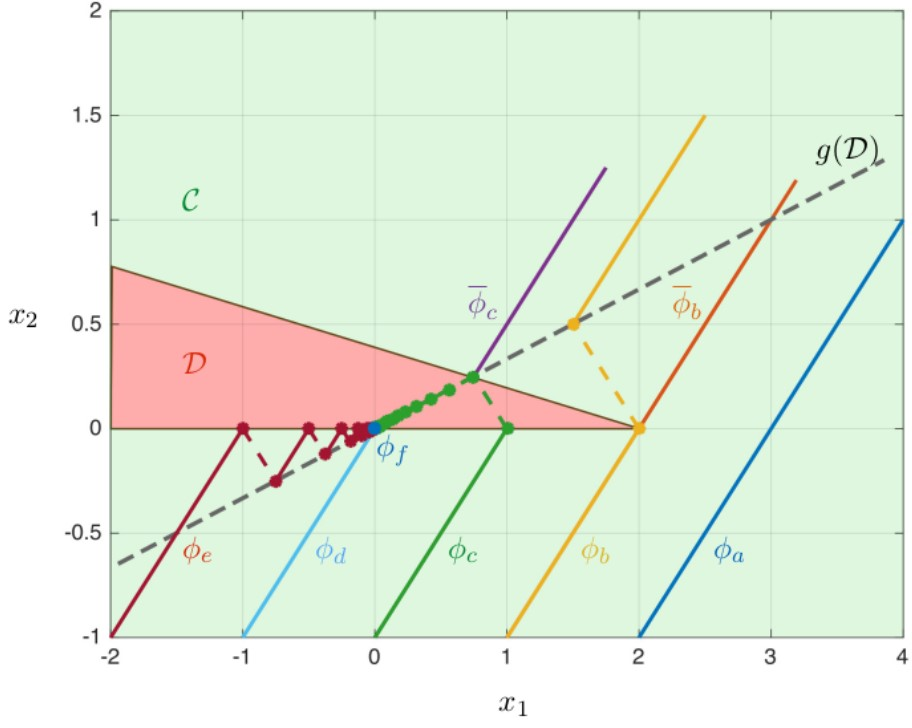
\includegraphics[width=10cm]{hybrid-example}
		\caption{graphical  representation of the solutions of $(\dagger)$.} \label{fig:hyb:example}
	\end{figure}
	Starting for example from an initial condition $\vet \phi(0,0)=(2,-1)$ we see that the system can only flow, thus solution $\vet \phi_a$ is drawn. Starting instead from $\vet \phi(0,0)=(1,-1)$ the solution flows up until the point $(2,0)$ where we have a \textit{bifurcation} of the solution (showing the non-uniqueness of the solution): we can either make a jump (solution $\vet \phi_b$) and then continue flowing or we can just flow (solution $\overline{\vet \phi}_b$).\\
	Starting from $\vet \phi(0,0) = (0,-1)$ we flow up to $(1,0)$ where we jump at $(3/4,1/4)$, a point that both in $\fset$ and $\jset$: we can so decide to flow or, more interestingly, entering a \textit{jump loop} where we converge to the point $(0,0)$ as shown in solution $\vet \phi_c$. \\
	Starting from $\vet \phi(0,0) = (-1,-1)$ we flow up to $(0,0)$ where we reach an \textit{equilibrium} as the jump doesn't allowed to further move away from that point (solution $\vet \phi_d$). One last example is starting by $\vet \phi(0,0) = (-2,-1)$ (solution $\vet \phi_e$) where the system with a \textit{loop} of flows and jumps converges to the point $(0,0)$.
	
	We call \de{complete solutions} the ones that are evolving forever; mathematically it means that the time $t+j\rightarrow \infty$.

\section{Stability of hybrid solutions}	
	We say that the \textbf{origin} of an hybrid system (H) is \de{Lyapunov stable} if for all $\varepsilon > 0$ there exists a $\delta > 0$ (function of $\varepsilon$) such that
	\[ |\vet \phi(0,0)| \leq \delta \quad \Rightarrow \quad |\vet \phi(t,j)|\leq \varepsilon \quad \forall (t,j) \in \textrm{dom}\{\vet \phi\} \]
	We say instead that the origin is \de{Lagrange stable} if for any $\delta > 0$ we can define a $\varepsilon > 0$ (function of $\delta$) such that
	\[ |\vet \phi(0,0)| \leq \delta \quad \Rightarrow \quad |\vet \phi(t,j)|\leq \varepsilon \quad \forall (t,j) \in \textrm{dom}\{\vet \phi\} \]
	As we can see the requirement for both Lyapunov and Lagrange stability is the same, but what changes is \textit{what we fix} and \textit{what we have to determine}: in the first case for any bound of the solution we search for a bound on the initial condition that makes the equality correct (and in general we can chose $\delta$ \textit{very small}), while the second statement implies a more stronger condition. Given in fact any offset from the origin we have to require that the solution \textit{doesn't diverge that much} (and stays bounded by a value $\varepsilon$).
	
	The origin is also said \de{globally attractive} \textbf{GA} if all solutions of the system are such that
	\[ \lim_{t+j\rightarrow \infty} |\vet \phi(t,j)| = 0 \]	
	If the origin is both Lyapunov stable and globally attractive, then it is also said \de{globally asymptotic stable} \textbf{GAS}.
	
	A solution is said \de{uniform globally stable} \textbf{UGS} if, for any initial condition, there exists an infinitely continuous function $\alpha \in C^\infty$ bounding the solutions, so for which
	\[ |\vet\phi(t,j) \leq \alpha\big(|\vet \phi(0,0)|\big) \qquad \forall (t,j)\in \textrm{dom}\{\vet \phi\} \]
	In practise this condition is met when the hybrid system is both Lyapunov and Lagrange stable.
	
	\paragraph{Hybrid system conditions} For the development of the Lyapunov theory, mostly of the time we will assume the \de{hybrid basic conditions} \textbf{HBC} of (H) requiring that
	\[ \tag{HbC} \fset,\jset \textrm{ are closed sets} \hspace{2cm} \vet f, \vet g \textrm{ are continuous functions} \]
	If this conditions are met, by proving that the system is GAS it will automatically tells us that is also \de{uniformly global asymptotic stable} \textbf{UGAS}.
	
\section{Lyapunov theory}
	The scope of the Lyapunov based theory for hybrid systems is to determine conditions that allow a system to be stable.
	
	\begin{theorem}
		The origin is globally asymptotic stable GAS (and if the hybrid basic conditions are met, then it's also UGAS) if and only if:
		\begin{itemize}
			\item it exists a continuously differentiable \de{Lyapunov function} $V:\x \mapsto V(\x) \in \mathds R$ such that 
			\[ \tag{S} \begin{cases}
				V(0) = 0 \\ V(\x) > 0 \quad & \forall \x \in \fset \cup \jset \setminus \{0\} \\
				\lim_{|\x|\rightarrow\infty} V(\x) = \infty & \x \in \fset \cup \jset
			\end{cases} \]
			implying so theta $V$ is positive definite and is radially bounded;
			\item it holds the \de{flow inequality}
			\[\tag{F'} \dot V(x) = \frac{\partial V}{\partial \x} \dx = \frac{\partial V}{\partial \x} \vet f(\x) < 0 \qquad \forall \x \in \fset\setminus\{0\} \]
			\item if holds the \de{jump inequality}
			\[ \tag{J'} \Delta V(\x) = V\big(\vet g(\x)\big) - V(\x) < 0 \qquad \forall \x \in \jset \setminus\{0\} \]
		\end{itemize}
	\end{theorem}
	The underlying idea behind this theory is that when the system is flowing (F), it's flowing to zero, while when it's jumping (J), it's jumping to zero. In practise the hardest thing to do is determine the Lyapunov function $V(\x)$ for the given hybrid system.
	
	Recalling the example of the bouncing ball, a candidate Lyapunov function is the one defines as
	\[ V(\x) = \frac 1 2 v^2 + \gamma p \]
	Observing that thus function is positive definite for all $\x \in \fset \cap \jset = \{ (p,v) \in \mathds R^2 \ : \ p\geq 0\}$, then we can compute
	\begin{align*}
		\dot V & = \frac 1 2 2 v\dot v + \rho \dot p = v(-\gamma) + \gamma v = 0 \\
		\Delta V & =\frac 1 2\big(v^+\big)^2 + \gamma p^+ - \frac 1 2 v^2 - \gamma p = \frac 1 2 (\lambda v)^2 - \frac 1 2 v^2 = - \frac 12 \big(1-\lambda^2\big) v^2
	\end{align*}
	As long as $\lambda < 1$ (physically, no energy is gained while bouncing but it's rather being lost), then we have that $\Delta V < 0$, proving that the system is uniformly globally asymptotic stable.
	
	
	
	
	
	
	
	
	
	
	
	
	
	
	
	
	
	
	
	
	
	
	
	
	
	
	\appendix
	
\end{document}